\documentclass[12pt,a4paper,openright,twoside]{book}
\usepackage[utf8]{inputenc}
\usepackage{disi-thesis}
\usepackage{code-lstlistings}
\usepackage{notes}
\usepackage{shortcuts}
\usepackage{acronym}
\usepackage{float}

\school{\unibo}
\programme{Corso di Laurea in Ingegneria e Scienze Informatiche}
\title{Layer geospaziali in Alchemist: acquisizione e interpolazione spazio-temporale di dati Copernicus}
\author{Emir Wanes Aouioua}
\date{\today}
\subject{Programmazione Ad Oggetti}
\supervisor{Prof. Gianluca Aguzzi}
\cosupervisor{Prof. Danilo Pianini}
\session{II}
\academicyear{2025-2026}

% Definition of acronyms
\acrodef{API}{Application Programming Interface}
\acrodef{IoT}{Internet of Thing}
\acrodef{JVM}{Java Virtual Machine}
% Copernicus
\acrodef{ECMWF}{European Centre for Medium-Range Weather Forecasts}
\acrodef{CEMS}{Copernicus Emergency Management Service}
\acrodef{CDS}{Climate Data Store}
\acrodef{EWDS}{Early Warning Data Store}
\acrodef{ADS}{Atmosphere Data Store}
\acrodef{EFAS}{European Flood Awareness System}
\acrodef{GloFAS}{Global Flood Awareness System}
\acrodef{CAMS}{Copernicus Atmosphere Monitoring Service}
\acrodef{C3S}{Copernicus Climate Change Service}
% OGC
\acrodef{OGC}{Open Geospatial Consortium}
% geofiles
\acrodef{GRIB}{GRIdded Binary}
\acrodef{NetCDF}{Network Common Data Form}
\acrodef{WMO}{World Meteorological Organization}
\acrodef{UCAR}{University Corporation for Atmospheric Research}
\acrodef{CF}{Climate and Forecast}
\acrodef{LAEA}{Lambert Azimuthal Equal Area}
% netcdf java
\acrodef{CDM}{Common Data Model}
\acrodef{XML}{Extensible Markup Language}

\mainlinespacing{1.241} % line spacing in mainmatter, comment to default (1)

\begin{document}

\frontmatter\frontispiece

\begin{abstract}	
Il simulatore Alchemist sa collocare i nodi di una simulazione su cartografia reale
e vincolarne il movimento alla rete stradale, ma le grandezze diffuse nell'ambiente
che può esporre loro sono prodotte solamente da regole fissate alla costruzione: nessuna
rappresenta misurazioni del mondo reale.

Questa tesi introduce un nuovo modulo che rende i dati distribuiti dal programma
Copernicus interrogabili dai nodi nel punto in cui si trovano e nell'istante
di simulazione in cui li richiedono. Il modulo riconduce file NetCDF e GRIB, il cui
schema non è fisso, a una rappresentazione uniforme di serie temporali di griglie
raster; produce un valore anche dove la posizione e l'istante richiesti non coincidono
con alcun campione, secondo regole di interpolazione e conversione intercambiabili,
scelte in funzione della semantica della grandezza da esporre; e acquisisce autonomamente
i dati dai data store Copernicus, conservandoli in una cache locale che consente il riuso
di questi ultimi senza nuove richieste di rete. Il risultato è additivo rispetto al
simulatore e configurabile in modo dichiarativo, senza scrivere codice.

La validazione comprende una suite di test indipendente dalla rete e una simulazione
dimostrativa costruita sugli eventi alluvionali che hanno colpito la Romagna nel
maggio 2023.
\end{abstract}

%\begin{dedication} % this is optional
%Optional. Max a few lines.
%\end{dedication}

%----------------------------------------------------------------------------------------
\tableofcontents   
\listoffigures     % (optional) comment if empty
\lstlistoflistings % (optional) comment if empty
%----------------------------------------------------------------------------------------

\mainmatter

%----------------------------------------------------------------------------------------
%\chapter{Introduzione}
%\label{chap:introduction}
%----------------------------------------------------------------------------------------

%\sidenote{Add sidenotes in this way. They are named after the author of the thesis}
%that you are discussing \acp{vm},
%ou may need both \ac{vm} and \acp{vm}.
%\note{At the end, describe the structure of the paper}

%\paragraph{Structure of the Thesis}

%----------------------------------------------------------------------------------------
% CAPITOLO 1 (INTRODUZIONE)
%----------------------------------------------------------------------------------------

\chapter{Introduzione}
\label{cap:introduzione}

\section{Contesto e motivazioni}
\label{sec:contesto-e-motivazioni}

La simulazione è uno degli strumenti utilizzati per studiare sistemi formati
da molte entità che interagiscono fra loro e con lo spazio in cui si trovano:
reti di dispositivi, flotte di veicoli, gruppi di persone che si spostano in
un'area urbana. Quando lo scenario di riferimento è collocato in un luogo reale,
l'attendibilità di un esperimento non dipende solamente dal comportamento
dei suoi attori, ma anche da quanto fedelmente è riprodotto l'ambiente in
cui essi agiscono.

Di quell'ambiente fanno parte grandezze che variano da un punto all'altro e
lungo il tempo, e che non vengono prodotte dagli attori: la portata di un fiume,
la temperatura dell'aria, la concentrazione di inquinanti in atmosfera, il pericolo
d'incendio di una zona boschiva. Chi si trova sul territorio non può controllarle,
le percepisce, e vi reagisce prendendo decisioni: cambiando percorso, diramando un
allarme, coordinandosi con altri attori. Queste misure costituiscono
lo stimolo esterno rispetto al quale il comportamento degli attori di una
simulazione prende significato.

Grandezze di questo genere, per buona parte del pianeta, sono misurate,
ricostruite e pubblicate con continuità. Copernicus\footnote{Il programma Copernicus: \url{https://www.copernicus.eu/it}.},
il programma di osservazione della Terra dell'Unione Europea, distribuisce liberamente archivi
che coprono decenni di storia, i quali spaziano dalle rianalisi climatiche ai
sistemi di allerta alluvionale. Eventi realmente accaduti dispongono quindi
di descrizioni quantitative pubbliche, consultabili rispetto a istanti temporali
e posizioni diverse.

Che quei dati siano pubblici e accessibili non basta però perché un attore,
nel corso di una simulazione, possa chiedere quanto valga una grandezza
nel punto in cui si trova. I dati sono pubblicati in formati binari specialistici,
organizzati secondo convenzioni della comunità scientifica che li produce,
e vanno richiesti a servizi remoti che li preparano su richiesta, impiegando
un tempo variabile e senza garanzia di riuscita. Soprattutto, sono campionati,
quindi noti solamente in corrispondenza dei punti di una griglia e di una
successione di istanti temporali, mentre la posizione di un attore, e il
momento in cui esso interroga l'ambiente, sono quantità continue che un
simulatore misura a partire dall'inizio della simulazione.

Alchemist~\cite{alchemist}, il simulatore di sistemi complessi sviluppato
presso l'Università di Bologna su cui si aggiunge questo lavoro, possiede già
la maggior parte di ciò che serve per collocare un esperimento in un luogo preciso:
sa caricare cartografia reale, disporvi gli attori e vincolarne il movimento
alla rete stradale. Ciò che non possiede è un modo per far percepire loro una
misurazione campionata in una posizione geografica. Le grandezze diffuse
nell'ambiente sono rappresentate da un'astrazione dedicata, il \emph{layer}, le cui
realizzazioni disponibili producono però valori calcolati da regole fissate
al momento della costruzione. Una simulazione può quindi essere accurata nel
collocare i propri nodi ma non altrettanto in ciò che essi percepiscono una
volta collocati. 

\section{Il contributo di questa tesi}
\label{sec:contributo}

Il lavoro qui descritto colma questa distanza con un nuovo modulo del
simulatore, che rende i dati distribuiti da Copernicus interrogabili dagli
attori come grandezza diffusa nell'ambiente, nel punto in cui l'attore
si trova e nell'istante di simulazione in cui lo chiede.

Per fare in modo che ciò sia possibile occorre leggere file il cui schema non
è noto a priori e ricondurli a una rappresentazione uniforme; produrre un valore
anche dove una misura non è disponibile, secondo un criterio che non può essere
unico perché dipende da che cosa la grandezza rappresenta; e ottenere i dati
dai servizi Copernicus senza alcun intervento manuale, conservandoli in locale
in modo che esecuzioni successive non debbano richiederli una seconda volta.
Il tutto senza modificare le astrazioni del modello del simulatore, e in modo
dichiarabile direttamente nel file di configurazione di una simulazione,
senza scrivere codice.

Il codice sorgente del modulo, nella versione documentata in questa tesi, è
archiviato in modo permanente e liberamente
consultabile\footnote{Archivio permanente del modulo: \url{https://archive.softwareheritage.org/swh:1:dir:1246f419d7f827ab6a7767d13f922af4845632c9;origin=https://github.com/Wanes01/Alchemist;visit=swh:1:snp:1145cad987574aa5003aa00de817ba00591905e3;anchor=swh:1:rev:58f72d98e0b10428b192d8e555a357f0da7366c6;path=/alchemist-geospatial/}}.

\section{Struttura della tesi}
\label{sec:struttura-della-tesi}

La tesi è strutturata nei seguenti capitoli:

\begin{itemize}
  \item \textbf{Contesto} (\Cref{chap:contesto}): vengono descritti gli elementi su cui il
  lavoro poggia: le parti del simulatore inerenti al progetto, i servizi attraverso
  cui Copernicus distribuisce i propri dati, i formati e le convenzioni con cui
  questi sono codificati e lo standard a cui si ispirano le richieste remote.

  \item \textbf{Analisi} (\Cref{chap:analisi}): si scompone il problema nelle sue parti e
  se ne ricavano i requisiti che la soluzione deve soddisfare, vengono discusse le questioni che
  vanno delimitate prima di poter essere tradotte in scelte progettuali e si individuano le
  entità in gioco.

  \item \textbf{Progettazione} (\Cref{chap:progettazione}): viene esposta la struttura che
  deriva dall'analisi, ovvero la suddivisione del modulo, le astrazioni che compongono
  ciascuna delle sue parti e le decisioni che le attraversano.

  \item \textbf{Implementazione} (\Cref{chap:implementazione}): ci si sofferma sui punti
  in cui la realizzazione ha richiesto scelte non deducibili dalla progettazione, imposte
  dal formato dei dati, dal comportamento dei servizi remoti o dal meccanismo con
  cui Alchemist istanzia i componenti di una simulazione.

  \item \textbf{Validazione} (\Cref{chap:validazione}): vengono riportate le evidenze
  del corretto funzionamento del modulo, le quali comprendono la suite di test
  automatici, le verifiche condotte al di fuori di essi e una simulazione dimostrativa
  che impiega l'intera catena su dati reali, costruita attorno agli eventi alluvionali
  che hanno colpito la Romagna nel maggio 2023.

  \item \textbf{Conclusioni} (\Cref{chap:conclusioni}): viene tracciato un bilancio
  del lavoro rispetto agli obiettivi, vengono dichiarati i limiti del lavoro e
  si indicano le direzioni di sviluppo che la struttura realizzata rende possibili. 
\end{itemize}


%----------------------------------------------------------------------------------------
% CAPITOLO 2 (CONTESTO)
%----------------------------------------------------------------------------------------

\chapter{Contesto}
\label{chap:contesto}

\section{Il simulatore Alchemist}
\label{sec:alchemist}

Alchemist~\cite{alchemist} è un simulatore di sistemi complessi, scritto in Java e
Kotlin, nato alla fine del 2010 come sottoprodotto del progetto europeo SAPERE e
mantenuto da allora come progetto open source da Danilo Pianini e collaboratori presso
il Dipartimento di Informatica dell'Università di Bologna.

In Alchemist una simulazione è composta da un \emph{environment}, lo spazio in cui
vivono i \emph{nodi}. Ciascun nodo è un contenitore di \emph{molecole} (identificatori,
l'equivalente di un nome di variabile) a cui sono associate \emph{concentrazioni},
i valori che esse assumono, e di \emph{reazioni}, gli eventi che ne modificano lo stato
nel tempo. Il metamodello è mostrato nella \Cref{fig:metamodel}.

\begin{figure}[H]
    \centering
    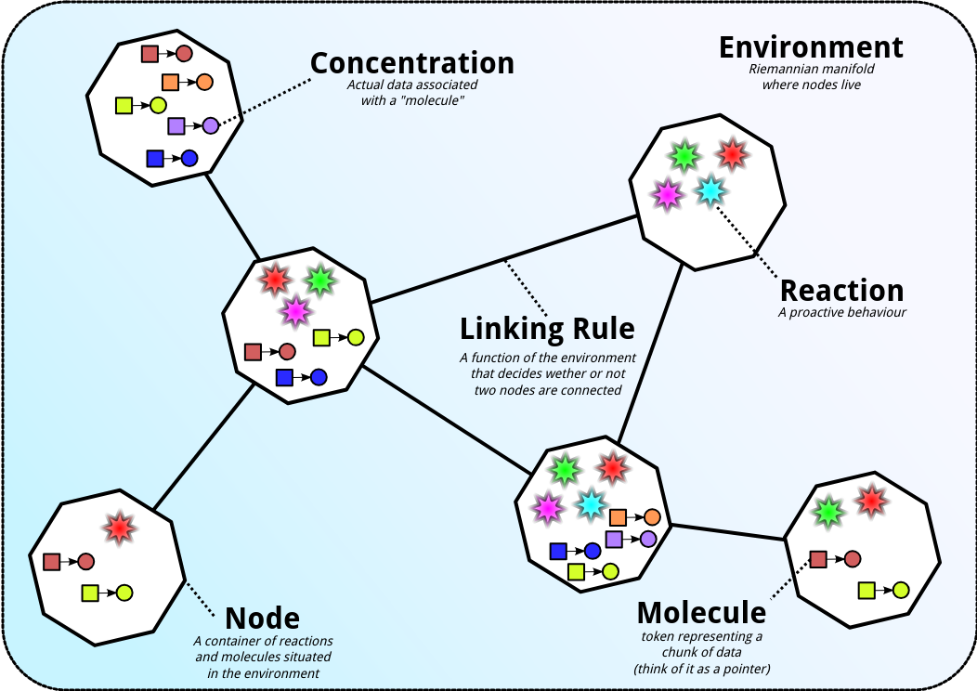
\includegraphics[width=\linewidth]{figures/alchemist/metamodel.png}
    \caption[Il metamodello di Alchemist]{Il metamodello di Alchemist. Immagine tratta dal sito ufficiale del simulatore~\protect\footnotemark.}
    \label{fig:metamodel}
\end{figure}
\footnotetext{Spiegazione del metamodello di Alchemist: \url{https://alchemistsimulator.github.io/explanation/metamodel/}.}

Alchemist è impiegato come strumento in diversi lavori di ricerca.
Ad esempio, in~\cite{aguzzi2022dynamic} è stato usato per simulare, sull'area urbana di Toronto,
un sistema \ac{IoT} decentralizzato di allerta alluvionale: i valori di pioggia
misurati da una rete di pluviometri, ricavata da dati reali, vengono aggregati
in modo distribuito per pre-allertare le stazioni dei vigili del fuoco prossime alle
zone a rischio. In~\cite{audrito2021optimal} il simulatore costituisce invece l'intero
apparato sperimentale del lavoro: viene utilizzato sia per confrontare algoritmi
decentralizzati di raccolta e aggregazione dei dati su reti di dispositivi mobili,
esplorando parametri quali densità, diametro della rete e velocità
di movimento, sia per uno studio in cui gli stessi algoritmi vengono applicati
al tracciamento di una folla in un parco cittadino.

Le sezioni che seguono si limitano agli elementi necessari a collocare il lavoro
descritto in questa tesi: la nozione di layer, il modo in cui il tempo di simulazione è
reso accessibile ai componenti, il supporto geospaziale già disponibile e il sistema di
caricamento delle simulazioni da file YAML.

\subsection{Il motore di simulazione}
\label{subsec:alchemist-lifecycle}

Una simulazione Alchemist nasce da una configurazione dichiarativa
(Sezione~\ref{subsec:alchemist-loader}), a partire dalla quale sono istanziati
l'environment, i layer, i nodi con le rispettive reazioni e contenuti. Il modello
che ne risulta descrive lo stato iniziale della simulazione.

A metterlo in esecuzione è il motore, un simulatore a eventi discreti la cui implementazione si
fonda sul \emph{Next Reaction Method} di Gibson e Bruck~\cite{gibson}. Il motore
procede per passi: a ogni passo viene selezionata, fra tutte le reazioni
schedulate, quella il cui istante di esecuzione è il più vicino; il tempo di simulazione
assume tale istante; la reazione viene eseguita, modificando lo stato del modello;
infine vengono rischedulate le reazioni la cui esecuzione dipende da quella appena
avvenuta. Il tempo non avanza quindi a passi costanti, ma per salti da un evento al
successivo, e fra due eventi consecutivi lo stato del modello resta invariato.

Il punto d'ingresso del motore è la \texttt{Simulation}, che custodisce il tempo di simulazione
corrente ed espone i comandi per avviare, sospendere e arrestare l'esecuzione. Lo stato
in cui essa si trova è descritto da un insieme predefinito di valori, dall'inizializzazione
alla terminazione, ed è interrogabile in qualunque momento.

\subsection{Il concetto di \emph{layer}}
\label{subsec:alchemist-layer}

Le molecole e le concentrazioni descrivono lo stato interno dei singoli nodi. Alcune
grandezze, però, non appartengono ad alcun nodo in particolare: sono proprietà
dell'ambiente stesso, definite in ogni suo punto indipendentemente dal fatto che vi si
trovi o meno un nodo a percepirle. La temperatura, l'intensità luminosa, la
concentrazione di un inquinante in atmosfera sono esempi di questo tipo: un nodo che
si muove nello spazio ne osserva valori diversi non perché il proprio stato sia
cambiato, ma perché è cambiata la sua posizione.

Alchemist modella queste grandezze attraverso il concetto di \emph{layer}: una
sovrapposizione di dati distribuita sull'ambiente, associata a una molecola e
interrogabile da qualunque punto dello spazio. Formalmente, un \texttt{Layer<T, P>} è
una funzione che associa a ogni posizione di tipo \texttt{P} dell'environment un
valore di tipo \texttt{T}. L'interfaccia si riduce a un solo metodo:

\lstinputlisting[language=Java,label={lst:layer-interface}]{listings/Layer.java}

Un nodo può quindi interrogare un
layer con la propria posizione corrente e ottenere il valore che il layer associa a
quel punto, usandolo per esempio come stimolo a cui reagire.

Le implementazioni preesistenti in Alchemist realizzano però tutte layer
che producono valori sintetici, determinati da una regola fissata alla costruzione, come
\sloppypar{\texttt{BidimensionalGaussianLayer}}, che descrive una distribuzione
gaussiana bidimensionale centrata su un punto. Queste realizzazioni sono adeguate a
rappresentare fenomeni il cui comportamento varia rispetto a una formula,
ma non un fenomeno misurato: i dati ambientali reali non sono
espressi da una funzione, bensì campionati su griglie spaziali a risoluzione
finita, disponibili solo in corrispondenza di determinati istanti e distribuiti in
formati binari specialistici.

\subsection{Il tempo di simulazione}
\label{subsec:alchemist-time}

Alchemist rappresenta l'istante corrente di una simulazione come un valore scalare di tipo
\texttt{Time}, privo di un'unità di misura intrinseca: la sua interpretazione è una convenzione
lasciata al modellista della simulazione (ad esempio secondi, ore, giorni), non
un vincolo imposto dal simulatore; il suo tempo parte da zero e cresce con l'avanzare degli eventi.

Il tempo di simulazione appartiene al motore, che viene creato solo quando il modello è
già completo. Un componente, nel momento in cui viene costruito, non ha quindi ancora
alcun tempo da leggere: può ottenerlo soltanto durante l'esecuzione, interrogando la
\texttt{Simulation} attraverso l'environment.

Un layer, in particolare, riceve come unico argomento la posizione da cui è interrogato
(Sezione~\ref{subsec:alchemist-layer}): se il valore che restituisce dipende anche dal
tempo, è il layer stesso a doverselo procurare per questa via.

\subsection{Il supporto geospaziale preesistente}
\label{subsec:alchemist-osm}

Alchemist offre un supporto già maturo per simulazioni su cartografia
reale: un \texttt{OSMEnvironment} può caricare estratti di OpenStreetMap e collocare i
nodi al suo interno, vincolandone il movimento a una rete stradale e delegando il calcolo
dei percorsi a GraphHopper~\footnote{Motore di calcolo dei percorsi GraphHopper: \url{https://www.graphhopper.com/}.}.
Le posizioni in questi ambienti sono espresse come \texttt{GeoPosition}, coppie di
latitudine e longitudine. È questa asimmetria che fa nascere il problema affrontato in questa tesi:
un simulatore capace di collocare e muovere con precisione i propri nodi nello spazio geografico reale, ma
non dotato di un modo per far percepire loro misurazioni campionate nello spazio.

\subsection{Il caricamento delle simulazioni da YAML}
\label{subsec:alchemist-loader}

Una simulazione Alchemist si specifica tipicamente in modo dichiarativo, in un file YAML
che indica, per ciascun componente, il nome della classe che lo implementa e i parametri
con cui costruirlo. Questo meccanismo, basato sulla reflection, non è un semplice dettaglio
di configurazione: i vincoli che impone hanno condizionato la forma di ogni classe destinata
a essere istanziata da YAML.

Il layer gaussiano introdotto nella Sezione~\ref{subsec:alchemist-layer} è costruito dal
seguente costruttore, di sei parametri, di cui il primo (\texttt{baseline}) e l'ultimo
(\texttt{sigmaY}) sono opzionali:

\lstinputlisting[language=Kotlin,label={lst:bidimensional-gaussian-layer-kotlin}]{listings/BidimensionalGaussianLayer.kt}

Il loader individua la classe indicata dalla chiave \texttt{type}, ne seleziona un
costruttore compatibile con gli argomenti forniti e lo invoca tramite reflection. Nella
forma più diretta, i parametri sono specificati posizionalmente:

\lstinputlisting[language=YAML,label={lst:bidimensional-gaussian-layer}]{listings/bidimensional.yml}

la chiave \texttt{molecule} indica la molecola a cui il layer viene associato
nell'environment, mentre \texttt{parameters} elenca gli argomenti del costruttore. I
quattro valori forniti vengono associati, nell'ordine, a \texttt{centerX},
\texttt{centerY}, \texttt{norm} e \texttt{sigmaX}, mentre \texttt{baseline} e
\texttt{sigmaY} assumono i rispettivi valori di default. La costruzione equivalente, se
scritta direttamente in Kotlin, sarebbe:

\lstinputlisting[language=Kotlin,label={lst:bidimensional-gaussian-equivalent}]{listings/bidimensional-equivalent.kt}

Che i parametri opzionali possano essere omessi non è però una capacità del loader: gli
argomenti di default sono una nozione di Kotlin, invisibile alla reflection della \ac{JVM}, e a
renderli accessibili è l'annotazione \texttt{@JvmOverloads} presente nel
costruttore, la quale istruisce il compilatore a generare costruttori aggiuntivi, ottenuti
rimuovendo i parametri dotati di default a partire dall'ultimo. Ne
discende che da YAML si può omettere soltanto un
suffisso della lista dei parametri opzionali. Per specificare \texttt{sigmaY} occorrerebbe
fornire anche \texttt{baseline}, che lo precede.
L'ordine in cui i parametri opzionali sono dichiarati non è quindi indifferente.

Oltre che per via posizionale, i parametri possono essere specificati anche tramite il
nome dell'argomento a cui si riferiscono:

\lstinputlisting[language=YAML,label={lst:bidimensional-gaussian-layer-named}]{listings/bidimensional-names.yml}

Questa forma elimina l'ambiguità sull'ordine e rende esplicito a quale parametro ciascun
valore si riferisca, ma resta soggetta al vincolo appena descritto.

Non tutti i parametri, infine, provengono dal file YAML: le entità già costruite al momento
dell'istanziazione, fra cui l'environment stesso, sono iniettate automaticamente laddove un
parametro ne dichiari il tipo, e non compaiono quindi fra quelli dichiarati nella
configurazione.

L'istanza risultante viene registrata, nell'environment, in corrispondenza della molecola
indicata dalla chiave \texttt{molecule} (\texttt{moleculeName}).

\section{Il programma Copernicus e i suoi servizi di dati}
\label{sec:copernicus}

Copernicus~\footnote{Il programma Copernicus: \url{https://www.copernicus.eu/it}.}
è il programma di osservazione della Terra dell'Unione Europea, articolato in
servizi tematici. Fra questi, il \ac{CEMS} %\footnote{\url{https://emergency.copernicus.eu/}}
fornisce informazioni geospaziali a supporto della gestione di emergenze ed eventi di
protezione civile, ed è il servizio da cui ha preso avvio il progetto descritto in questa
tesi.

L'accesso programmatico ai dati non è però organizzato per servizio: avviene attraverso
una famiglia di \emph{data store} gestiti dall'\ac{ECMWF}~\footnote{Centro Europeo per le previsioni meteorologiche a medio termine: \url{https://www.ecmwf.int/}}
e costruiti sulla stessa
infrastruttura software, differenziati per host e per il dominio dei dataset che
espongono:

\begin{itemize}
    \item il \ac{CDS}, data store del \ac{C3S}, che ospita fra gli altri ERA5, la
    rianalisi climatica globale prodotta da \ac{ECMWF};
    \item l'\ac{EWDS}, data store del \ac{CEMS}, che ospita i dataset di \ac{EFAS} e
    \ac{GloFAS}, sistemi di allerta alluvionale rispettivamente a scala europea e
    globale, e quelli relativi agli incendi boschivi;
    \item l'\ac{ADS}, data store del \ac{CAMS}, relativo a composizione atmosferica,
    qualità dell'aria, gas serra e radiazione solare.
\end{itemize}

I tre condividono la stessa infrastruttura, per cui un unico
client è sufficiente a interrogarli tutti, e la differenza si riduce all'host e al
catalogo dei dataset disponibili.

L'autenticazione verso i tre data store avviene tramite un unico token \ac{ECMWF}:
la stessa identità è valida su \ac{CDS}, \ac{EWDS} e \ac{ADS}, e viene letta da un file di configurazione
locale nel formato \texttt{.cdsapirc}~\footnote{Struttura del file \texttt{.cdsapirc}: \url{https://cds.climate.copernicus.eu/how-to-api}},
lo stesso adottato dal client Python ufficiale di \ac{ECMWF}.

\section{Formati e convenzioni per dati raster geospaziali}
\label{sec:formati-raster}

I dataset offerti dai tre data store descritti precedentemente sono forniti,
a seconda del dataset e della selezione effettuata in fase di richiesta, in due
formati binari pensati per la memorizzazione di dati geospaziali multidimensionali
campionati su una griglia: \ac{GRIB} e \ac{NetCDF}. Entrambi distribuiscono i valori
di una o più grandezze fisiche su assi di latitudine, longitudine e tempo, dove l'asse temporale
è una successione di istanti assoluti associati a un calendario di riferimento. Nel
dettaglio:

\begin{itemize}
\item \ac{GRIB}, distribuito dai data store nelle versioni GRIB1 e GRIB2, è uno standard
    binario definito dalla \ac{WMO}, con l'obiettivo di
    trasmettere in modo efficiente i grandi volumi di dati prodotti dai modelli
    meteorologici. Un file \ac{GRIB} non è autosufficiente dal punto di vista semantico:
    la grandezza fisica contenuta è identificata da codici numerici, il cui significato è
    definito da tabelle esterne, standard o specifiche del centro meteorologico di
    origine. Ad esempio, nella tabella 128 di \ac{ECMWF} il codice 167 identifica la
    temperatura registrata a due metri dal suolo~\footnote{Tabella ECMWF per i file GRIB che esprimono la temperatura a due metri dal suolo: \url{https://codes.ecmwf.int/grib/param-db/167}},
    ma la corrispondenza fra codice e
    grandezza fisica non è ricavabile dal solo contenuto del file;
\item \ac{NetCDF}, distribuito dai data store nelle versioni NetCDF3 e NetCDF4, è un formato
    sviluppato e mantenuto da Unidata, un programma comunitario dell'\ac{UCAR},
    orientato all'accesso e alla condivisione di dati scientifici
    multidimensionali. A differenza di \ac{GRIB}, un file \ac{NetCDF} è
    autodescrittivo: nomi delle variabili, unità di misura e altri metadati
    sono incorporati nel file stesso. Il formato di per sé impone però una
    struttura minima; per questo la comunità scientifica ha definito
    convenzioni che ne regolano il contenuto: nome e ordine delle dimensioni,
    attributi obbligatori, semantica degli assi. La più diffusa, e adottata
    dagli store di riferimento, è la convenzione \ac{CF}~\cite{cf_conventions}, \Cref{fig:netcdf-structure}.
\end{itemize}

\begin{figure}[H]
    \centering
    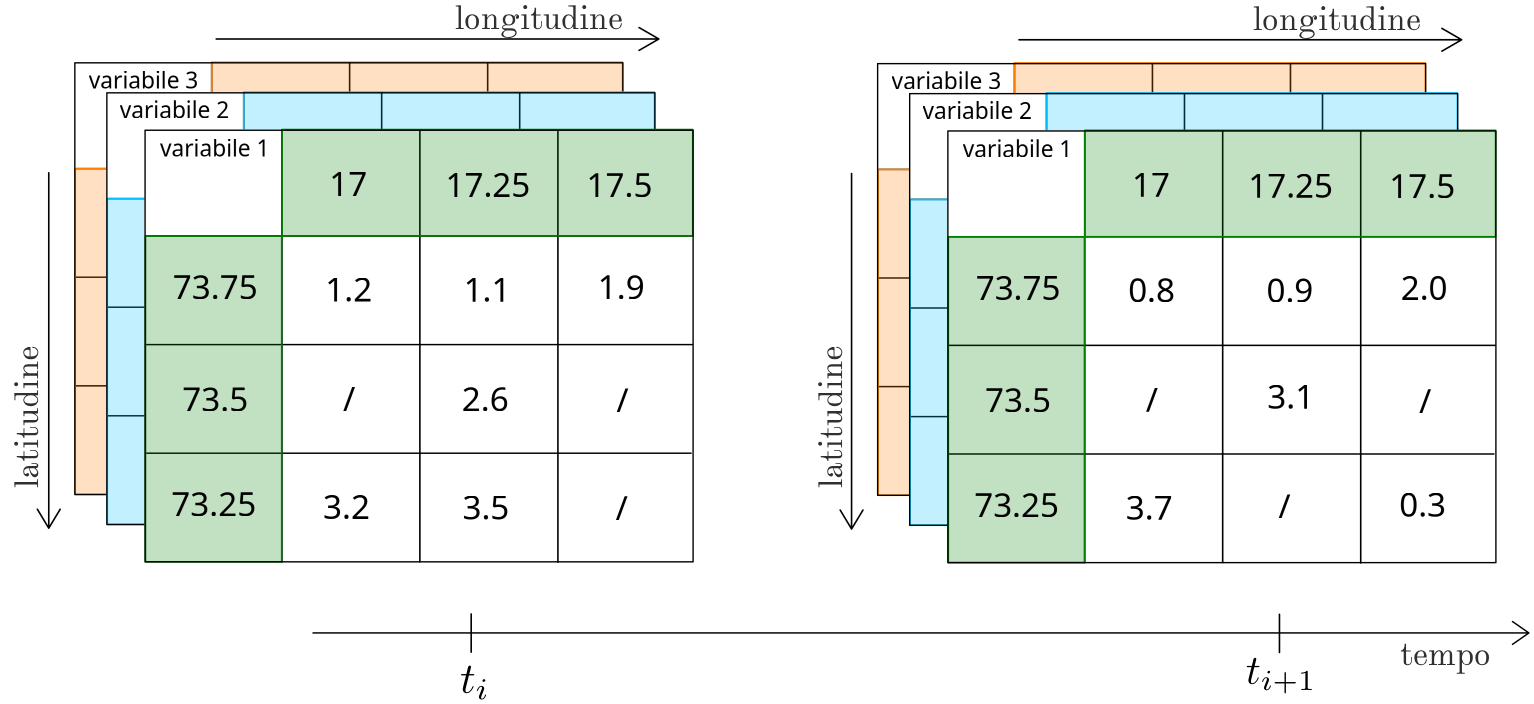
\includegraphics[width=0.75\linewidth]{figures/netcdf-file-structure.png}
    \caption[Struttura CF di un file NetCDF]{Struttura CF di un file NetCDF. Immagine tratta da \cite{simulating_complexity_netcdf}.}
    \label{fig:netcdf-structure}
\end{figure}

Un aspetto comune ai due formati riguarda la rappresentazione dei valori mancanti, che nei
dataset forniti dai data store non è un caso raro: le misure di portata fluviale, ad esempio,
sono definite solo in corrispondenza dei corsi d'acqua, e lasciano prive di valore tutte
le altre celle della griglia. 
%In un file \ac{NetCDF} conforme alle convenzioni \ac{CF}
%l'assenza di un valore è segnalata dall'attributo \texttt{\_FillValue} o \texttt{missing\_value}:
%un valore riservato, che le librerie di lettura riconoscono come indicatore di dato mancante.~\cref{fig:netcdf-structure}

%In un file \ac{GRIB} lo stesso ruolo è svolto da una sezione dedicata,
%la \emph{bitmap section}, che indica punto per punto della griglia se il valore
%corrispondente sia presente. Il modo in cui queste due rappresentazioni vengono
%ricondotte a un'unica convenzione interna è
%discusso nel Capitolo~\ref{chap:implementazione}.

Un secondo aspetto, comune a entrambi i formati, riguarda la nozione di
\emph{griglia raster}. Nella sua forma più diffusa, una griglia raster è
definita dal prodotto cartesiano di un asse di latitudini e uno di longitudini,
indipendenti fra loro: ogni cella è quindi individuabile con una coppia di
coordinate geografiche. Questa non è però l'unica struttura possibile.
Alcuni dei dataset distribuiti dai data store sono definiti su una griglia nativa espressa in
una proiezione cartografica, ad esempio \ac{LAEA}, non riconducibile al prodotto
cartesiano di due assi indipendenti di latitudine e longitudine.

Un punto rilevante, con conseguenze dirette sulle scelte implementative,
riguarda la spaziatura degli assi. La convenzione \ac{CF} richiede che
latitudine e longitudine siano strettamente monotone, ma non equispaziate, e
sull'asse temporale il vincolo non è più forte: un dataset può
contenere misurazioni a intervalli di tempo non regolari.
Nel caso di \ac{GRIB} la questione non si pone nemmeno in
termini di convenzione, dal momento che un file è una successione di
griglie indipendenti, ciascuna con il proprio istante di validità: nulla
nel formato impone che l'insieme risultante sia ordinato, né tanto meno
regolare.

\section{Il paradigma OGC API Processes}
\label{sec:ogc-api-processes}

Le richieste di dati verso i tre data store Copernicus sono operazioni di durata variabile,
da qualche secondo a diverse decine di minuti in base all'entità della richiesta, e vengono
quindi gestite in modo asincrono: il client sottomette una richiesta, ottiene l'indirizzo a
cui interrogarne lo stato, e lo interpella periodicamente fino al completamento
dell'elaborazione.

Lo schema è descritto, a livello di standard, da \ac{OGC} in \emph{OGC API - Processes -
Part 1: Core}~\cite{ogc_api_processes_core}, che specifica un'interfaccia REST per
l'esecuzione di elaborazioni remote e per il recupero dei relativi risultati. Il ciclo di
vita di un job si articola in tre fasi:
la sottomissione, tramite una richiesta \texttt{POST} all'endpoint di esecuzione del
processo; l'interrogazione dello stato, il cui indirizzo lo standard prescrive sia
comunicato al client nell'intestazione \texttt{Location} della risposta alla
sottomissione; e il recupero dei risultati, disponibile una volta che il job ha raggiunto
uno stato terminale. Lo standard definisce inoltre l'insieme degli stati che un job può
assumere durante l'elaborazione, distinguendo quelli intermedi da quelli terminali, ai
quali è associata la disponibilità dei risultati o della descrizione dell'errore.

Ogni risposta include, oltre ai dati che rappresenta, un vettore \texttt{links}. Ciascun
collegamento è accompagnato da una relazione (\texttt{rel}), un'etichetta che ne dichiara
il significato: quale risorsa il collegamento raggiunga e in che rapporto stia con quella
corrente. Lo standard stabilisce quali relazioni usare per le risorse che definisce, ad
esempio \texttt{status} per lo stato di un job, e consente alle implementazioni di
aggiungere collegamenti propri, oltre a quelli previsti.

Per gli errori, lo standard raccomanda, senza imporlo, il formato \emph{Problem Details}
definito dalla RFC 7807~\cite{rfc7807}, che uniforma la struttura del corpo delle risposte
di errore e la rende interpretabile.

I data store \ac{ECMWF} si ispirano a questo paradigma, ma se ne discostano su più punti,
alcuni dei quali non documentati. Tali scostamenti hanno determinato scelte
implementative del sottosistema di acquisizione, e sono discussi nel Capitolo ~\ref{chap:implementazione}.
\emph{\textbf{("??" = link al capitolo di implementazione, attualmente assente)}}

%----------------------------------------------------------------------------------------
% CAPITOLO 3 (ANALISI)
%----------------------------------------------------------------------------------------

\chapter{Analisi}
\label{chap:analisi}

\section{Analisi del problema}
\label{sec:analisi-problema}

Come anticipato nella Sezione~\ref{subsec:alchemist-osm}, il supporto geospaziale di
Alchemist consente di collocare e muovere con precisione i nodi di una simulazione su
cartografia reale, ma non offre un modo altrettanto maturo per esporre loro dati geospaziali,
in un dato istante, nel punto dello spazio geografico in cui si trovano.
L'interfaccia \texttt{Layer<T, P>} (Sezione~\ref{subsec:alchemist-layer}) è generica sia
nella posizione \texttt{P} sia nel valore \texttt{T} restituito, ma nessuna delle sue
implementazioni preesistenti espone dati che rappresentino misurazioni del mondo reale.

I dati geospaziali misurati, quali quelli distribuiti dai data store Copernicus descritti
nella Sezione~\ref{sec:copernicus}, differiscono dai valori sintetici prodotti dalle
implementazioni preesistenti per diversi aspetti:

\begin{itemize}
    \item sono distribuiti in un formato specialistico (\ac{NetCDF} o \ac{GRIB},
    Sezione~\ref{sec:formati-raster}), il cui schema (quali dimensioni compaiano, in quale
    ordine, con quale direzione degli assi, con quale nome interno la grandezza di interesse
    sia identificata) non è fissato a priori, ma varia da dataset a dataset;
    \item sono campionati su una griglia sia nello spazio sia nel tempo, mentre la
    posizione richiesta a un layer e l'istante di simulazione corrente sono entrambi
    quantità continue: fra un campione e l'altro non esiste, nel dato
    originale, alcun valore, e va quindi stabilita una regola per produrne uno;
    \item ciascuna griglia è riferita a un istante assoluto del mondo reale, espresso
    secondo un calendario, mentre il tempo di una simulazione Alchemist è un valore scalare
    privo di unità di misura intrinseca (Sezione~\ref{subsec:alchemist-time}), la cui
    interpretazione è una convenzione lasciata al modellista;
    \item non tutte le celle di una griglia riportano una misura: i formati prevedono un
    valore convenzionale per quelle che ne sono prive;
    \item non sono calcolabili localmente, vanno ottenuti da un
    servizio remoto che risponde in modo asincrono, secondo il paradigma descritto nella
    Sezione~\ref{sec:ogc-api-processes}, senza garanzia di completamento della richiesta.
\end{itemize}

Questi aspetti individuano i seguenti sotto-problemi:

\begin{enumerate}
    \item \textbf{Rappresentazione}: come rappresentare in memoria, in modo indipendente dalla fonte
    specifica del dato, una serie temporale di griglie raster geospaziali, le cui celle possono
    non ospitare una misurazione;
    \item \textbf{Risoluzione}: date una posizione geografica e un istante di simulazione
    arbitrari, come stabilire a quale istante del mondo reale essi corrispondano e come
    produrre un valore a partire da campioni discreti nello spazio e nel tempo, con
    possibili misurazioni mancanti;
    \item \textbf{Acquisizione}: come ottenere questi campioni da un servizio remoto asincrono, in modo
    riproducibile e verificabile, senza doverli riscaricare a ogni esecuzione della
    simulazione.
\end{enumerate}

\iffalse
I tre sotto-problemi sono debolmente accoppiati fra loro: la rappresentazione di una serie
di griglie è indipendente dalla loro provenienza, la risoluzione di un valore lo è dal modo
in cui le griglie sono state ottenute, e l'acquisizione lo è dal modo in cui i dati
acquisiti verranno successivamente letti. L'unico punto di contatto è la forma in cui i
dati vengono consegnati, ovvero un insieme di file in uno dei formati descritti nella
Sezione~\ref{sec:formati-raster}.
\fi

\section{Obiettivi}
\label{sec:obiettivi}

L'obiettivo generale del lavoro è dotare Alchemist della capacità di esporre ai nodi
di una simulazione grandezze geospaziali misurate, in funzione della posizione che essi
occupano e dell'istante di simulazione in cui vi accedono, ottenendole dai data store
Copernicus.

Per ogni sotto-problema individuato nella sezione precedente viene individuato
un sotto-obiettivo:

\begin{enumerate}
    \item \textbf{Rappresentazione}: definire una rappresentazione in memoria di una serie
    temporale di griglie raster geospaziali che sia indipendente dal formato e dalla fonte
    da cui i dati provengono, e che tenga conto sia dell'estensione spaziale e temporale
    entro la quale la grandezza è nota, sia dell'assenza di misura in alcune delle sue
    celle;

    \item \textbf{Risoluzione}: rendere tale rappresentazione interrogabile in una posizione
    geografica e a un istante di simulazione arbitrari. Ciò comprende lo stabilire quale
    istante del mondo reale corrisponda a un dato tempo di simulazione, e quale valore
    restituire quando la posizione e l'istante così individuati non coincidono con alcun
    campione disponibile; la regola con cui tale valore viene prodotto deve poter essere
    scelta in funzione della semantica della grandezza esposta, anziché essere fissata una
    volta per tutte;

    \item \textbf{Acquisizione}: dotare il simulatore della capacità di ottenere
    autonomamente dai data store Copernicus i dati necessari a una simulazione,
    conservandoli localmente in modo che esecuzioni successive che utilizzano gli stessi
    dati possano riutilizzarli.
\end{enumerate}

\iffalse
A questi si affianca un quesito preliminare. La proposta iniziale del lavoro ipotizzava che
l'interfaccia dei layer di Alchemist (Sezione~\ref{subsec:alchemist-layer}) dovesse essere
rivista per accogliere dati provenienti da fonti esterne. Stabilire se e in che misura ciò
sia necessario è parte dell'analisi, e ne condiziona il perimetro: la
Sezione~\ref{subsec:api-sufficiente} vi risponde una volta delimitati i requisiti.
\fi

Il risultato atteso è quindi un nuovo modulo del simulatore che aggiunga quanto descritto,
i cui componenti siano dichiarabili direttamente nella configurazione di una simulazione.

\section{Requisiti}
\label{sec:requisiti}

\subsection{Requisiti funzionali}
\label{subsec:requisiti-funzionali}

\begin{itemize}
    \item \textbf{F1 (Interrogazione spaziale)}: \label{req:F1} il modulo deve restituire
    un valore per una posizione geografica arbitraria interna all'estensione spaziale
    coperta dai dati.

    \item \textbf{F2 (Interrogazione temporale)}: \label{req:F2} il valore restituito deve
    essere quello percepito rispetto all'istante di simulazione corrente.

    \item \textbf{F3 (Corrispondenza temporale)}: \label{req:F3} la relazione fra il tempo
    di simulazione e gli istanti del mondo reale a cui i dati sono riferiti deve essere
    dichiarabile da chi conduce la simulazione, e non fissata dal modulo.

    \item \textbf{F4 (Risoluzione fra campioni)}: \label{req:F4} il modulo deve produrre un
    valore anche quando la posizione richiesta e l'istante individuato non coincidono con
    alcuno dei campioni disponibili.

    \item \textbf{F5 (Intercambiabilità della regola)}: \label{req:F5} la regola con cui
    tale valore viene prodotto deve poter essere scelta fra più alternative, senza
    richiedere modifiche al modulo.

    \item \textbf{F6 (Tipo esposto configurabile)}: \label{req:F6} il tipo del valore
    esposto ai nodi non deve coincidere necessariamente con quello numerico con cui la
    grandezza è registrata nel file, così da poter rappresentare anche grandezze la cui
    interpretazione non è puramente quantitativa.

    \item \textbf{F7 (Valori mancanti espliciti)}: \label{req:F7} le celle prive di misura
    presenti nei dati originali devono essere trattate in modo esplicito, e non ignorate o
    sostituite silenziosamente.

    \item \textbf{F8 (Indipendenza dal dataset)}: \label{req:F8} il modulo deve operare, con
    lo stesso codice, su più dataset e più data store Copernicus
    (Sezione~\ref{sec:copernicus}), senza conoscerne a priori lo schema.

    \item \textbf{F9 (Acquisizione autonoma)}: \label{req:F9} il modulo deve ottenere
    autonomamente i dati non ancora disponibili localmente e conservarli in una cache la
    cui posizione sia configurabile.

    \item \textbf{F10 (Riuso dei dati acquisiti)}: \label{req:F10} i dati già presenti in
    cache devono essere riutilizzati quando la configurazione della richiesta è invariata,
    senza effettuare nuove richieste di rete.

    \item \textbf{F11 (Configurazione dichiarativa)}: \label{req:F11} il modulo deve essere
    configurabile da un file YAML di simulazione (Sezione~\ref{subsec:alchemist-loader})
    senza richiedere obbligatoriamente la scrittura di codice; ciò vale anche per la scelta
    fra le alternative previste da \req{F5}.
\end{itemize}

\subsection{Requisiti non funzionali}
\label{subsec:requisiti-non-funzionali}

\begin{itemize}
    \item \textbf{NF1 (Additività)}: \label{req:NF1} il modulo deve realizzarsi come
    estensione del simulatore, senza richiedere modifiche al suo motore né alle astrazioni
    del suo modello.

    \item \textbf{NF2 (Genericità)}: \label{req:NF2} la parte che sa leggere e risolvere una
    serie temporale di griglie raster deve restare separata da quella che sa ottenerle dai
    data store Copernicus, così che la prima resti utilizzabile anche con fonti diverse da
    quelle qui considerate.

    \item \textbf{NF3 (Aderenza alle convenzioni di Alchemist)}: \label{req:NF3} il codice è
    destinato a una pull request verso il repository del simulatore, e deve quindi
    rispettarne le convenzioni di stile, di collocazione dei package e di configurazione
    degli strumenti di analisi statica.

    \item \textbf{NF4 (Testabilità senza rete)}: \label{req:NF4} nessun test deve dipendere
    dalla disponibilità dei data store Copernicus o dal possesso di credenziali valide.

    \item \textbf{NF5 (Riproducibilità)}: \label{req:NF5} la stessa richiesta verso un data
    store deve corrispondere in modo deterministico alla stessa voce di cache.

    \item \textbf{NF6 (Fallimento esplicito)}: \label{req:NF6} nessuna condizione anomala
    deve produrre un valore silenziosamente scorretto: deve produrre un errore con un
    messaggio diagnostico.

    \item \textbf{NF7 (Fallimento anticipato)}: \label{req:NF7} le condizioni che
    impediscono a una simulazione di disporre dei dati di cui ha bisogno devono
    manifestarsi al caricamento della simulazione, e non durante l'esecuzione.

    \item \textbf{NF8 (Costo dell'interrogazione)}: \label{req:NF8} il valore di un layer
    viene richiesto potenzialmente molte volte per ogni evento della simulazione: la lettura
    non deve comportare accessi a risorse esterne, e il suo costo non deve dipendere dalla
    provenienza dei dati.

    \item \textbf{NF9 (Uso concorrente della cache)}: \label{req:NF9} Alchemist consente
    l'esecuzione simultanea di più simulazioni; più esecuzioni che condividano la stessa
    cache e richiedano gli stessi dati non devono interferire fra loro, né produrre voci di
    cache incomplete o corrotte.
\end{itemize}

\section{Analisi dei requisiti}
\label{sec:analisi-requisiti}

Alcuni dei requisiti elencati richiedono un ragionamento preliminare, o pongono condizioni
la cui portata va delimitata prima di poter essere tradotte in scelte progettuali.

\subsection{La corrispondenza fra i domini temporali}
\label{subsec:corrispondenza-temporale}

Il requisito \req{F3} chiede di mettere in relazione due domini temporali di natura
diversa: gli istanti assoluti del mondo reale a cui i dati sono riferiti e il tempo
scalare della simulazione. La relazione può essere stabilita in due modi opposti:
eliminando la differenza alla radice, ovvero sostituendo il tipo di tempo del simulatore
con uno che rappresenti già un istante assoluto, oppure mantenendo il tipo esistente e
stabilendo una corrispondenza esplicita, confinandola nel componente che ne ha bisogno.

La prima strada è stata oggetto di uno studio di fattibilità, condotto sul codice del
simulatore con l'obiettivo di stimare l'estensione dell'intervento piuttosto che di
portarlo a termine.

L'ostacolo principale è di natura semantica. \texttt{Time} è oggi usato
indifferentemente per denotare un istante della simulazione e un intervallo fra due
istanti distinti: le due nozioni condividono lo stesso tipo e sono combinabili fra loro
tramite operazioni aritmetiche. Le astrazioni di \texttt{kotlin.time} le distinguono
invece in due tipi separati, \texttt{Instant} e \texttt{Duration}, fra i quali solo alcune
combinazioni sono ammesse: ad esempio, non è possibile moltiplicare un istante per uno
scalare. Allo stesso modo non si ha consistenza nel tipo di ritorno delle operazioni,
ad esempio sottrarre un \texttt{Instant} da un altro produce un \texttt{Duration}, mentre
\texttt{Time} ammette tutte queste operazioni e il loro risultato è sempre del medesimo
tipo. La sostituzione non è quindi meccanica: richiede di stabilire, per ogni punto d'uso,
quale dei due ruoli vi sia svolto, e la modifica di una firma si propaga a tutti i suoi
utilizzatori.

Un intervento di questa natura ricade sul motore del simulatore e sulle astrazioni del suo
modello, ed è quindi incompatibile con \req{NF1}. Si è pertanto scelto di percorrere la
seconda strada: mantenere inalterato il tipo di tempo del simulatore e stabilire la
corrispondenza fra i due domini nel solo componente che ne ha bisogno, dichiarata da chi
configura la simulazione come \req{F3} richiede.

\subsection{La discretezza dei campioni}
\label{subsec:discretezza-campioni}

Risolta la corrispondenza temporale, resta il problema posto da \req{F4}: quale valore
restituire quando l'istante richiesto cade fra due istanti campionati; formalmente, quale
valore restituire quando a ogni istante $t_{i}$ è associata una griglia spaziale e si ha
che il tempo di simulazione corrente $t_s \in [t_i, t_{i+1}]$, \Cref{fig:temp-interp}.

\begin{figure}[H]
    \centering
    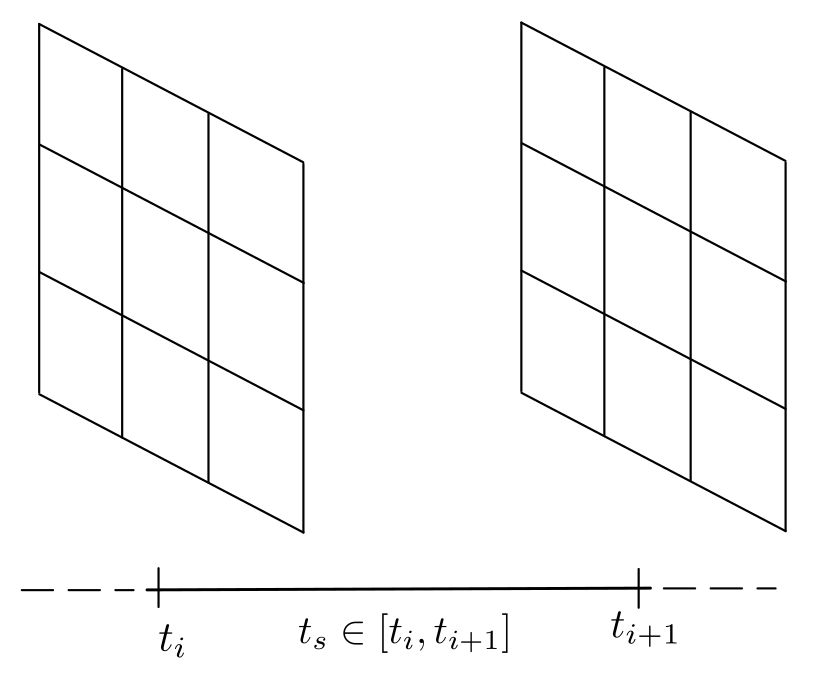
\includegraphics[width=0.6\linewidth]{figures/temporal_interpolation.png}
    \caption[Composizione temporale dei campioni]{L'istante identificato ricade nell'intervallo di due campionamenti.}
    \label{fig:temp-interp}
\end{figure}

E in modo del tutto analogo,
quando la posizione richiesta cade fra le celle della griglia spaziale; formalmente,
quale valore restituire per la posizione $P = (\text{lat}_{a}, \text{lon}_{b})$ quando
$\text{lat}_{a} \in [\text{lat}_{i}, \text{lat}_{i+1}]$ e $\text{lon}_{b} \in [\text{lon}_{j}, \text{lon}_{j+1}]$
, \Cref{fig:spatial-interp}.

\begin{figure}[H]
    \centering
    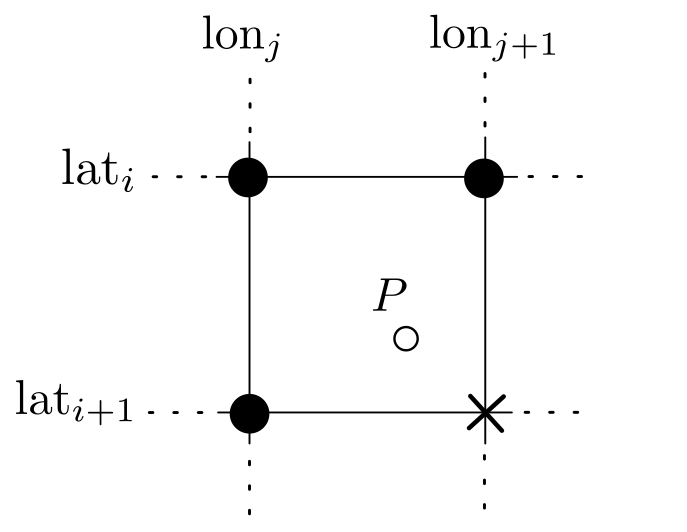
\includegraphics[width=0.5\linewidth]{figures/spatial_interpolation.png}
    \caption[Composizione spaziale dei campioni]{La posizione richiesta ricade tra le misurazioni. I cerchi pieni rappresentano misurazioni disponibili,
    la croce rappresenta una misurazione assente.}
    \label{fig:spatial-interp}
\end{figure}

La risposta richiede una regola di combinazione dei campioni adiacenti, e tale regola non
può essere unica. Una grandezza che varia con continuità, come la temperatura, ammette
naturalmente una combinazione pesata dei campioni che la circondano; al contrario, un dato
di natura categorica (come il codice convenzionale che distingue pioggia, neve o grandine)
non ammette interpolazioni intermedie: tali grandezze richiedono di selezionare un singolo
campione secondo un criterio esplicito, ad esempio il campione spazialmente più vicino.
La scelta dipende dalla semantica del dato, non dal meccanismo che lo espone, e non può
quindi essere fissata una volta per tutte nel codice del modulo.

È questa osservazione a motivare \req{F5}: la regola con cui un valore viene prodotto a
partire dai campioni disponibili, sia temporali sia spaziali, deve essere configurabile e
intercambiabile.

La stessa regola è inoltre il punto in cui si decide come comportarsi con le celle prive di
misura, di cui \req{F7} chiede un trattamento esplicito: se una posizione richiesta è
circondata anche da un solo campione assente, non esiste una risposta valida per ogni
grandezza, e la decisione se propagare l'assenza, ignorarla o convertirla ricade nuovamente
sulla semantica del dato.

\subsection{Il dominio di definizione del layer}
\label{subsec:estensione-spaziale}

I requisiti \req{F1} e \req{F2} sono formulati su una posizione geografica e un istante di
simulazione arbitrari: va stabilito entro quali confini tale arbitrarietà sia ammissibile.

Sul dominio spaziale, ogni dataset copre una regione geografica delimitata, e una posizione
esterna a essa non corrisponde ad alcuna misura. Produrre comunque un valore, ad esempio
riportando la posizione al bordo della copertura, significherebbe restituire un numero
plausibile ma privo di fondamento nei dati, tanto più fuorviante quanto più la posizione
richiesta è lontana dalla regione coperta; ciò contrasterebbe con \req{NF6}, che vieta la
produzione di valori silenziosamente scorretti. Il layer è quindi definito sulla sola
estensione spaziale dei dati che espone, e una richiesta al di fuori di essa è da
considerarsi un errore di modellazione della simulazione, da segnalare come tale.

La delimitazione è sostenibile perché l'estensione spaziale è nota prima
dell'esecuzione: essa coincide con l'area richiesta al data store, e la collocazione
dei nodi e i percorsi lungo i quali essi si muovono ricadono su chi configura
la simulazione. Una posizione esterna è quindi data da un'incoerenza fra i
dati richiesti e l'ambiente simulato.

\iffalse
Sul dominio temporale la situazione è diversa. Il tempo di simulazione può avanzare
indefinitamente a partire dallo zero. Rifiutare la richiesta, come sul dominio
spaziale, significherebbe interrompere una simulazione altrimenti valida. Il layer resta
quindi definito sull'intero asse temporale, e la regola con cui produce un valore al di
fuori dell'intervallo coperto è discussa nel Capitolo~\ref{chap:progettazione}.
\fi

Sul dominio temporale la situazione è diversa. Il tempo di una simulazione avanza
indefinitamente a partire dallo zero, e il momento in cui essa termina non è
necessariamente noto a chi la configura. Alchemist consente di dichiarare condizioni
di terminazione, verificate dopo ogni evento, ma non ne richiede per forza una.

Ne consegue che una limitazione sul dominio temporale avrebbe una portata diversa da
quello sul dominio spaziale. Sul dominio spaziale il rifiuto segnala un'incoerenza
fra i dati richiesti e l'ambiente simulato, per la quale nessuna risposta sarebbe
corretta. Sul dominio temporale interromperebbe invece una simulazione potenzialmente
coerente.

Il layer resta quindi definito sull'intero asse temporale, e la regola con cui
produce un valore al di fuori dell'intervallo coperto è discussa nella
Sezione~\ref{sec:corrispondenza-temporale}.

\subsection{Le ipotesi sui dati utilizzati}
\label{subsec:griglie-supportate}

Il requisito \req{F8} chiede che il modulo operi, con lo stesso codice, su dataset diversi
senza conoscerne a priori lo schema. Perché ciò sia possibile occorre stabilire che cosa
tali dataset debbano avere in comune, ovvero quali proprietà siano date per acquisite
sui dati di ingresso.

Due discendono direttamente da ciò che il layer espone. La prima è che la grandezza di
interesse dipenda dalle sole tre dimensioni tempo, latitudine e longitudine: sono le sole
rispetto alle quali il layer viene interrogato (\req{F1}, \req{F2}), e un dataset definito
anche su altre dimensioni, come la quota o il livello di pressione, non individuerebbe un
valore unico per una posizione e un istante. La seconda è che i file che descrivano una
stessa serie condividano la medesima griglia e la medesima grandezza, ovvero l'omogeneità
che la Sezione~\ref{sec:modello-dominio} attribuisce a una serie di griglie.

La terza è invece una restrizione effettiva del campo di applicabilità: si assume che la
griglia spaziale sia definita da un asse di latitudini e uno di longitudini indipendenti e
strettamente monotoni, non necessariamente a passo costante. Come osservato nella
Sezione~\ref{sec:formati-raster}, non tutti i dataset distribuiti dai data store la
soddisfano: alcuni sono campionati su una griglia nativa in una proiezione cartografica,
nella quale le coordinate geografiche di ciascuna cella sono note ma non ottenibili come
prodotto cartesiano di due assi indipendenti. Individuare la cella che contiene una data
posizione richiede allora di invertire la proiezione fra il sistema di riferimento del
dataset e quello geografico.

La restrizione è stata ritenuta accettabile perché la forma di distribuzione
prevalente prevede una griglia in latitudine e longitudine, sulla quale il
servizio consente di ritagliare l'area geografica di interesse al momento della richiesta.

Sul dominio temporale non viene invece posta alcuna ipotesi oltre alla distinzione e
all'ordinamento degli istanti: l'ampiezza degli intervalli che li separano può variare
liberamente lungo la serie.

\subsection{Il momento del fallimento}
\label{subsec:momento-del-fallimento}

L'acquisizione dei dati da un servizio remoto, richiesta da \req{F9}, è l'unica parte del
lavoro soggetta a condizioni fuori dal controllo del modulo: la rete può non essere
disponibile, le credenziali possono mancare o essere scadute, il servizio può rifiutare la
richiesta o consegnare dati incompleti.

Il requisito \req{NF7} stabilisce che tutte queste condizioni si manifestino al momento del
caricamento della simulazione: una simulazione parte solo se dispone di tutti i dati di
cui ha bisogno, altrimenti non parte affatto, segnalando il motivo.

La scelta garantisce una proprietà utile a chi conduce esperimenti: il fallimento è
immediato e riconoscibile, anziché manifestarsi a esecuzione avanzata sotto forma di
risultati alterati.

\subsection{L'adeguatezza dell'interfaccia dei layer}
\label{subsec:api-sufficiente}

La revisione dell'interfaccia dei layer era fra le ipotesi di partenza
del progetto: \texttt{Layer<T,P>} è stata concepita per grandezze calcolabili
localmente, ed è lecito chiedersi se sia adeguata ad accogliere dati misurati
provenienti da fonti esterne. Delimitati i requisiti, la domanda viene affrontata
verificando quali fra essi pongano condizioni sulla forma dell'interrogazione
anziché sul modo in cui il valore viene prodotto.

Nessuno fra i requisiti funzionali riguarda la forma con cui il valore viene richiesto:
tutti riguardano il modo in cui esso viene prodotto. In particolare, \req{F1}, \req{F2} e \req{F4} pongono
condizioni sul valore restituito da un'interrogazione la cui firma resta quella esistente;
\req{F3} riguarda una corrispondenza fissata alla costruzione del layer;
\req{F5}, \req{F6} e \req{F7} riguardano componenti interni al layer; \req{F8}, \req{F9} e
\req{F10} riguardano l'origine dei dati, che il layer riceve già costruiti; \req{F11}
riguarda il meccanismo di caricamento, esterno all'interfaccia.

Resta una sola limitazione, ed è di natura diversa. Il valore restituito da un layer che
espone dati misurati può, in linea di principio, cambiare in due modi distinti: perché il
tempo di simulazione avanza e il layer legge un istante diverso di una serie di dati già
disponibile, oppure perché il dato sottostante viene aggiornato dall'esterno durante
l'esecuzione. Il primo caso è quello descritto da \req{F2}, e non pone alcun problema
all'interfaccia esistente: la lettura resta funzione della sola posizione richiesta e del
tempo di simulazione corrente. Il secondo richiederebbe invece un layer mutabile durante
l'esecuzione, il quale è a sua volta subordinato a una revisione del motore reattivo di
Alchemist non ancora disponibile.

\iffalse
Di conseguenza la serie di dati esposta dal layer è fissata al momento della costruzione
e non muta per l'intera durata della simulazione. Con questa delimitazione, e una volta
separate la lettura dei dati, la regola di combinazione dei campioni e la loro
acquisizione, l'interfaccia esistente si è rivelata adeguata così com'è.

Ne consegue che \req{NF1} è soddisfacibile: il lavoro qui descritto è puramente additivo
rispetto al simulatore, e si realizza come un nuovo modulo che implementa un'interfaccia
esistente, senza richiedere modifiche al motore né alle astrazioni del suo modello.
\fi

Con questa delimitazione, e una volta separate la lettura dei dati, la regola
di combinazione dei campioni e la loro acquisizione, l'interfaccia esistente si è
rivelata adeguata così com'è. Di conseguenza \req{NF1} è rispettabile: il lavoro qui descritto
è puramente additivo rispetto al simulatore, e si realizza come un nuovo modulo che implementa
un'interfaccia esistente.

\section{Modello del dominio}
\label{sec:modello-dominio}

Questa sezione individua le entità in gioco e le relazioni che le legano; la
\Cref{fig:modello-dominio} le riporta. Il modello si limita alle astrazioni: le loro
realizzazioni concrete e il modo in cui vengono composte fra loro sono presentate nel
Capitolo~\ref{chap:progettazione}. Per ciascuna entità sono indicati i requisiti a cui
essa risponde.

\begin{figure}[H]
    \centering
    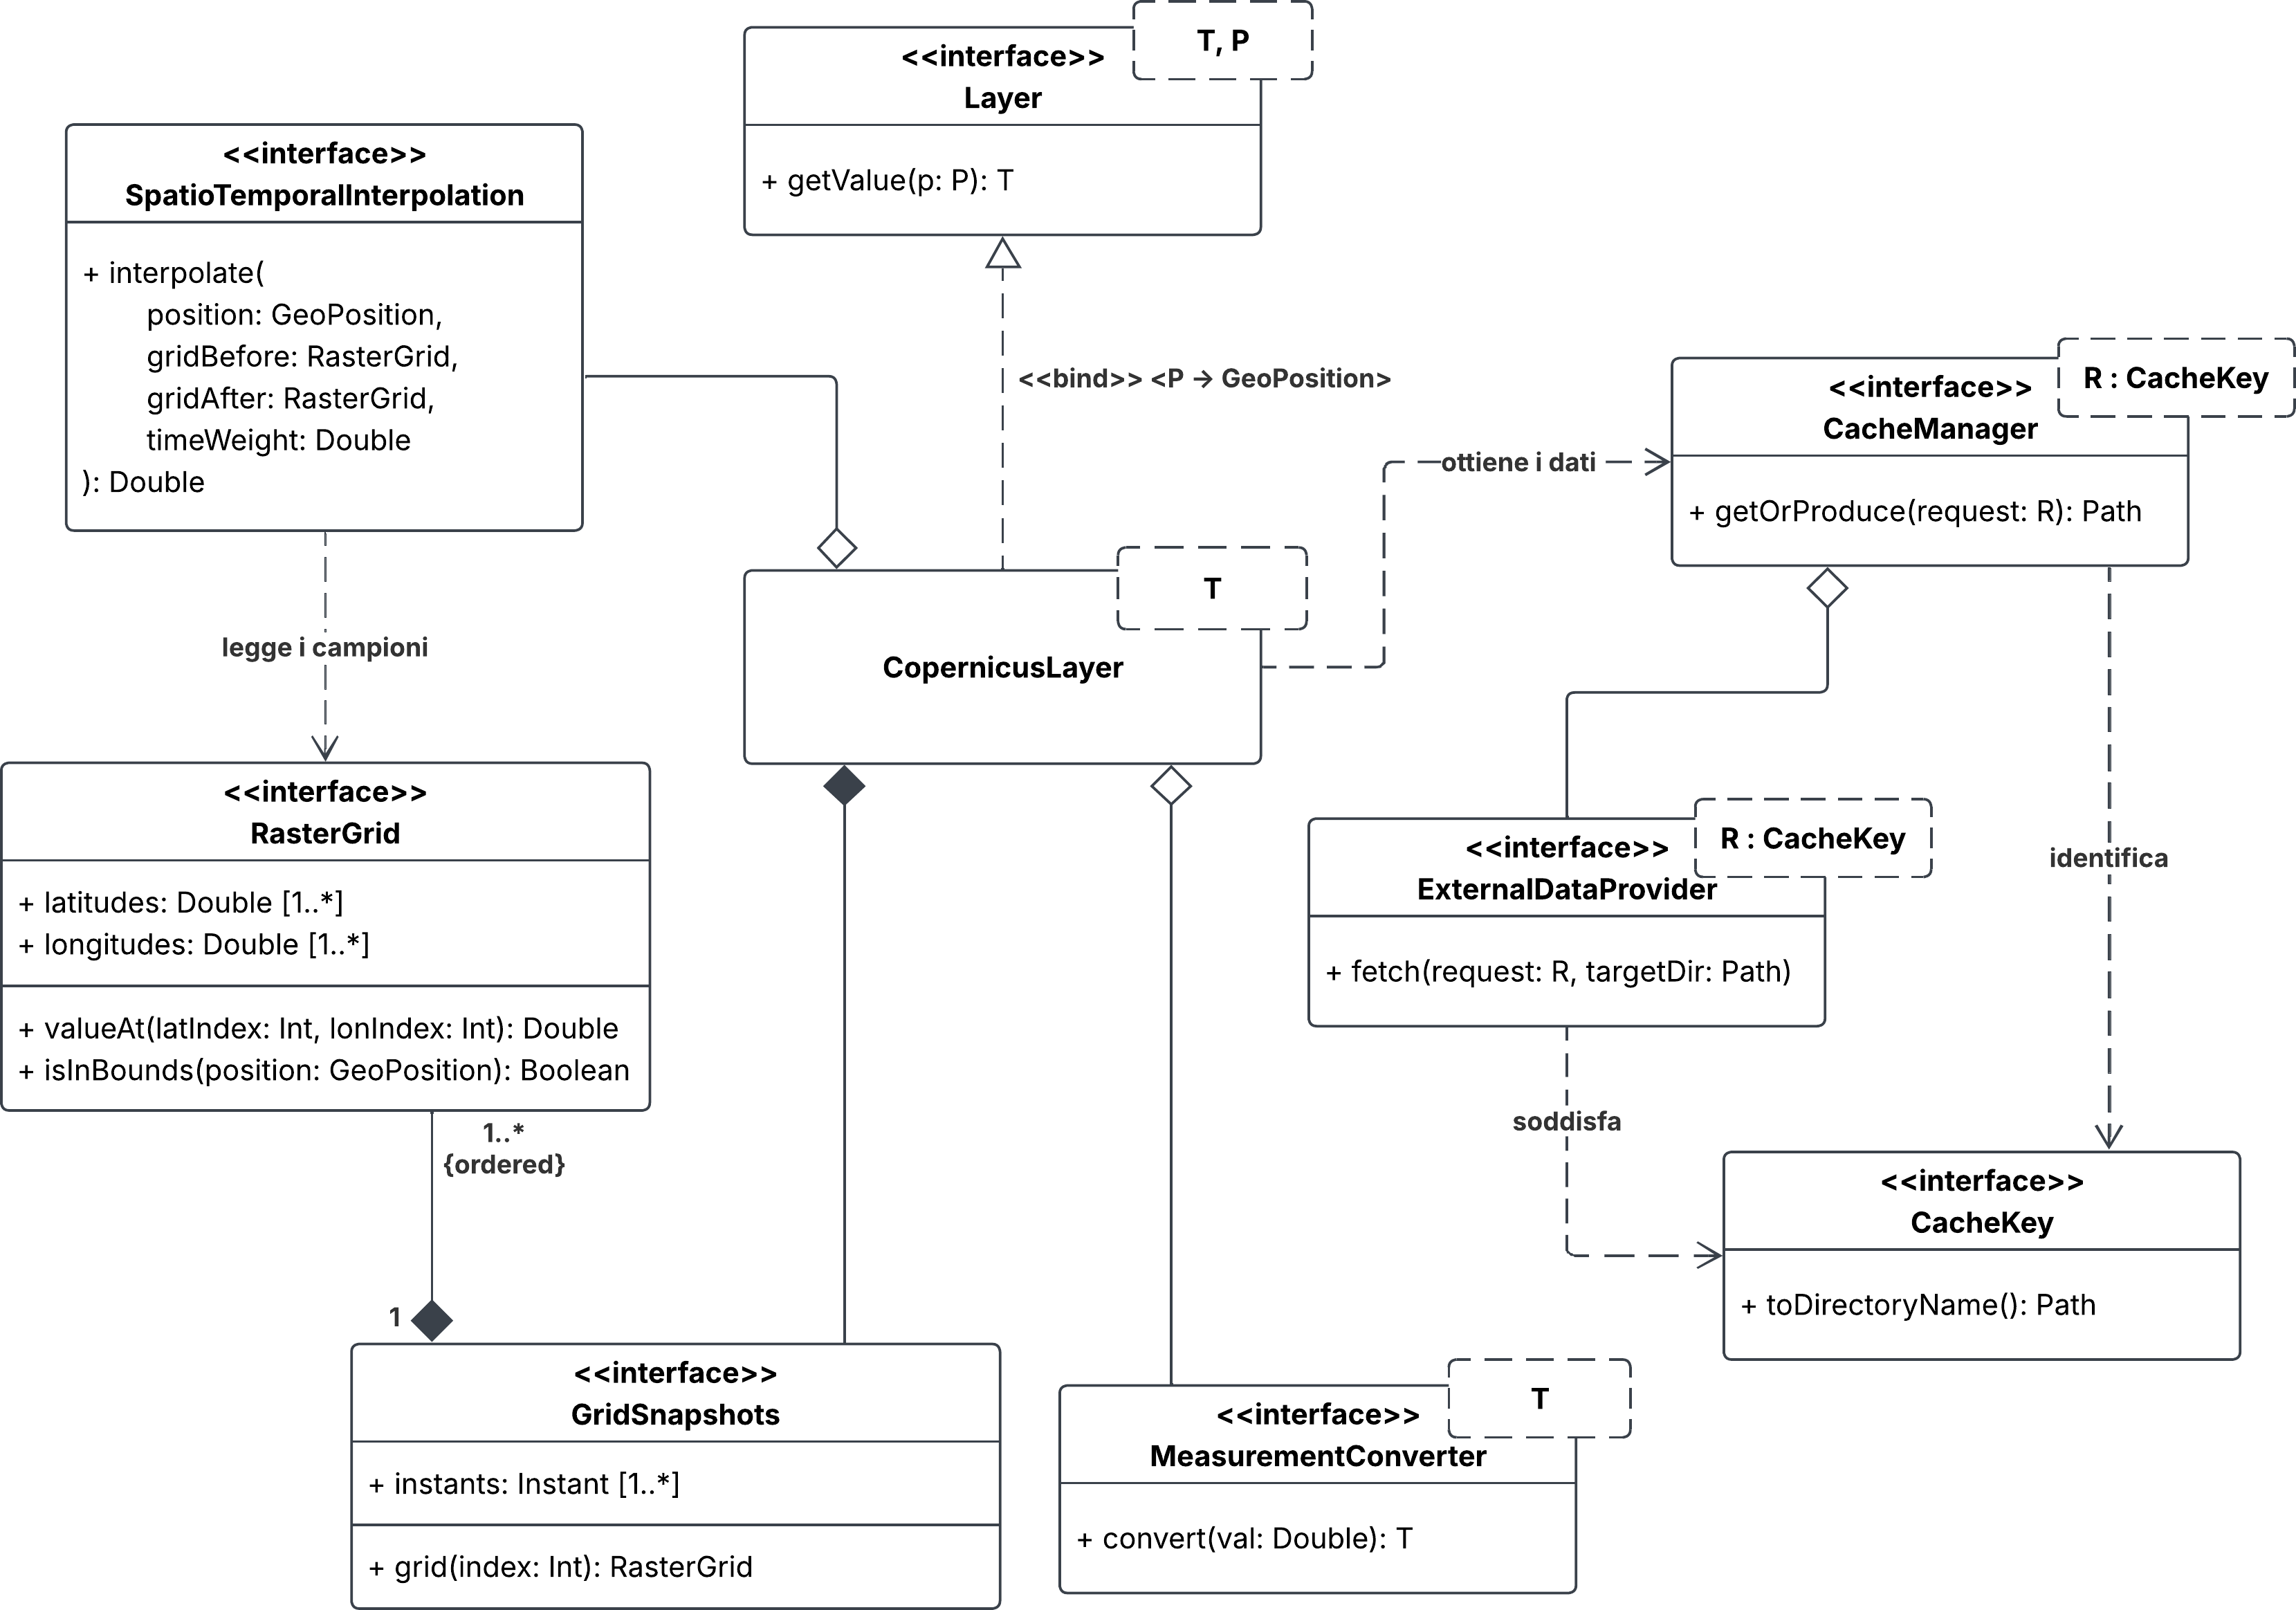
\includegraphics[width=\linewidth]{figures/uml_dominio.png}
    \caption[Modello del dominio]{Le entità del dominio e le relazioni fra di esse.}
    \label{fig:modello-dominio}
\end{figure}

\begin{itemize}
    \item \texttt{RasterGrid} (\req{F1}, \req{F7}, \req{F8}): l'insieme dei campioni di una
    grandezza relativi a un singolo istante, organizzati su un reticolo definito da un asse
    di latitudini e uno di longitudini indipendenti e strettamente monotoni, secondo
    l'ipotesi stabilita nella Sezione~\ref{subsec:griglie-supportate}. Questa griglia
    delimita l'estensione spaziale entro la quale la grandezza è nota, e le sue celle
    possono non ospitare alcuna misura.

    \item \texttt{GridSnapshots} (\req{F2}, \req{F4}, \req{F8}): una successione di griglie
    fra loro omogenee, ovvero relative alla stessa grandezza e agli stessi assi spaziali,
    ciascuna associata a un istante del mondo reale distinto dagli altri. Gli istanti sono
    ordinati, ma non necessariamente equispaziati, e delimitano l'estensione temporale
    entro la quale la grandezza è nota.

    \item \texttt{CopernicusLayer} (\req{F1}, \req{F2}, \req{F3}): la realizzazione di un
    \texttt{Layer} su posizioni geografiche (\texttt{GeoPosition}) che espone una serie di
    griglie. Stabilisce fra il tempo di simulazione e quello del mondo reale la
    corrispondenza discussa nella Sezione~\ref{subsec:corrispondenza-temporale}, e
    individua i campioni pertinenti all'istante in cui viene interrogato.

    \item \texttt{SpatioTemporalInterpolation} (\req{F4}, \req{F5}): la regola con cui,
    dalle due griglie adiacenti all'istante richiesto e dai campioni che circondano la
    posizione richiesta, si ottiene un valore per quella posizione e quell'istante. La
    regola attraversa entrambi i domini, spaziale e temporale, ed è per questo espressa da
    un'unica astrazione. La sua scelta dipende dalla semantica della grandezza esposta.

    \item \texttt{MeasurementConverter} (\req{F6}, \req{F7}): il criterio con cui il valore
    numerico prodotto dalla regola di risoluzione viene tradotto nel valore esposto dal
    layer, compreso il caso in cui i campioni necessari a produrlo siano assenti. È ciò che
    consente al layer di esporre anche grandezze la cui interpretazione non è quantitativa.

    \item \texttt{CacheKey} (\req{F10}, \req{NF5}): la descrizione dei dati da ottenere da
    una fonte esterna. Ne costituisce l'identità, nel senso che due descrizioni uguali
    individuano gli stessi dati: è questo a rendere possibile riconoscere se sono già stati
    ottenuti in precedenza e quindi individuabili in cache.

    \item \texttt{ExternalDataProvider} (\req{F9}, \req{NF2}): la fonte in grado di
    soddisfare una descrizione, consegnando i dati corrispondenti in forma di file.

    \item \texttt{CacheManager} (\req{F9}, \req{F10}, \req{NF9}): l'entità che, data una
    descrizione, restituisce i dati corrispondenti, interpellando la fonte esterna solo
    quando questi non siano già disponibili localmente.
\end{itemize}

Le entità si dispongono lungo i tre sotto-problemi individuati nella
Sezione~\ref{sec:analisi-problema}. Le prime due riguardano la rappresentazione, le tre
successive la risoluzione di un valore, le ultime tre l'acquisizione. Ogni requisito
funzionale è coperto da almeno un'entità, a eccezione di \req{F11}, che non riguarda le
entità del dominio bensì il modo in cui esse vengono rese dichiarabili nella
configurazione di una simulazione.

\iffalse
Le uniche relazioni che attraversano i confini fra un gruppo e l'altro sono due: quella
fra il layer e la serie di griglie che espone, e quella fra il layer e il gestore della
cache dal quale ottiene i dati da cui la serie viene costruita. Nessuna entità dell'area di
acquisizione compare fra quelle di cui il layer ha bisogno per restituire un valore, coerentemente con \req{NF8}.
\fi

Le relazioni che attraversano i confini fra un gruppo e l'altro sono tre: quella fra
il layer e la serie di griglie che espone, quella fra la regola di risoluzione e le griglie
sulle quali essa opera, e quella fra il layer e il gestore della cache dal quale ottiene
i dati da cui la serie viene costruita.

%----------------------------------------------------------------------------------------
% CAPITOLO 4 (PROGETTAZIONE)
%----------------------------------------------------------------------------------------

\chapter{Progettazione}
\label{chap:progettazione}

\section{Architettura}
\label{sec:architettura-generale}

\subsection{I sottomoduli}
\label{subsec:aree-modulo}

Il modulo è organizzato nei seguenti sottomoduli.
I primi due e l'ultimo corrispondono ai sotto-problemi individuati nella
Sezione~\ref{sec:analisi-problema}.

\begin{itemize}
    \item \textbf{Rappresentazione}: le astrazioni che descrivono una griglia raster e una
    successione temporale di griglie, indipendentemente dalla loro provenienza;
    \item \textbf{Risoluzione}: le regole, intercambiabili, con cui da campioni discreti si
    ottiene un valore per una posizione e un istante arbitrari, e con cui tale valore
    viene tradotto nel tipo esposto dal layer;
    \item \textbf{Layer}: la realizzazione dell'interfaccia di Alchemist, che mette in relazione il
    tempo di simulazione con quello reale e delega alle regole di risoluzione la produzione
    del valore;
    \item \textbf{Acquisizione}: le astrazioni che descrivono la richiesta di dati a una fonte
    esterna e la loro conservazione locale.
\end{itemize}

La suddivisione risponde a \req{NF2}: i sottomoduli di Rappresentazione e Risoluzione non
fanno alcun riferimento ai data store Copernicus, e restano utilizzabili con qualunque
fonte in grado di consegnare file nei formati considerati. Il Layer è l'unico punto in cui
i quattro sottomoduli si incontrano, e la sua dipendenza dall'Acquisizione è confinata alla
sola costruzione.

\subsection{Il tipo comune dei campioni}
\label{subsec:tipo-campioni}

Una decisione precede la progettazione dei sottomoduli: quale tipo attribuire ai
campioni durante l'intero percorso che va dalla lettura del file al valore restituito
dal layer.

I formati \ac{GRIB} e \ac{NetCDF} esposti dai data store Copernicus codificano
tutte le misure in virgola mobile, anche nel caso in cui siano esse in origine
interi, booleani o categorici. Qualunque sia il significato originale del dato grezzo,
il tipo a doppia precisione è in grado di rappresentarlo senza perdita. Il modulo
adotta quindi \texttt{Double} come unico tipo dei campioni lungo tutta la catena
interna.

La scelta non è dettata solo dalla capacità rappresentativa. Il meccanismo di caricamento
delle simulazioni non è in grado di istanziare una classe generica, e richiede che di
ciascuna esista una specializzazione concreta per il tipo desiderato (Sezione~\ref{subsec:alchemist-loader}).
Rendere generica anche la rappresentazione,
introducendo una griglia parametrica in un tipo \texttt{T} arbitrario, avrebbe quindi
richiesto una specializzazione non generica, lungo l'intera gerarchia,
per ogni classe da usare nelle configurazioni,
moltiplicando le classi necessarie a soddisfare \req{F11}.

La genericità richiesta da \req{F6} non viene però abbandonata: viene concentrata in
un'unica astrazione, il \texttt{MeasurementConverter} descritto nella
Sezione~\ref{subsec:conversione}. Il layer resta quindi generico nel tipo che espone,
mentre tutto ciò che sta a monte della conversione ragiona su numeri.

\subsection{La convenzione per i valori mancanti}
\label{subsec:convenzione-mancanti}

Fissato il tipo dei campioni, resta da stabilire come rappresentare l'assenza di una
misura, che \req{F7} impone di trattare esplicitamente. Le alternative principali
esplorate sono tre: un tipo nullabile, un'astrazione apposita per i dati grezzi letti
dalla griglia, oppure un valore riservato all'interno del tipo stesso.

Il modulo adotta l'ultima, usando \texttt{Double.NaN} come unica rappresentazione interna
del dato mancante. La motivazione è duplice. In primo luogo, \texttt{NaN} è un valore del
tipo \texttt{Double}: la sua adozione non introduce incapsulamento e preserva la
possibilità di memorizzare le griglie in vettori di primitivi, coerentemente con
\req{NF8}. In secondo luogo, \texttt{NaN} si propaga automaticamente attraverso le
operazioni aritmetiche, una proprietà che può essere utile nelle regole di risoluzione se
si sceglie di lasciar propagare questo valore fino al convertitore, il quale decide cosa
esporre (Sezione~\ref{subsec:conversione}).

\section{Rappresentazione dei dati raster e delle serie temporali}
\label{sec:rappresentazione}

Questa sezione descrive le astrazioni che danno forma in memoria alle entità
\texttt{RasterGrid} e \texttt{GridSnapshots} individuate nel modello del dominio
(Sezione~\ref{sec:modello-dominio}). La \Cref{fig:uml-rappresentazione} le riporta.

\begin{figure}[H]
    \centering
    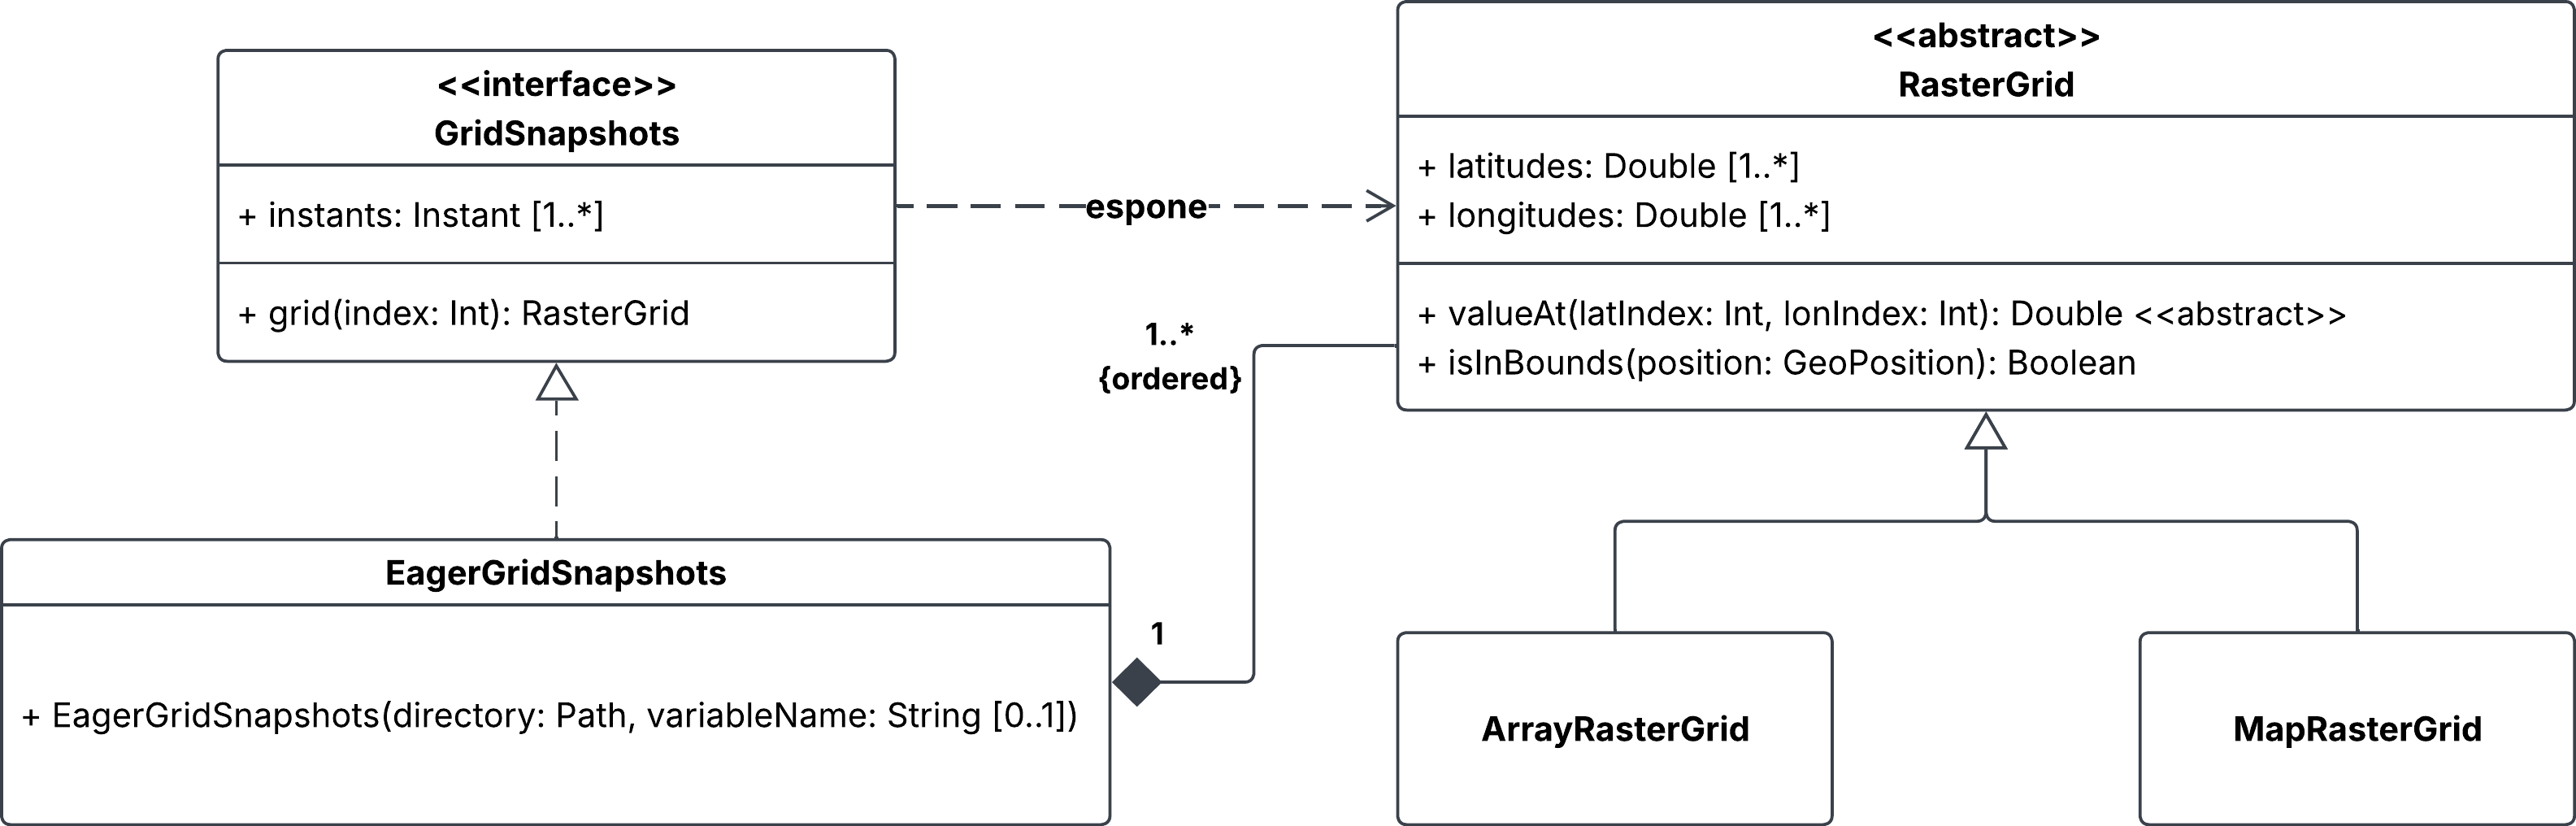
\includegraphics[width=\linewidth]{figures/progettazione/rappresentazione.png}
    \caption[Rappresentazione dei dati raster]{Le astrazioni per una griglia raster e per
    una serie temporale di griglie, con le rispettive realizzazioni.}
    \label{fig:uml-rappresentazione}
\end{figure}

\subsection{La griglia raster}
\label{subsec:raster-grid}

Una griglia raster è definita da due assi indipendenti, di latitudini e di longitudini, e
dai campioni collocati sulle celle che ne risultano. I due assi sono esposti come vettori di
\texttt{Double}; coerentemente con l'ipotesi stabilita nella
Sezione~\ref{subsec:griglie-supportate}, si richiede che siano strettamente monotoni ma non
che siano equispaziati, per cui la posizione di ciascuna coordinata non è ricavabile per via
aritmetica e va conservata esplicitamente. Di conseguenza, l'individuazione della cella che
contiene una data coordinata è una ricerca sull'asse anziché un calcolo.

\texttt{RasterGrid} è una classe astratta e non un'interfaccia. La ragione è che la
validità degli assi, ovvero la loro monotonia stretta, la coerenza fra le loro dimensioni
e il numero dei campioni, è una precondizione che vale per ogni griglia, quale che sia il
modo in cui i campioni siano memorizzati. Collocandone la verifica nel costruttore della
classe astratta, essa viene eseguita per costruzione da ogni realizzazione presente e
futura.

Le due realizzazioni, \texttt{ArrayRasterGrid} e \texttt{MapRasterGrid},
differiscono unicamente nel modo in cui i campioni sono memorizzati, e definiscono
rispettivamente una rappresentazione densa e una sparsa. La distinzione è motivata
dalla variabilità della densità dei dati: una grandezza come la temperatura, campionata
su un'area prevalentemente continentale, riporta una misura in quasi tutte le celle
della griglia; una grandezza come la portata fluviale è invece definita solo lungo i
corsi d'acqua, e lascia priva di misura la maggior parte della griglia.

La scelta fra le due non ricade su chi configura la simulazione: viene effettuata
dinamicamente alla lettura del file, sulla base della densità osservata dei campioni.
Il criterio di scelta è descritto nel Capitolo~\ref{chap:implementazione}.

Si noti che la distinzione è invisibile a chi usa la griglia:
chi vi accede vede unicamente il tipo \texttt{RasterGrid}, e le due realizzazioni
differiscono solo per il compromesso fra memoria occupata e costo di accesso.

\subsection{La serie temporale di griglie}
\label{subsec:grid-snapshots}

\texttt{GridSnapshots} descrive una successione di griglie omogenee, ciascuna associata a
un istante del mondo reale. L'astrazione espone due sole caratteristiche: la successione
ordinata degli istanti e l'accesso alla griglia corrispondente a una data posizione nella
successione. La prima è ciò che consente a chi la interroga di individuare i due istanti
adiacenti a quello richiesto; la seconda, di ottenere le griglie corrispondenti.

La realizzazione fornita, \texttt{EagerGridSnapshots}, costruisce l'intera serie in memoria
al momento della costruzione, leggendo tutti i file presenti in una cartella. La scelta
risponde a \req{NF8}: spostando l'intero accesso al file system nella fase di costruzione,
ogni successiva lettura del layer opera su entità già residenti in memoria, con un costo
indipendente dal formato di origine e dal numero di file da cui la serie è stata ricavata.
La stessa scelta soddisfa \req{NF7}, poiché un file illeggibile o incoerente con gli
altri si manifesta al caricamento della simulazione anziché durante l'esecuzione.

Il prezzo è che l'occupazione di memoria cresce con l'estensione della serie e dell'area
geografica di riferimento. Il vincolo è ritenuto accettabile: le richieste sono formulate
dal modellista in funzione della simulazione che intende condurre. L'astrazione
\texttt{GridSnapshots} non impone comunque questa strategia, e una realizzazione che
carichi le griglie su richiesta è possibile senza alcuna modifica al layer.

Un \ac{GRIB} o \ac{NetCDF} può contenere più variabili distinte: un archivio scaricato da
un data store Copernicus può includere, ad esempio, sia la temperatura a due metri dal suolo
sia la velocità del vento nello stesso file. La costruzione di una serie richiede quindi di specificare
anche quale fra le variabili presenti debba essere estratta. Il nome della variabile può
essere omesso quando i file ne contengono una sola, caso in cui essa è individuata
senza ambiguità.
Il modo in cui una variabile viene individuata ed estratta da un file è discusso nel
Capitolo~\ref{chap:implementazione}. \textbf{\emph{(Capitolo di implementazione)}}

\section{Le strategie di risoluzione dei valori}
\label{sec:risoluzione}

La Sezione~\ref{subsec:discretezza-campioni} ha stabilito, con \req{F5}, che la regola con
cui un valore viene prodotto a partire dai campioni disponibili non può essere fissata nel
codice, ma deve essere configurabile e intercambiabile. Questa sezione ne descrive la
realizzazione come famiglia di strategie, e la estende al secondo passaggio necessario a
produrre il valore restituito dal layer: la traduzione da un \texttt{Double} al tipo
esposto ai nodi, richiesta da \req{F6}.

\subsection{Le strategie di interpolazione}
\label{subsec:interpolazione}

Il requisito si traduce nell'introduzione di un'astrazione per la regola e di
un insieme di realizzazioni intercambiabili, secondo lo schema noto come \emph{strategia}.
La \Cref{fig:uml-interpolazione} riporta la gerarchia risultante.

\begin{figure}[h]
    \centering
    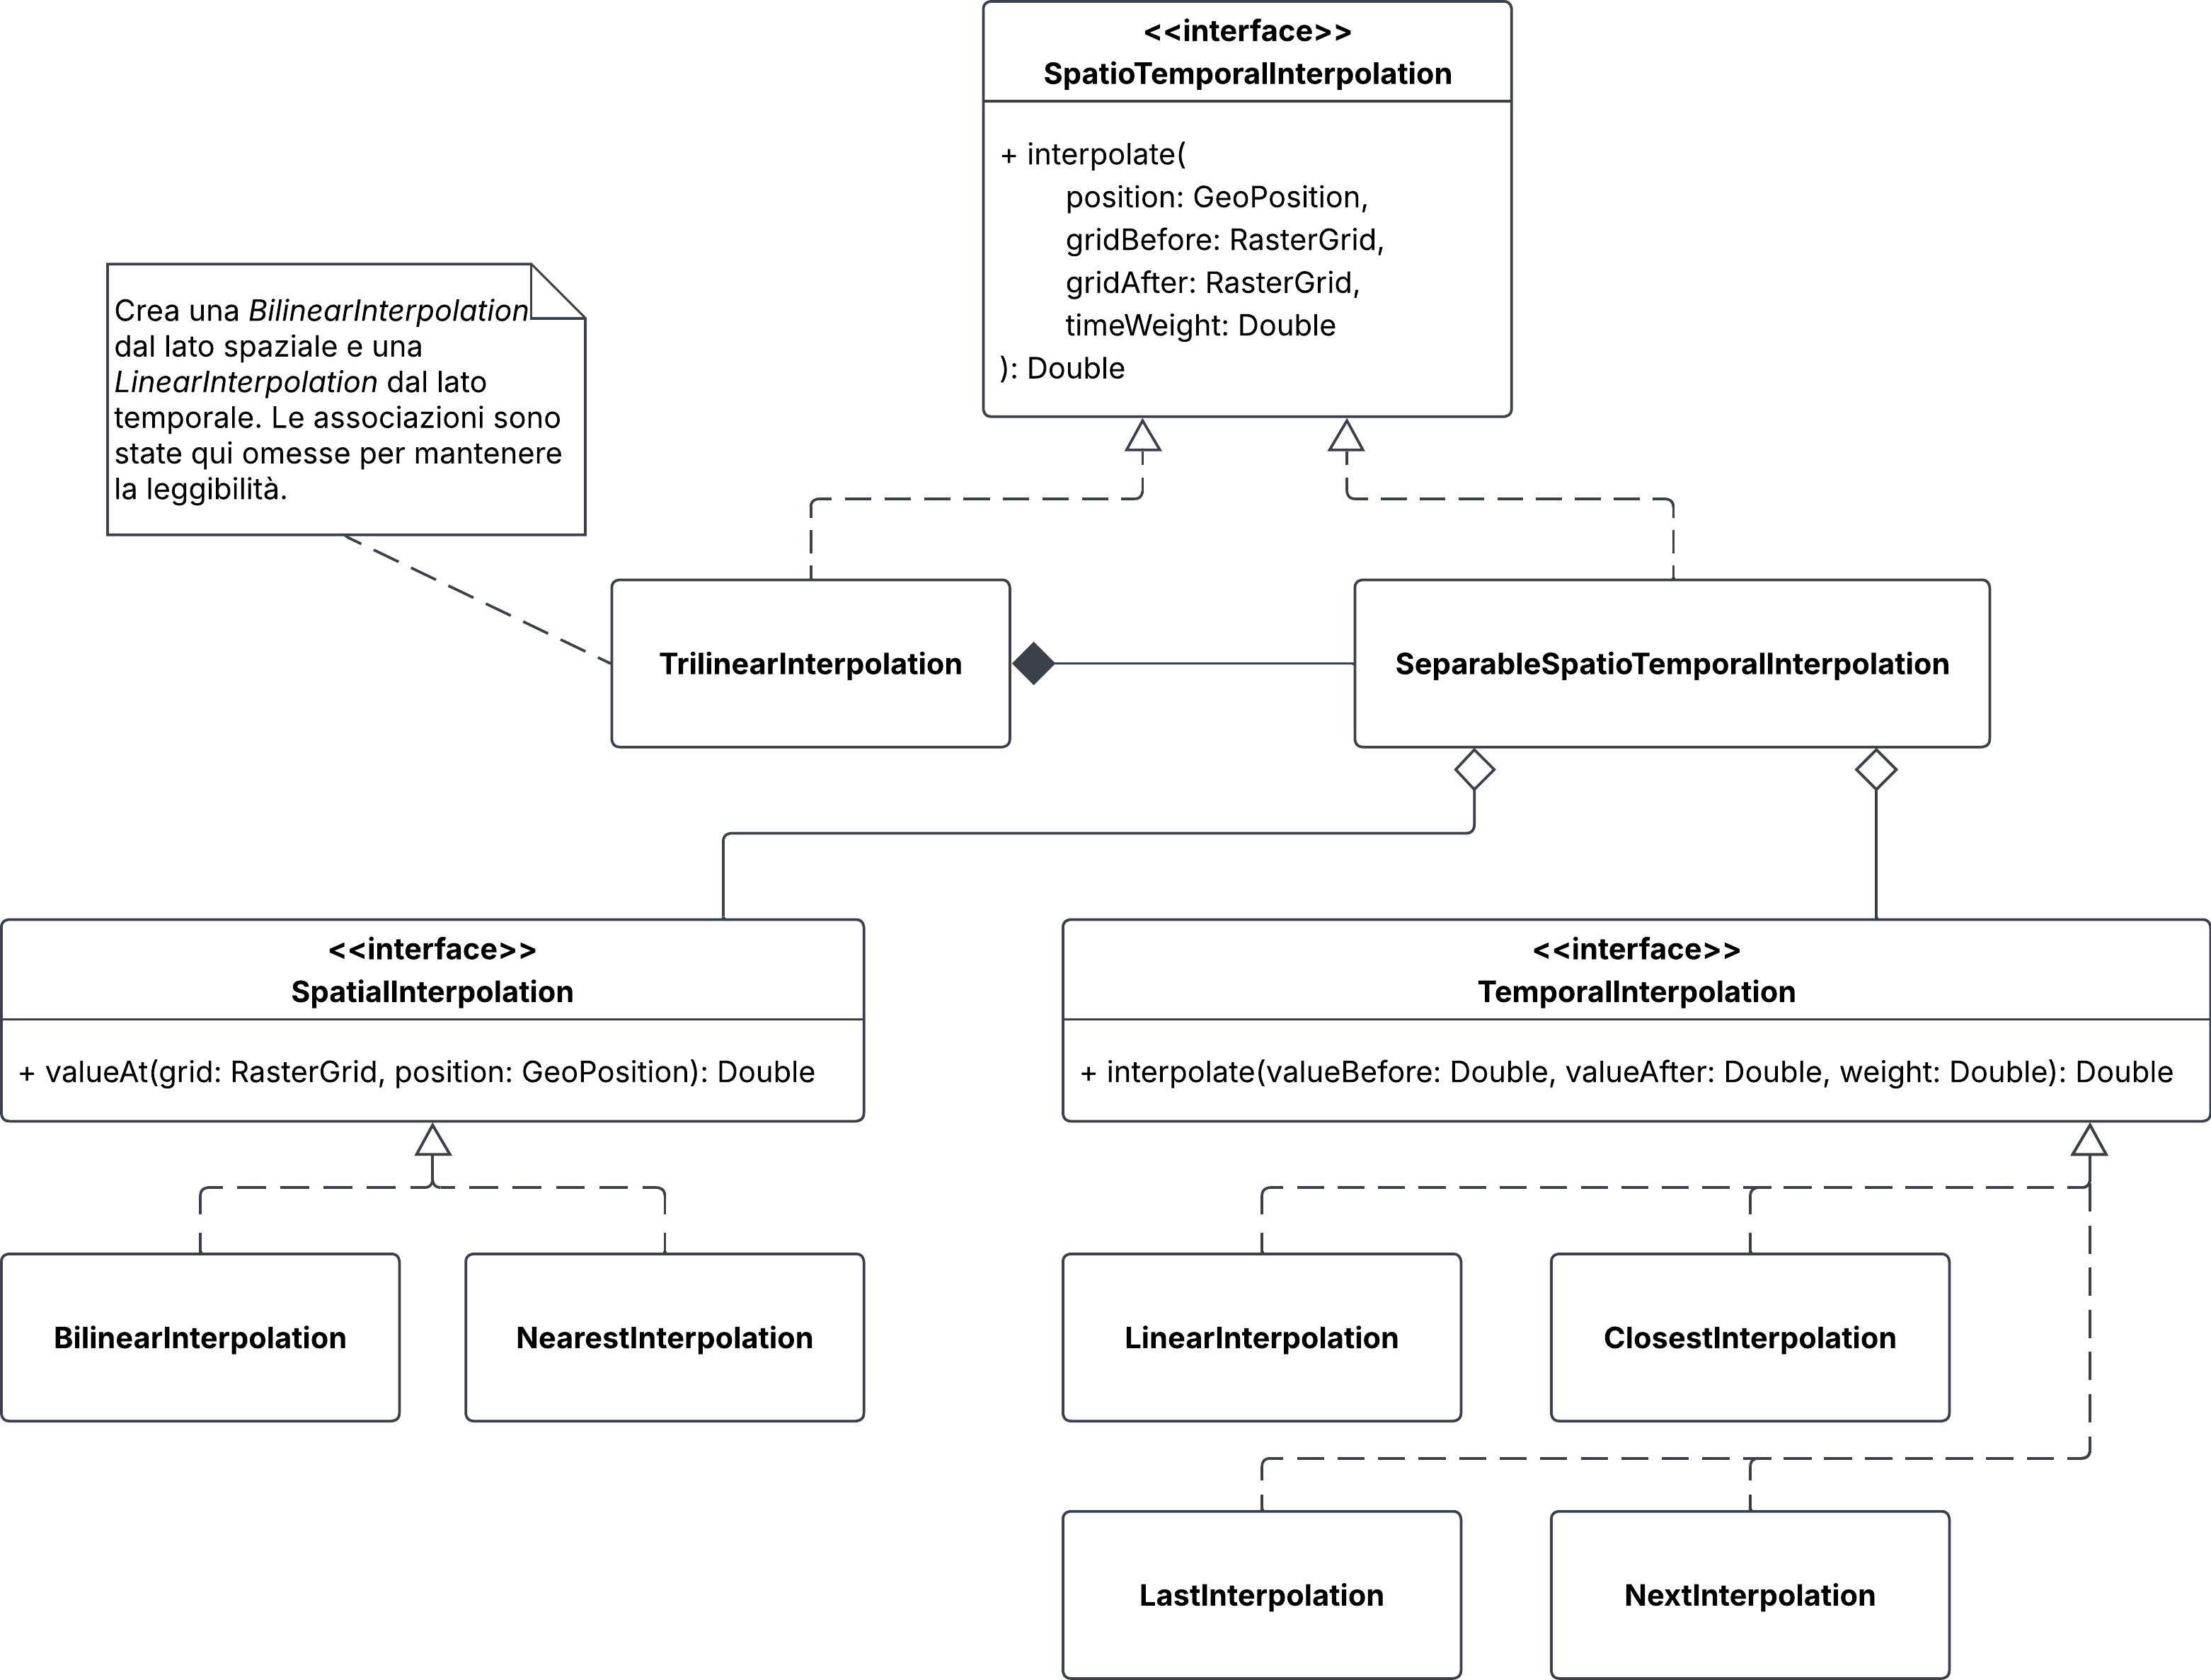
\includegraphics[width=\linewidth]{figures/progettazione/interpolazione.png}
    \caption[Strategie di interpolazione]{Le strategie di interpolazione spaziale,
    temporale e spazio-temporale, e la loro composizione.}
    \label{fig:uml-interpolazione}
\end{figure}

L'astrazione principale, \texttt{SpatioTemporalInterpolation}, attraversa entrambi i
domini: riceve la posizione geografica, due griglie adiacenti all'istante richiesto e
il peso che colloca l'istante richiesto fra i due, e ne produce un valore. La ragione per
cui la regola è espressa da un'unica astrazione anziché da due composte in un ordine
fissato è che non tutte le regole concepibili sono separabili spazialmente e temporalmente: una regola
che consideri contemporaneamente i campioni delle due griglie, senza risolvere prima lo spazio
e poi il tempo, non sarebbe esprimibile.

Altre regole di interesse pratico però sono separabili, ovvero si risolvono collassando
le due griglie spaziali ciascuna a un unico valore in funzione della sola posizione,
per poi decidere il valore finale rispetto alla regola di interpolazione temporale su questi.

Per queste regole, il
modulo introduce \sloppypar{\texttt{SeparableSpatioTemporalInterpolation}}, che realizza l'astrazione
principale componendo due strategie indipendenti: una spaziale, che risolve la posizione
su ciascuna delle due griglie, e una temporale, che combina i due valori così ottenuti
secondo il peso.

Le realizzazioni fornite permettono di distinguere fra grandezze che ammettono valori intermedi e
grandezze che non li ammettono. Sul dominio spaziale, \texttt{BilinearInterpolation}
produce una media pesata dei quattro campioni che circondano la posizione (si veda come riferimento la \Cref{fig:spatial-interp}), adatta a
grandezze continue, mentre \texttt{NearestInterpolation} seleziona il campione della cella
più vicina, scelta ammissibile per grandezze categoriche. Sul dominio temporale,
\texttt{LinearInterpolation} combina i due campioni in proporzione al peso, mentre
\texttt{ClosestInterpolation}, \texttt{LastInterpolation} e \texttt{NextInterpolation} ne
selezionano uno soltanto, rispettivamente il più vicino, il precedente o il successivo.

Fra le combinazioni possibili, una configurazione sufficientemente ricorrente da meritare
un nome proprio, in modo da poter essere istanziata direttamente tramite YAML, è la \texttt{TrilinearInterpolation}.
Essa può essere ottenuta applicando un'interpolazione bilineare sulle due dimensioni spaziali
e una successiva interpolazione lineare lungo quella temporale~\cite{engel2006realtime}.
Quest'ultima non costituisce tuttavia una specializzazione della composizione separabile,
bensì una sua configurazione fissata, e viene quindi realizzata per delegazione.

La strategia di interpolazione è inoltre il punto in cui si decide il destino dei valori
mancanti, qui rappresentati da \texttt{Double.NaN}: \req{F7} ne impone un trattamento
esplicito, e la Sezione~\ref{subsec:discretezza-campioni} ha stabilito che la decisione
dipenda dalla semantica del dato. In \texttt{BilinearInterpolation}, ad esempio, si è
scelto di propagare il valore mancante se almeno uno dei quattro campioni circondanti la
posizione non è presente, e viene allo stesso modo propagato da
\texttt{LinearInterpolation} se uno dei due valori spazialmente risolti è assente.

La verifica che la posizione richiesta ricada entro l'estensione coperta dalle
griglie è compito del layer, e precede l'invocazione della strategia.
Le realizzazioni possono quindi assumere che gli argomenti ricevuti siano ammissibili,
e concentrarsi sulla sola regola di combinazione dei campioni.

\subsection{La conversione del valore}
\label{subsec:conversione}

Risolto il valore numerico, resta il passaggio finale: tradurlo nel tipo esposto dal layer.

\begin{figure}[H]
    \centering
    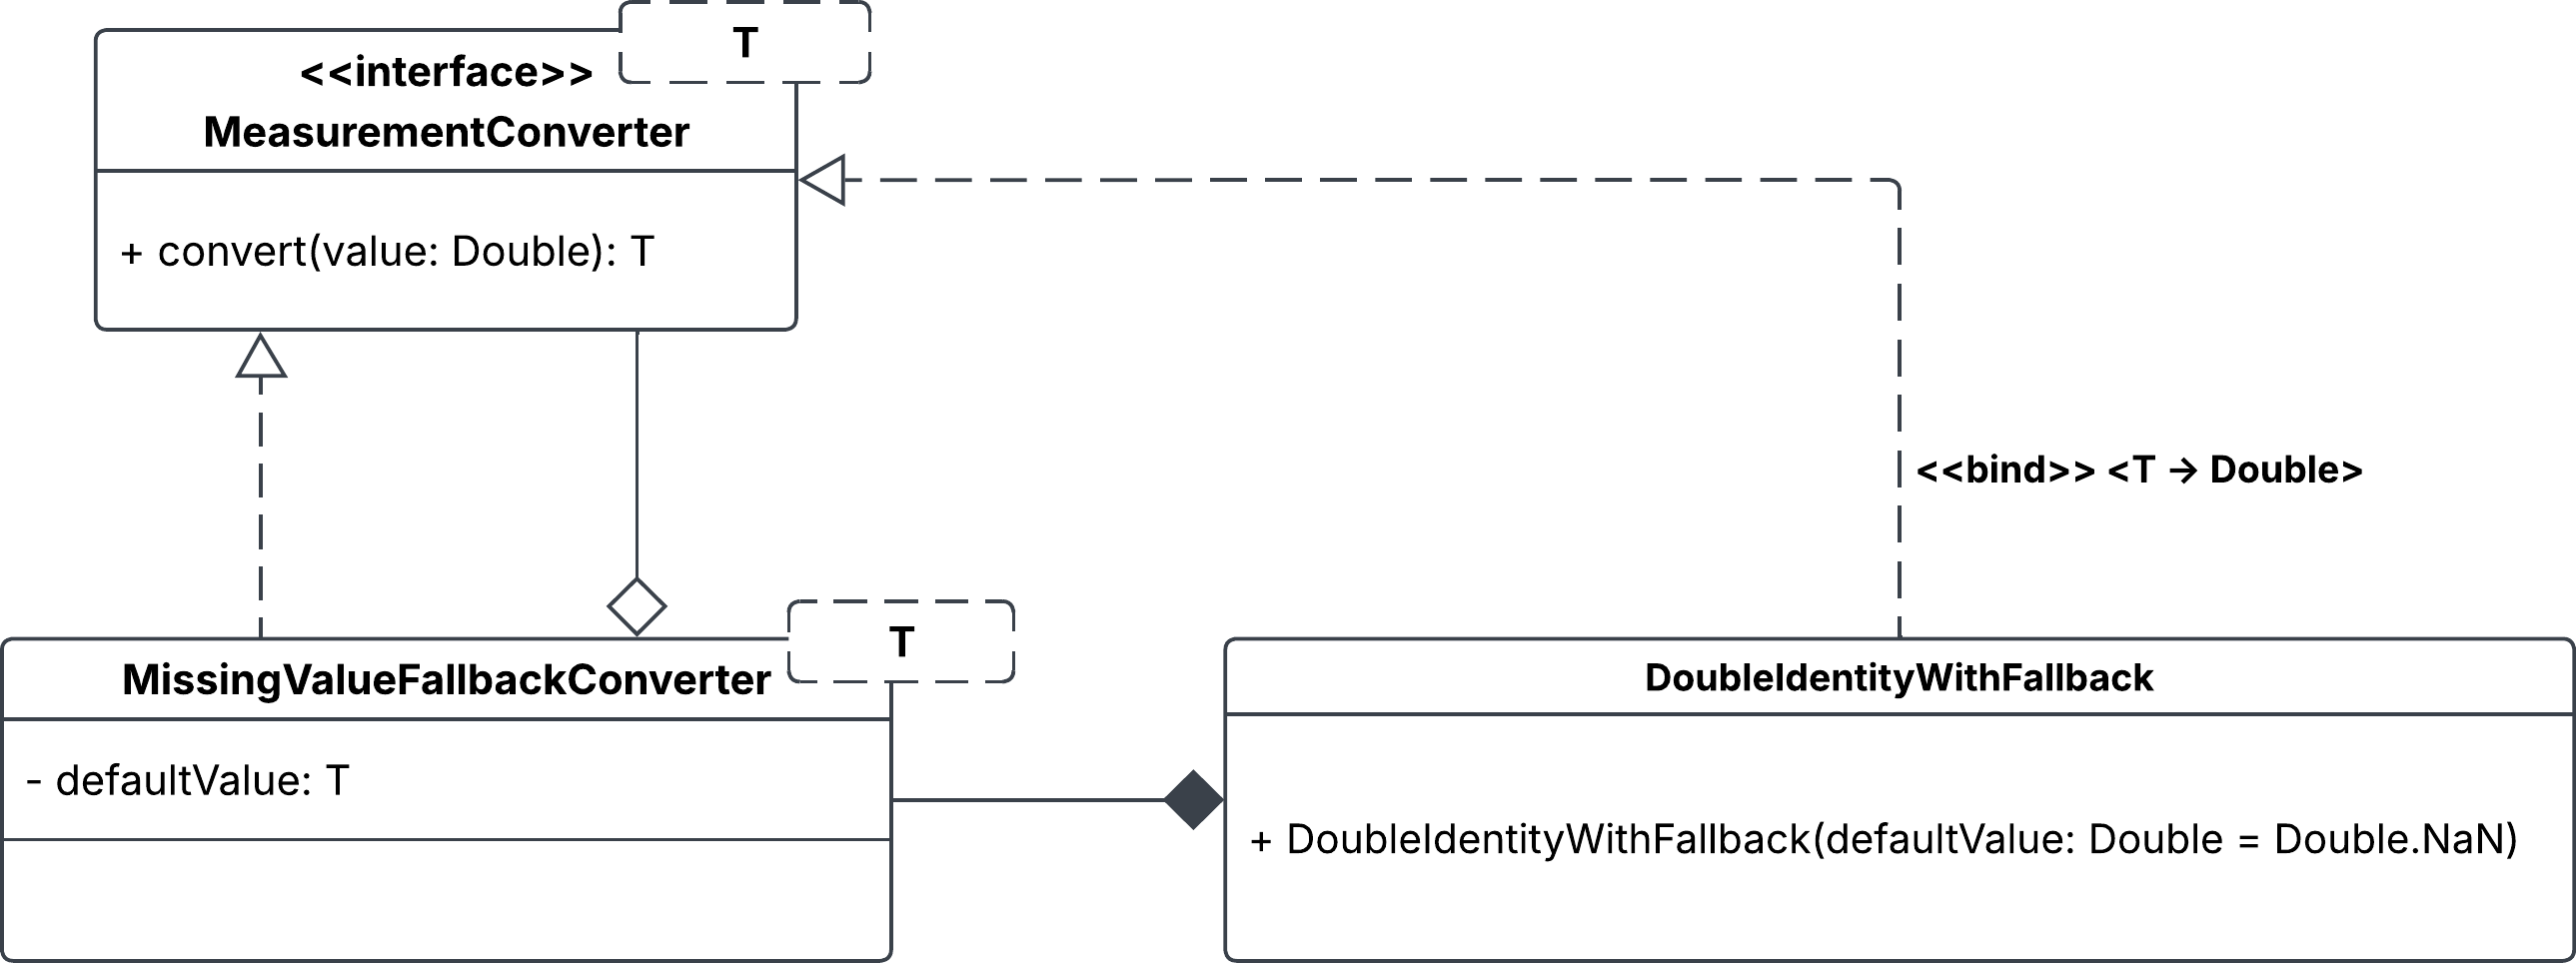
\includegraphics[width=\linewidth]{figures/progettazione/conversione.png}
    \caption[Conversione del valore]{L'astrazione per la conversione del valore risolto e
    la sua composizione con la gestione dei valori mancanti.}
    \label{fig:uml-conversione}
\end{figure}

\texttt{MeasurementConverter<T>} descrive la traduzione da un \texttt{Double} al
tipo \texttt{T} esposto dal layer. È l'unica astrazione del modulo che decide quel tipo,
ed è ciò che soddisfa \req{F6}, consentendo di esporre ai nodi grandezze
la cui interpretazione non è quantitativa, come ad esempio convertendo una soglia in un
valore booleano.

La conversione porta con sé un secondo compito: decidere cosa fare quando il valore
risolto è mancante.
Una scelta che può essere comune nelle simulazioni è poter convertire i valori mancanti
in un valore prefissato, ed è ciò di cui si occupa
\texttt{MissingValueFallbackConverter<T>}, un decoratore che riceve un altro convertitore e un valore di
ripiego: intercetta il caso mancante e restituisce il ripiego, inoltrando ogni altro
valore al convertitore delegato.

\texttt{DoubleIdentityWithFallback} è la configurazione corrispondente al caso più comune,
ovvero un layer che espone direttamente il valore numerico, agendo da funzione identità,
con un possibile ripiego su un valore prestabilito nel caso il dato sia mancante
(propagando il valore assente, se non specificato altrimenti).
Come per \texttt{TrilinearInterpolation}, il suo comportamento viene delegato
poiché è una configurazione fissata a cui si dà un nome, e non una specializzazione della logica.

\section{Il layer Copernicus}
\label{sec:layer}

Il layer è il punto in cui i sottomoduli precedenti vengono composti. La
\Cref{fig:aggr-layer} ne riporta le entità con cui collabora.

\begin{figure}[h]
    \centering
    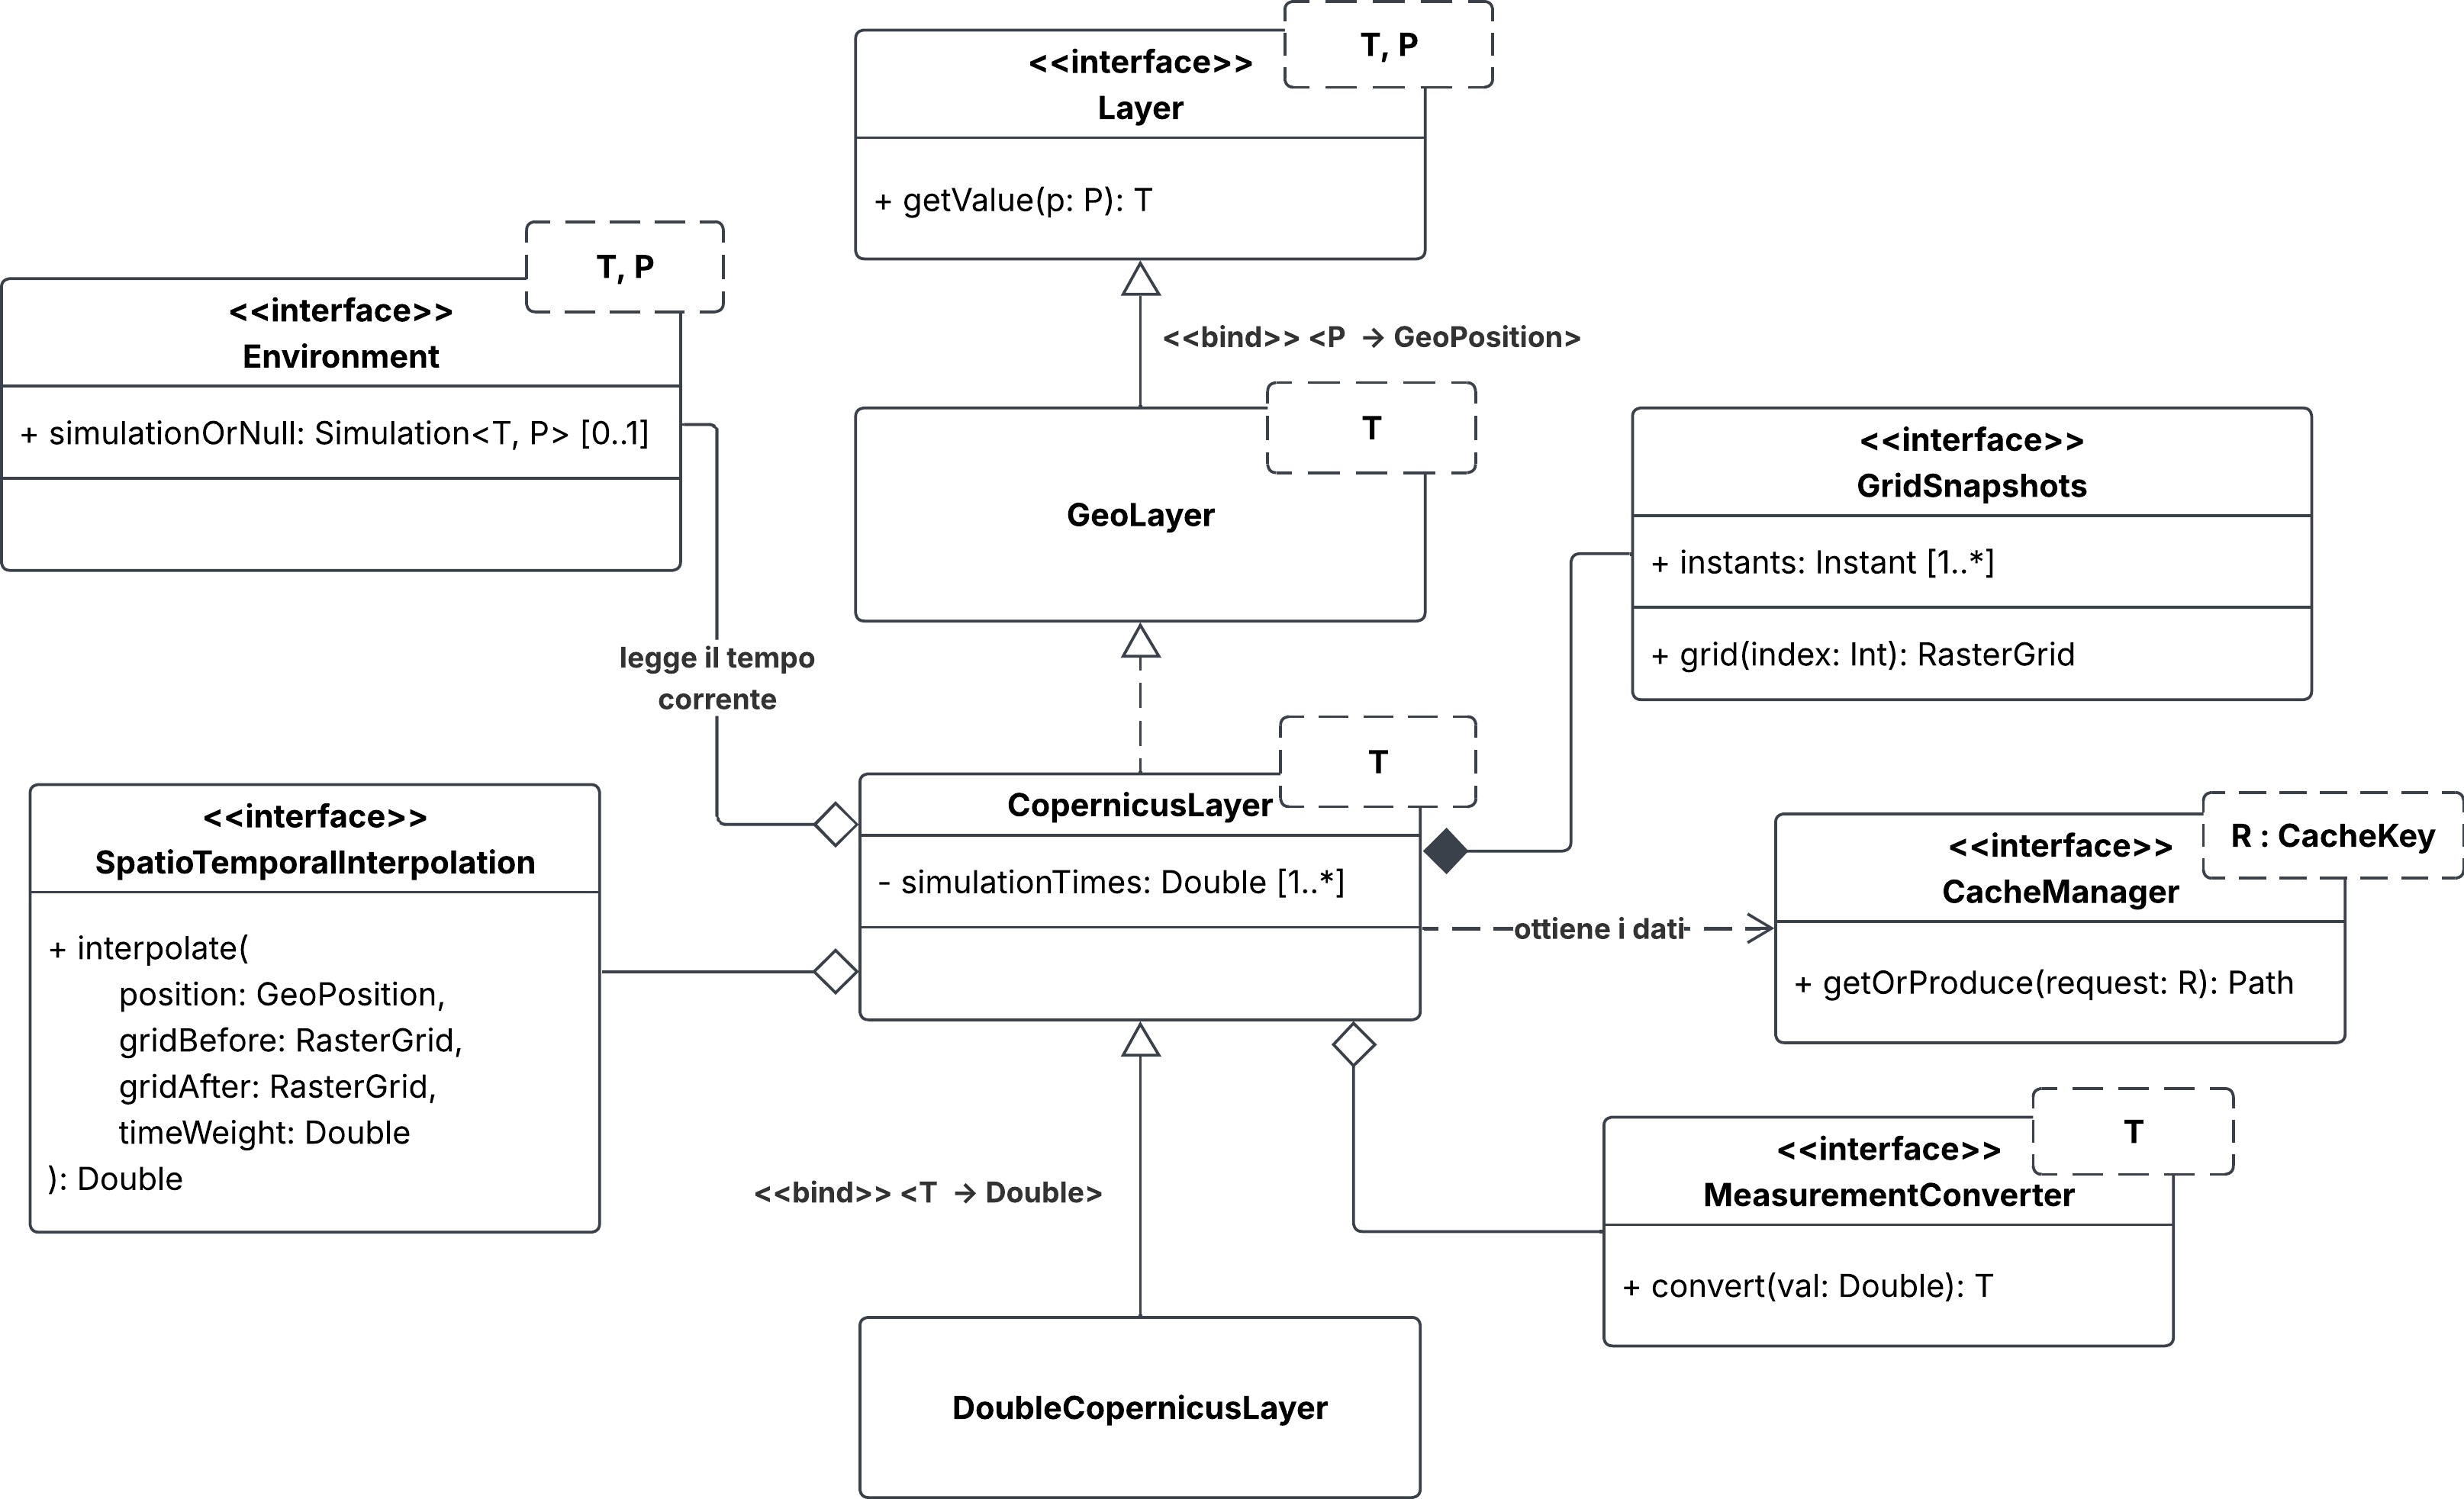
\includegraphics[width=\linewidth]{figures/progettazione/aggr_layer.png}
    \caption[Il layer Copernicus]{La gerarchia del layer e le sue collaborazioni.}
    \label{fig:aggr-layer}
\end{figure}

\subsection{La semantica di interrogazione}
\label{subsec:layer-pull-based}

Il requisito \req{F2} chiede che il valore restituito sia quello percepito all'istante di
simulazione corrente. Perché ciò accada, il layer deve in qualche modo venire a conoscenza
dell'avanzamento del tempo di simulazione, e sono possibili due semantiche opposte.

La prima affida a una reazione dedicata il compito di avanzare esplicitamente lo stato del
layer, in sincronia con l'avanzamento del tempo: a ogni esecuzione, la reazione
aggiornerebbe lo stato corrente esposto dal layer, che si limiterebbe poi a restituirlo.
La seconda non prevede alcuno stato temporale nel layer: quando interrogato, esso legge
autonomamente il tempo di simulazione corrente dall'environment
(Sezione~\ref{subsec:alchemist-time}) e ne ricava il valore.

Il modulo adotta la seconda, per due ragioni:
\begin{itemize}
    \item la prima è di ridondanza: il nodo che interroga il layer vive già
    nell'environment e ne condivide la stessa percezione del tempo, per cui usare una
    reazione dedicata al solo scopo di rendere noto al layer che il tempo è avanzato
    duplicherebbe un'informazione già accessibile al momento della lettura;
    \item la seconda è di determinismo: con una reazione dedicata, il valore letto a un dato
    istante dipenderebbe dall'ordine con cui il motore di simulazione esegue la reazione di
    avanzamento e quella che legge il layer; la semantica a interrogazione elimina il
    problema alla radice, non essendoci alcuno stato da sincronizzare.
\end{itemize}

Per le stesse ragioni, il progetto non introduce un'interfaccia dedicata che aggiunga il
concetto di layer temporale: un layer per dati Copernicus è un'implementazione di
\texttt{Layer<T, GeoPosition>} come un'altra, e non un tipo concettualmente distinto.

\iffalse
\subsection{La corrispondenza temporale}
\label{subsec:layer-corrispondenza}

Letto il tempo di simulazione corrente, il layer deve stabilire a quale istante del mondo
reale esso corrisponda. La Sezione~\ref{subsec:corrispondenza-temporale} ha stabilito che
tale corrispondenza vada confinata nel solo componente che ne ha bisogno, ed è quindi il
layer a ospitarla.

La corrispondenza è definita da due soli parametri: un'\emph{origine}, l'istante reale a
cui corrisponde lo zero del tempo di simulazione, e una \emph{scala}, la durata reale
rappresentata da un'unità di tempo simulato. Fissati questi due valori, ogni istante di
simulazione individua un istante reale e viceversa. Entrambi sono dichiarati da chi
configura la simulazione, come \req{F3} richiede, e restano costanti per l'intera
esecuzione.

L'origine ammette un valore predefinito, ovvero il primo istante coperto dalla
serie, che corrisponde al caso più frequente di una simulazione che inizia
con i dati di cui dispone.

La corrispondenza è stabilita una sola volta, al momento della costruzione del layer, e non
è nota ad alcun'altra parte del simulatore, che continua a operare su un tempo scalare. Ne
consegue che le modifiche richieste da un'eventuale futura migrazione del tipo di tempo di
Alchemist resterebbero circoscritte a un unico punto del modulo.

Ottenuto l'istante reale, resta il caso in cui esso ricada al di fuori dell'intervallo
coperto dalla serie, che la Sezione~\ref{subsec:estensione-spaziale} ha stabilito non
costituire un errore di modellazione. Il layer estrapola a valore costante: se l'istante
precede il primo disponibile viene considerato quest'ultimo, e analogamente, se supera
l'ultimo, viene considerato l'ultimo istante presente nei dati.
\fi
\subsection{La corrispondenza temporale}
\label{sec:corrispondenza-temporale}

Il layer deve mettere in relazione due domini temporali di natura diversa: il tempo
di simulazione, che legge dall'environment quando viene interrogato, e gli istanti
del mondo reale a cui sono riferite le griglie della serie che espone. La
Sezione~\ref{subsec:corrispondenza-temporale} ha stabilito che tale corrispondenza vada
confinata nel solo componente che ne ha bisogno, ed è quindi il layer a ospitarla.

La corrispondenza è definita da due soli parametri: un'\emph{origine}, l'istante
reale a cui corrisponde lo zero del tempo di simulazione, e una \emph{scala}, la
durata reale rappresentata da un'unità di tempo simulato. Fissati questi due valori,
ogni istante di simulazione individua un istante reale e viceversa. Entrambi sono
dichiarati da chi configura la simulazione, come \req{F3} richiede, e restano
costanti per l'intera esecuzione. L'origine ammette un valore predefinito, il primo
istante coperto dalla serie, che corrisponde al caso più frequente di una
simulazione che inizia con i dati di cui dispone.

Essendo la corrispondenza biunivoca, essa può essere applicata in due
direzioni opposte: tradurre a ogni interrogazione il tempo di simulazione corrente
nell'istante reale che gli corrisponde, oppure tradurre una volta sola l'intera
successione degli istanti della serie in tempi di simulazione. Il modulo adotta la
seconda: alla costruzione del layer l'asse temporale della serie viene ricondotto al
tempo di simulazione, e il layer conserva la successione così ottenuta in un
vettore di scalari.

La scelta fa della costruzione l'unico punto in cui i due domini si incontrano.
Tutto ciò che avviene durante l'esecuzione, ovvero l'individuazione dei due campioni
che racchiudono l'istante richiesto, il calcolo del peso temporale e il trattamento
degli istanti esterni all'intervallo coperto, opera tramite
il valore letto dall'environment.

La conversione è ospitata dal layer e non dalla serie di griglie. Questo perché
\texttt{GridSnapshots} descrive dati, non una simulazione, e i suoi istanti
restano quelli del mondo reale a cui le griglie sono riferite, indipendentemente da
quale simulazione li utilizzi e con quale convenzione.

Resta il caso in cui il tempo di simulazione corrente ricada al di fuori
dell'intervallo coperto dall'asse così ottenuto, che la
Sezione~\ref{subsec:estensione-spaziale} ha stabilito non costituire un errore di
modellazione. Il layer estrapola a valore costante: se l'istante richiesto precede
il primo disponibile viene considerato quest'ultimo e, analogamente, se supera
l'ultimo viene considerato l'ultimo presente nei dati.

Poiché la corrispondenza è stabilita una sola volta, alla costruzione, e non è nota
ad alcun'altra parte del simulatore, che continua a operare su un tempo scalare, le
modifiche richieste da un'eventuale futura migrazione del tipo di tempo di Alchemist
resterebbero circoscritte a un unico punto del modulo.

\subsection{Collocazione nella gerarchia e responsabilità}
\label{subsec:layer-gerarchia}

Fra l'interfaccia \texttt{Layer<T, P>} di Alchemist e la realizzazione concreta è
interposta \texttt{GeoLayer<T>}, che fissa il tipo delle posizioni a \texttt{GeoPosition}
lasciando libero il tipo del valore esposto. L'astrazione intermedia non aggiunge alcun
metodo: il suo scopo è dare un nome alla specializzazione geospaziale del layer.

\texttt{CopernicusLayer<T>} realizza tale astrazione, e le sue responsabilità sono tutte di
coordinamento: individuare le griglie pertinenti al momento in cui viene interrogato e
delegare alle strategie la produzione del valore. Il layer non contiene alcuna logica di
interpolazione né alcuna conoscenza dei formati di origine: è il luogo in cui le decisioni
prese altrove vengono applicate nell'ordine corretto.

La \Cref{fig:layer-sequenza} riporta la distribuzione delle responsabilità fra il layer e 
le entità con cui interagisce nel corso di una singola interrogazione.

\begin{figure}[H]
    \centering
    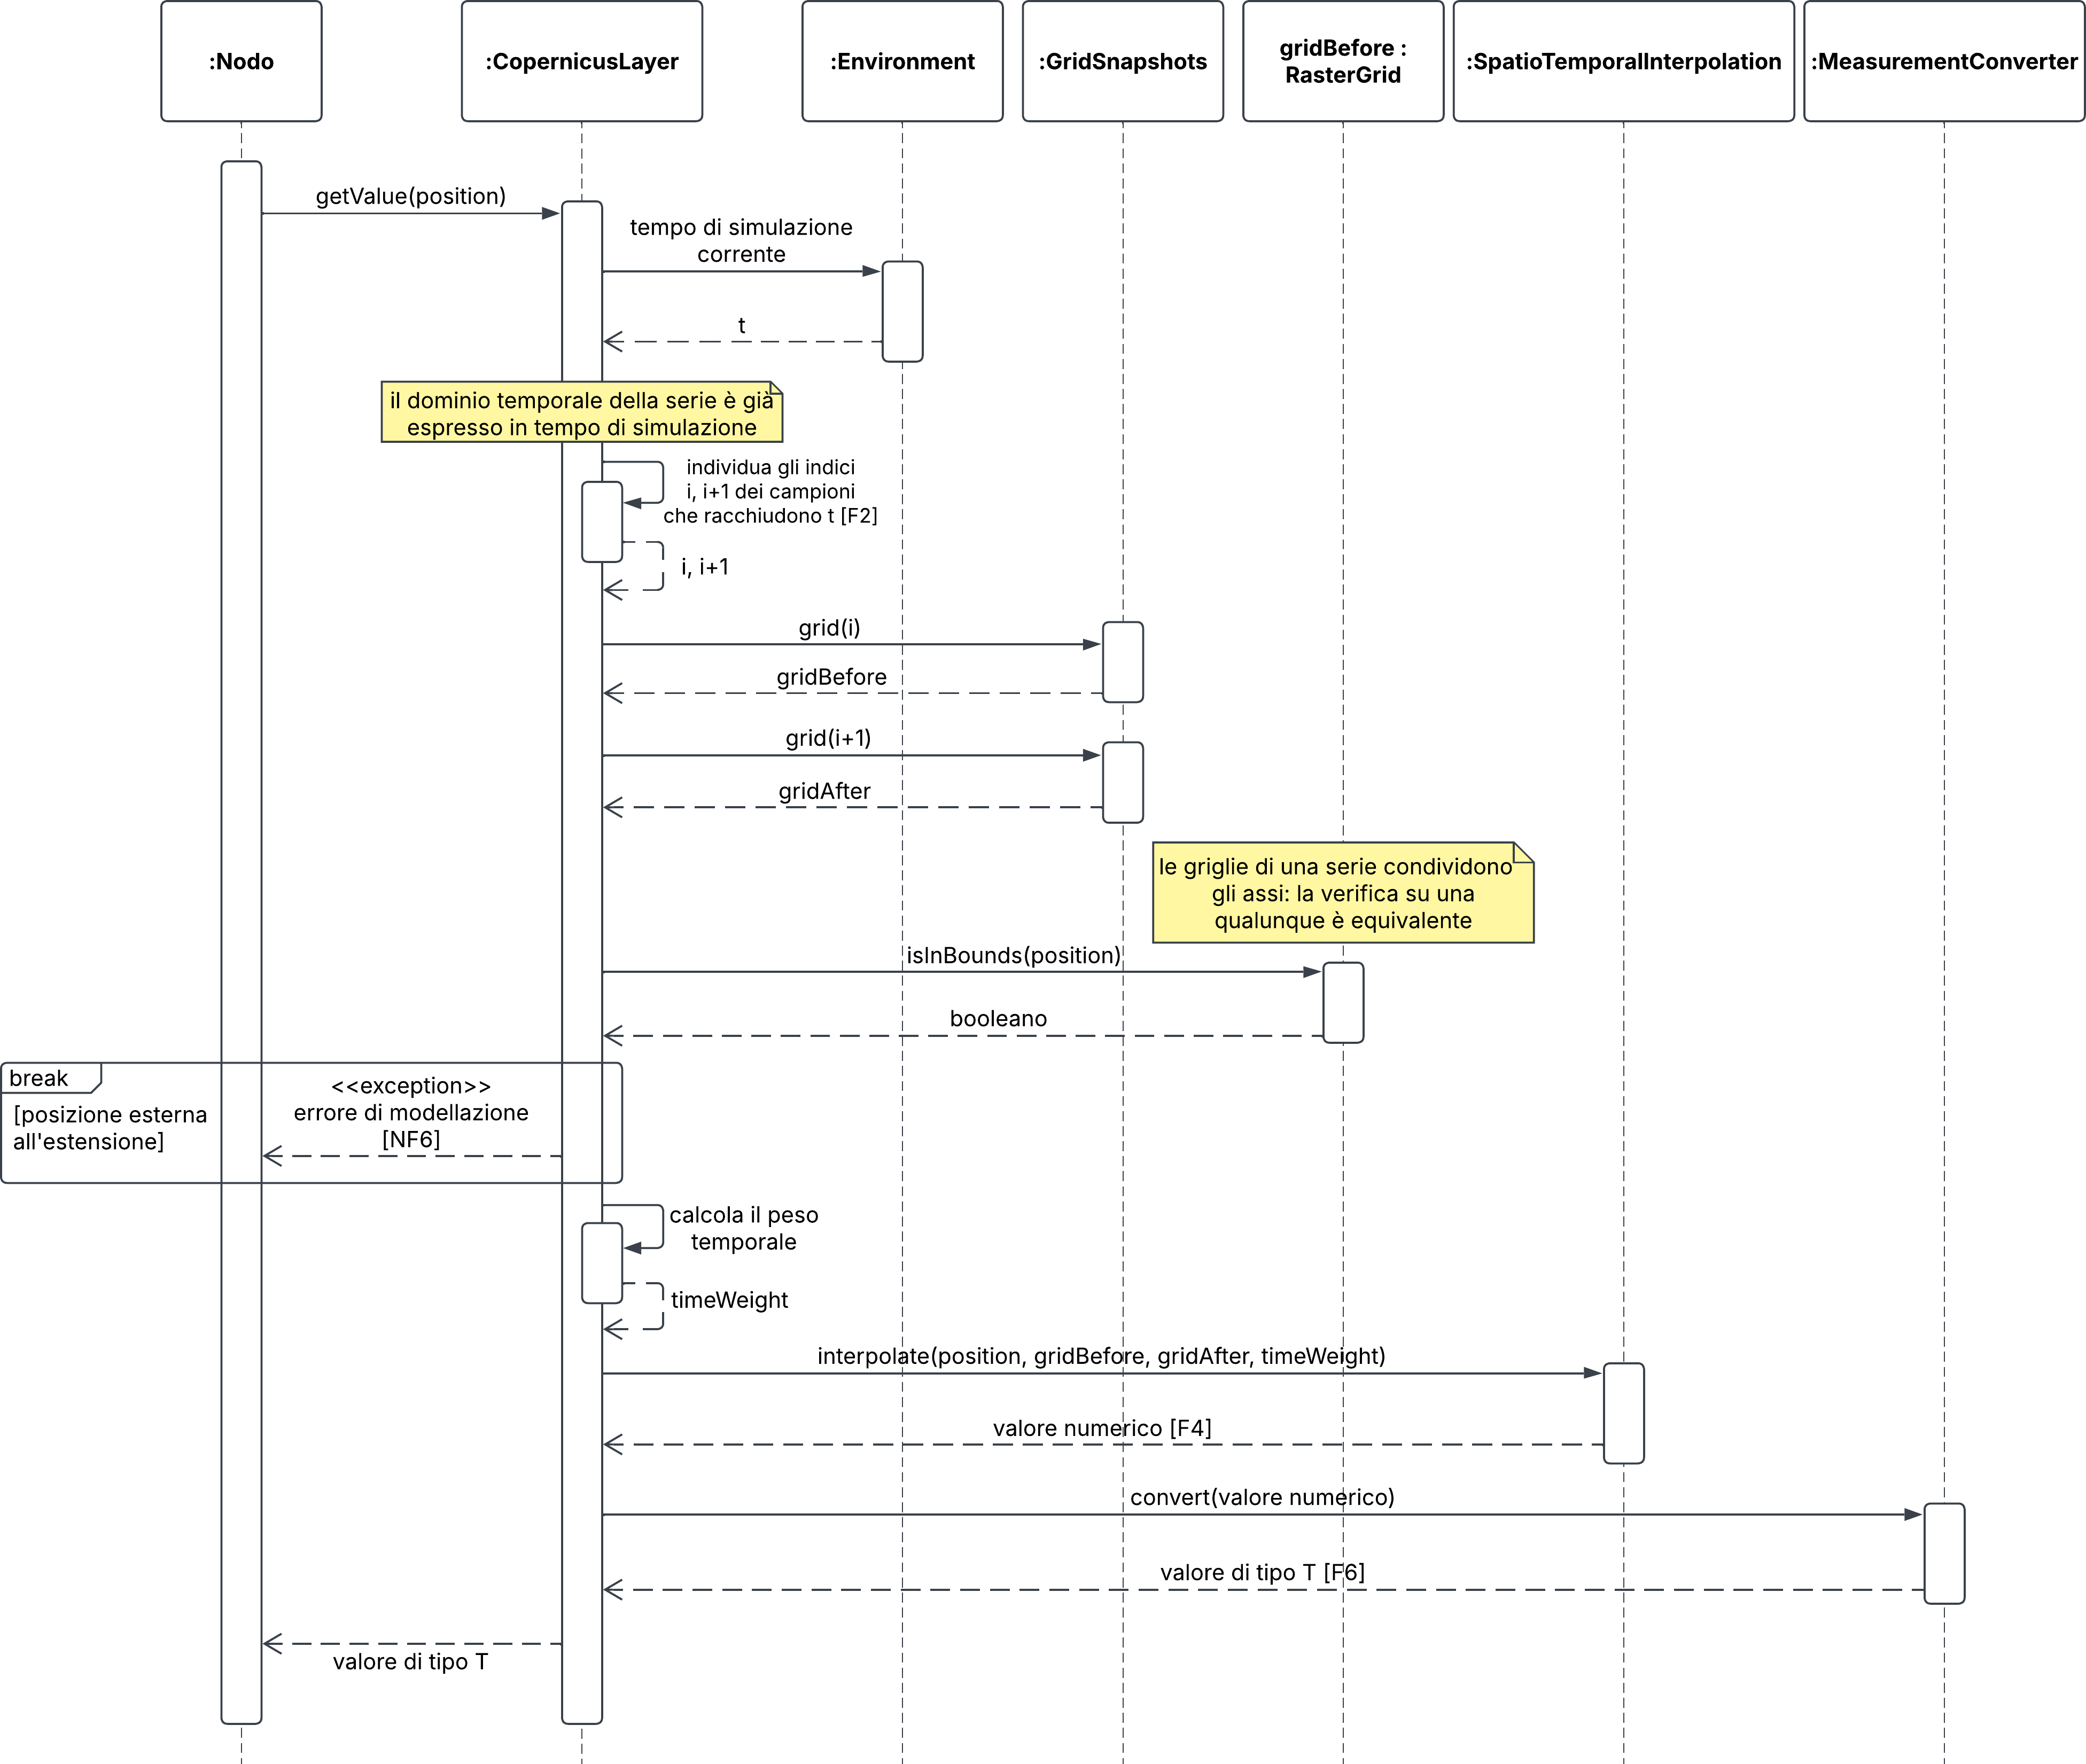
\includegraphics[width=\linewidth]{figures/progettazione/sequenza_layer.png}
    \caption[Interrogazione del layer]{Le interazioni fra il layer e le entità con cui collabora quando gli viene richiesto un valore.}
    \label{fig:layer-sequenza}
\end{figure}

La lettura del tempo di simulazione dall'environment attua la semantica discussa nella
Sezione~\ref{subsec:layer-pull-based}: è il layer a procurarselo al momento
dell'interrogazione, e non un evento esterno a comunicarglielo. L'istante così ottenuto
viene ricondotto al dominio temporale dei dati secondo la corrispondenza fissata alla
costruzione, individuando i due campioni
temporali che lo racchiudono e, con essi, le griglie corrispondenti (\req{F3}).

Disponendo delle griglie, il layer può verificare che la posizione richiesta ricada nella
regione da esse coperta. La verifica attua la delimitazione stabilita nella
Sezione~\ref{subsec:estensione-spaziale}: una posizione esterna non individua alcuna
misura, e la richiesta viene respinta anziché produrre un valore plausibile ma infondato
(\req{NF6}).

Superata la verifica, il layer calcola il peso temporale, che esprime la posizione relativa
dell'istante richiesto fra le due griglie nella forma attesa dalla strategia di
interpolazione.

Le due deleghe finali affidano a componenti esterni al layer le decisioni che dipendono
dalla semantica della grandezza esposta: la produzione del valore numerico a partire dai
campioni adiacenti (\req{F4}) e la sua traduzione nel tipo esposto ai nodi (\req{F6}).

Nessuno di questi passi accede a risorse esterne, come \req{NF8} richiede: la serie di
griglie è già residente in memoria, e la corrispondenza temporale è stata fissata alla
costruzione.

\subsection{Le modalità di costruzione}
\label{subsec:layer-costruzione}

Il layer prevede tre modalità di costruzione, ordinate per ampiezza decrescente di ciò che
si assume già disponibile.

\begin{enumerate}
    \item \textbf{Da una serie già disponibile}: il layer riceve direttamente una
    \texttt{GridSnapshots}, senza sapere da dove provenga.
    \item \textbf{Da una cartella locale}: il layer riceve la collocazione di una cartella
    contenente file già presenti sulla macchina, e da essi costruisce la serie.
    \item \textbf{Da un data store remoto}: il layer riceve la descrizione di una richiesta verso un
    data store Copernicus, e ne ottiene una cartella tramite il sottosistema di
    acquisizione (Sezione~\ref{sec:acquisizione}).
\end{enumerate}

Le tre modalità sono stratificate: ciascuna produce l'argomento della precedente,
riducendosi così alla prima. Poiché ciò che le distingue riguarda
esclusivamente il modo in cui la serie viene ottenuta, e non ciò che il layer ne
fa una volta ottenuta, il comportamento del layer è verificabile in isolamento
fornendo direttamente una serie, senza leggere file né accedere alla rete, come
\req{NF4} richiede.

L'ipotesi stabilita nella Sezione~\ref{subsec:griglie-supportate} riguarda la forma della griglia,
ma non la provenienza dei file. Un dataset campionato su una griglia in proiezione
cartografica non è utilizzabile nella forma in cui il data store lo distribuisce,
ma lo diventa una volta ricondotto a una griglia definita da assi indipendenti di
latitudine e longitudine. La costruzione a partire da una cartella locale accoglie anche
questo caso: il file convertito viene letto come qualunque altro.

In tutte e tre le modalità, inoltre, l'acquisizione e la lettura dei dati
avvengono per intero durante la costruzione del layer, ovvero al caricamento
della simulazione: è quindi lì che si manifesta ogni condizione che impedisca
alla simulazione di disporre dei dati di cui ha bisogno, come \req{NF7} richiede. 

La classe \texttt{CopernicusLayer<T>} è generica nel tipo esposto; il modulo fornisce anche
\texttt{DoubleCopernicusLayer}, che ne fissa il parametro al tipo numerico. La sua
esistenza soddisfa \req{F11}: il meccanismo di caricamento delle simulazioni non è in
grado di istanziare una classe generica, mentre può farlo con una sua specializzazione
concreta (Sezione~\ref{subsec:alchemist-loader}). La specializzazione è inoltre il punto in cui i valori predefiniti delle
strategie possono essere stabiliti, cosa non possibile nella classe generica, non essendo
definibile un convertitore predefinito verso un tipo arbitrario.

Il modo in cui vengono definiti i tre costruttori e i valori di default dei loro
argomenti sono discussi nel Capitolo~\ref{chap:implementazione}. \textbf{\emph{(Capitolo di implementazione)}}

\section{Il sottosistema di acquisizione dati}
\label{sec:acquisizione}

L'ultimo sottomodulo risponde al sotto-problema di acquisizione: ottenere i dati da un
servizio remoto in modo riproducibile, senza riscaricarli a ogni esecuzione
(\req{F9}, \req{F10}). La \Cref{fig:uml-acquisizione} ne riporta le astrazioni e le
realizzazioni.

\begin{figure}[H]
    \centering
    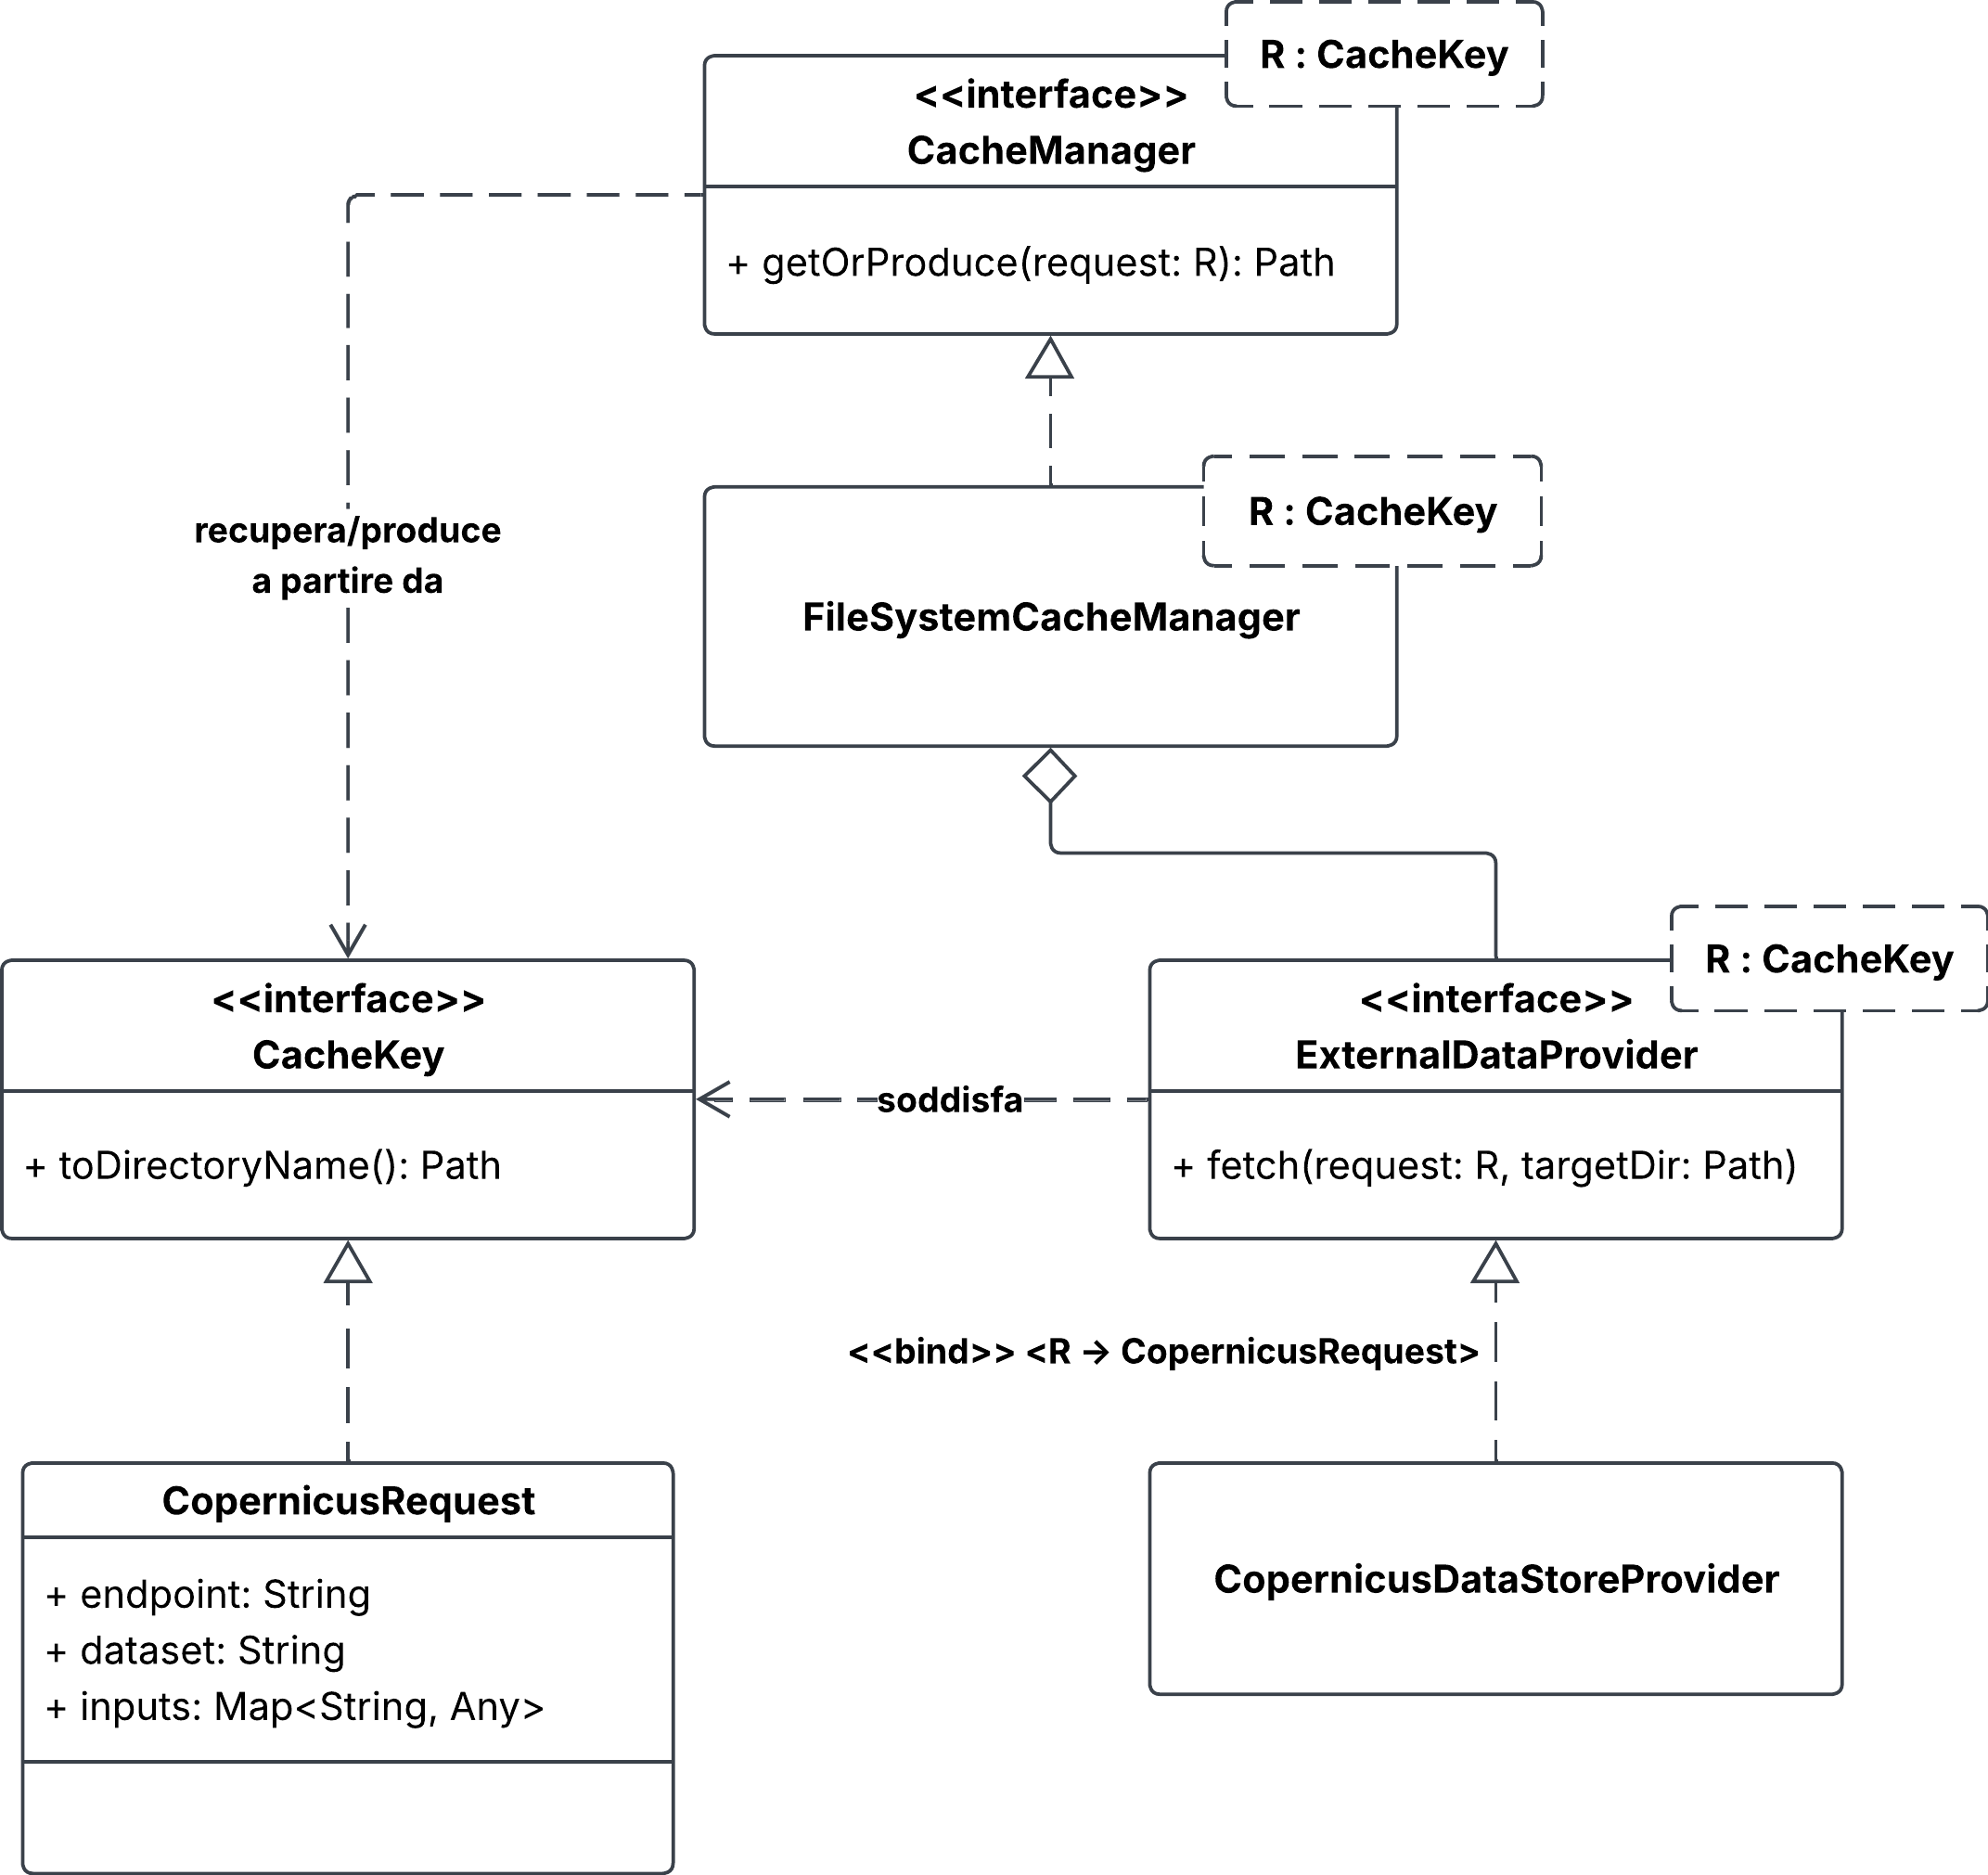
\includegraphics[width=0.9\linewidth]{figures/progettazione/acquisizione.png}
    \caption[Il sottosistema di acquisizione]{Le astrazioni per la cache e per l'accesso a
    fonti esterne, e le realizzazioni relative ai data store Copernicus.}
    \label{fig:uml-acquisizione}
\end{figure}

\subsection{Le astrazioni}
\label{subsec:acquisizione-astrazioni}

Il sottosistema è costruito su tre astrazioni, corrispondenti alle entità individuate nel
modello del dominio:

\begin{itemize}
    \item \texttt{CacheKey}: la descrizione dei dati da ottenere, che ne costituisce
    l'identità. L'unica capacità che l'astrazione richiede è di sapersi tradurre in un nome
    di cartella deterministicamente, in modo tale che descrizioni uguali producano lo stesso nome e
    descrizioni diverse nomi diversi.
    \item \texttt{ExternalDataProvider<R>}: la fonte in grado di soddisfare una
    descrizione, depositando i file corrispondenti in una cartella indicata dal chiamante.
    L'astrazione non indica né il modo né il formato: si limita a stabilire che,
    al termine dell'operazione, la cartella contenga i dati richiesti.
    \item \texttt{CacheManager<R>}: l'entità che, data una descrizione, restituisce la
    cartella contenente i dati corrispondenti, interpellando la fonte esterna solo quando
    non siano già disponibili localmente.
\end{itemize}

Tutte e tre sono parametriche nel tipo della descrizione, vincolato a essere una
\texttt{CacheKey}. Il parametro è ciò che garantisce staticamente che un
gestore di cache e la fonte a cui esso si rivolge accettino la stessa descrizione, senza
che tale coerenza debba essere verificata a tempo di esecuzione.

\subsection{L'indipendenza dalla fonte}
\label{subsec:acquisizione-indipendenza}

Il gestore della cache, \texttt{FileSystemCacheManager<R>}, è indipendente dalla natura della
fonte. Il suo compito consiste nel risolvere il nome della cartella a partire dalla
descrizione, verificarne l'esistenza, e in caso contrario invocare la fonte e conservarne
il risultato nel file system: nessuna di queste operazioni richiede di sapere se i dati
provengano da un data store Copernicus, da un servizio di estrazione cartografica o da
qualunque altra sorgente. Le uniche realizzazioni che conoscono i data store Copernicus
sono \texttt{CopernicusRequest}, che descrive una richiesta verso di essi, e
\texttt{CopernicusDataStoreProvider}, che la soddisfa dialogando con il servizio remoto
secondo il paradigma descritto nella Sezione~\ref{sec:ogc-api-processes}.

È questa suddivisione a rendere effettivo \req{NF2}. In questo modo il sistema
di acquisizione può essere facilmente esteso per supportare altre fonti di dati;
ad esempio, per il recupero
di estratti cartografici da OpenStreetMap, necessario a popolare un
\texttt{OSMEnvironment} (Sezione~\ref{subsec:alchemist-osm}): un servizio di questo tipo
non condivide con i data store Copernicus né il formato dei dati consegnati né il
protocollo con cui la richiesta viene formulata.
Estendere il sottosistema per accoglierlo richiederebbe tuttavia di
realizzare soltanto la coppia \texttt{CacheKey} ed \texttt{ExternalDataProvider<R>}
corrispondente, senza modificare né il gestore della cache né alcuna delle parti già
descritte.

Come il gestore della cache riesce a soddisfare il requisito \req{NF9} è descritto
nel Capitolo~\ref{chap:implementazione}. \textbf{\emph{(Capitolo di implementazione)}}

\subsection{L'identità di una richiesta}
\label{subsec:acquisizione-identita}

Il requisito \req{NF5} chiede che la stessa richiesta corrisponda in modo deterministico
alla stessa voce di cache, ed è ciò che rende possibile \req{F10}. Ciò richiede di
stabilire che cosa costituisca l'identità di una richiesta verso un data store Copernicus,
e come tale identità venga tradotta in un nome di cartella.

L'identità è data dalla terna costituita dal data store interrogato, dal dataset richiesto
e dalla selezione dei parametri con cui la richiesta è stata formulata. Quest'ultima è
deliberatamente non tipizzata: come osservato nella Sezione~\ref{sec:copernicus}, i tre
data store condividono la stessa infrastruttura ma non il catalogo, e ogni dataset ammette
una selezione di parametri propria; imporre una struttura fissa avrebbe limitato
il modulo all'utilizzo di pochi dataset, in contrasto con \req{F8}.

Nel Capitolo~\ref{chap:implementazione} viene discusso come la selezione dei parametri
viene rappresentata e il modo in cui l'identità della richiesta viene tradotta
deterministicamente nel nome di una cartella in cache.

%----------------------------------------------------------------------------------------
% CAPITOLO 5 (IMPLEMENTAZIONE)
%----------------------------------------------------------------------------------------

\chapter{Implementazione}
\label{chap:implementazione}

\iffalse
Questo capitolo descrive come le scelte del Capitolo~\ref{chap:progettazione} sono state
realizzate, seguendone la stessa articolazione. Vengono riportati i soli
punti in cui la realizzazione ha richiesto decisioni non deducibili dalla progettazione,
ovvero quelli in cui il formato dei dati, il protocollo dei servizi remoti o il meccanismo
di caricamento di Alchemist hanno imposto una forma particolare.
\fi

\section{La lettura dei dati}
\label{sec:rappresentazione-impl}

La lettura di \ac{NetCDF} e \ac{GRIB} è delegata alla libreria NetCDF-Java~\cite{netcdfjava},
sviluppata da Unidata. La libreria espone entrambi i formati attraverso lo stesso modello
di dati, il \ac{CDM}, che descrive un file come un insieme di variabili definite su assi
tipizzati (\req{F8}).

I file sono aperti in modalità \emph{enhanced}, nella quale la libreria interpreta i metadati
già presenti nel file per esporre gli assi tipizzati e, soprattutto, sostituisce
automaticamente i valori convenzionali di riempimento con \texttt{Double.NaN}. La
convenzione interna del modulo per i valori mancanti coincide quindi con quella che la
libreria produce.

\iffalse
\subsection{L'accesso ai formati}
\label{subsec:formati-impl}

La lettura di \ac{NetCDF} e \ac{GRIB} è delegata alla libreria NetCDF-Java~\cite{netcdfjava},
sviluppata da Unidata. La libreria espone entrambi i formati attraverso lo stesso modello
di dati, il \ac{CDM}, che descrive un file come un insieme di variabili definite su assi
tipizzati. Questa uniformità rende possibile \req{F8}: il codice del modulo non distingue
fra i due formati.

I file sono aperti in modalità \emph{enhanced}, nella quale la libreria interpreta i metadati
già presenti nel file per esporre gli assi tipizzati e, soprattutto, sostituisce
automaticamente i valori convenzionali di riempimento con \texttt{Double.NaN}. La
convenzione interna del modulo per i valori mancanti coincide quindi con quella che la
libreria produce.

L'apertura dei file \ac{GRIB} ha richiesto un accorgimento aggiuntivo. Questo formato
necessita di tabelle \ac{XML} esterne
per identificare la variabile di riferimento. La libreria NetCDF-Java contiene
già queste tabelle, ma richiede una specifica realizzazione della fabbrica di parser
per poterle leggere, e fallisce se un'altra risulta registrata a livello di sistema.
L'apertura di un file imposta pertanto temporaneamente la proprietà di sistema
corrispondente, ripristinando il valore precedente, o rimuovendolo se assente,
non appena il file è aperto (\Cref{lst:sax-parser}).

\lstinputlisting[
    language=Kotlin,
    label={lst:sax-parser},
    caption={[Gestione del parser per i file GRIB]Apertura di un file con ripristino della fabbrica di parser preesistente.}
]{listings/implementazione/sax-parser.kt}
\fi

\subsection{L'individuazione e la normalizzazione degli assi}
\label{subsec:normalizzazione-impl}

Il \ac{CDM} associa a ogni asse un tipo che ne specifica il ruolo. La lettura si fonda su
questi tipi anziché sui nomi delle dimensioni, che variano da dataset a dataset: lo stesso
asse compare come \texttt{latitude} in alcuni file e come \texttt{lat} in altri, mentre il
tipo dichiarato è in entrambi i casi quello di latitudine.

Sull'asse temporale il tipo dichiarato non è sempre lo stesso: i dataset che distribuiscono
previsioni espongono l'istante di emissione e quello di validità con tipi distinti, e alcuni
archivi etichettano il proprio unico asse temporale come istante di emissione.
Il \Cref{lst:lettura-assi} riporta l'individuazione dei tre assi, ciascuno ottenuto con
\texttt{findCoordinateAxis} a partire dal tipo cercato.

\lstinputlisting[
    language=Kotlin,
    label={lst:lettura-assi},
    caption={[Individuazione degli assi spaziali e temporali]Individuazione degli assi a partire dal tipo dichiarato nel CDM.}
]{listings/implementazione/readFileAxesAssi.kt}

Per il tempo, l'operatore \texttt{?:} realizza il ripiego appena descritto: si cerca
l'asse di tipo \texttt{Time} e, solo se assente, uno di tipo \texttt{RunTime}. Ogni
ricerca è racchiusa in \texttt{requireNotNull}, così che un asse mancante interrompa
la lettura con un messaggio che nomina il file.
Gli assi vengono richiesti come \texttt{CoordinateAxis1D}, controllando così che siano
monodimensionali.

L'asse temporale viene successivamente ricostruito con \texttt{CoordinateAxis1DTime.factory},
il quale applica le convenzioni \ac{CF}, interpretandone l'unità e l'origine dichiarate nei
metadati. Ciò consente di ottenere istanti assoluti al posto di numeri relativi all'origine.
Eventuali problemi incontrati nella ricostruzione sono raccolti in \texttt{errMsg} e
riportati all'utente.

Lo schema di un file non è però fissato a priori, in due sensi. Il primo è l'ordine delle
dimensioni nella dichiarazione della variabile, che determina la disposizione dei valori in
memoria: le convenzioni \ac{CF} raccomandano
$(\text{tempo}, \text{latitudine}, \text{longitudine})$ senza imporlo~\cite{cf_conventions},
e la libreria restituisce i valori nell'ordine in cui il file li dispone. Poiché le griglie
assumono che le righe corrispondano alle latitudini, un ordine diverso produrrebbe, senza
alcun errore, una griglia con gli assi spaziali scambiati e quindi valori errati (\req{NF5}).
 
Il secondo è la direzione degli assi, che possono essere memorizzati in ordine crescente o
decrescente, mentre l'individuazione di una coordinata è una ricerca binaria
(Sezione~\ref{subsec:ricerca-impl}) che presuppone l'ordine crescente.
 
Il \Cref{lst:permutazione} riporta le due normalizzazioni, che avvengono una sola volta, alla
costruzione della serie, e consentono al resto del modulo di ignorare lo schema originale.

\lstinputlisting[
    language=Kotlin,
    label={lst:permutazione},
    caption={[Lettura di una variabile da un file geospaziale]Lettura di una porzione e suo appiattimento in ordine crescente.}
]{listings/implementazione/gridReading.kt}

In \texttt{readPermutedSlice} la porzione relativa all'istante \texttt{t} viene letta
rispettando l'ordine del file: i vettori \texttt{origin} e \texttt{shape} sono riempiti
usando come indici le posizioni \texttt{timePosition}, \texttt{latPosition} e
\texttt{lonPosition} che le tre dimensioni occupano nella dichiarazione della variabile.
La chiamata a \texttt{permute} riordina poi le dimensioni in
$(\text{tempo}, \text{latitudine}, \text{longitudine})$. Poiché \texttt{permute} restituisce
una vista, la struttura viene copiata tramite \texttt{copy}. Senza la copia, l'accesso per
indice della funzione successiva leggerebbe i valori nell'ordine originale.
 
La funzione \texttt{flattenAscending} appiattisce infine la porzione in un \texttt{DoubleArray} ordinato
per righe di latitudine. Per ogni posizione \texttt{idx} del vettore di destinazione, la
divisione intera e il resto per \texttt{nLon} ricavano gli indici di riga e di colonna; se
un asse è decrescente, l'indice corrispondente viene rovesciato, ad esempio in
\texttt{nLat - 1 - iLat}, prima di leggere il valore sorgente. Il risultato è una griglia
con entrambi gli assi crescenti, indipendentemente da come il file li memorizzava.

\subsection{La selezione della variabile}
\label{subsec:variabile-impl}

Un archivio può contenere più variabili distinte, e la costruzione di una serie richiede di
stabilire quale estrarre (Sezione~\ref{subsec:grid-snapshots}).
Il nome da indicare non è
quello con cui la variabile è catalogata dal servizio, usato durante la selezione dei
parametri in fase di richiesta, ma quello con cui la variabile è identificata all'interno
del file. Quando l'archivio contiene una sola variabile definita sulle tre dimensioni di
interesse, indicarne il nome sarebbe ridondante, e il parametro è per questo facoltativo.
Il \Cref{lst:resolve-variable} riporta i due criteri.

\lstinputlisting[
    language=Kotlin,
    label={lst:resolve-variable},
    caption={Selezione della variabile da estrarre.}
]{listings/implementazione/resolveVariable.kt}

Se il nome è fornito, la variabile viene cercata direttamente con \texttt{findVariable}.
Altrimenti i nomi delle tre dimensioni, ricevuti come argomenti, formano l'insieme
\texttt{targetDims}, e fra le variabili del file vengono selezionate quelle con esattamente
tre dimensioni i cui nomi coincidono con quelle fornite.

I due \texttt{require} permettono di avvertire il modellista se non viene trovata
nessuna variabile specificata o se la risoluzione è ambigua, se più variabili rispettano
tutti i criteri (\req{NF5}).

Se viene correttamente identificata una sola variabile, \texttt{single} restituisce quest'ultima.

\subsection{La costruzione della serie}
\label{subsec:serie-impl}

La realizzazione della serie legge tutti i file di una cartella e li fonde in un'unica
successione. I file vengono elencati in ordine lessicografico e da essi sono esclusi gli
indici che la libreria di lettura genera accanto ai \ac{GRIB}, che risiedono nella stessa
cartella ma non sono dati.

Nella costruzione di \texttt{EagerGridSnapshots} le griglie sono memorizzate in una mappa
ordinata dagli istanti del mondo reale, il che concede due proprietà: l'ordinamento della
successione e l'assenza di istanti duplicati. La fusione rende possibile che due file
coprano il medesimo istante; in tal caso viene conservata la griglia del primo file in
ordine lessicografico e le successive scartate, segnalandolo a chi conduce la simulazione.
L'alternativa, ovvero il fallimento dovuto alla duplicazione degli istanti, sarebbe stata
eccessiva rispetto a una condizione che le richieste ai data store producono spesso.

Ogni griglia letta viene inoltre memorizzata nella realizzazione più adatta alla propria
densità: se questa è inferiore
alla soglia \texttt{SPARSE\_DENSITY\_THRESHOLD}, pari al 10\%, la griglia è costruita come
\texttt{MapRasterGrid}, altrimenti come \texttt{ArrayRasterGrid}.

L'omogeneità dei file è verificata durante la lettura, come mostra il \Cref{lst:eager-init}.

\lstinputlisting[
    language=Kotlin,
    label={lst:eager-init},
    caption={Costruzione della serie dai file di una cartella.}
]{listings/implementazione/EagerGridInit.kt}

La variabile \texttt{reference}, che specifica le informazioni sulla prima griglia
della serie, è inizialmente nulla. Al primo file, l'operatore \texttt{?:}
la inizializza con gli assi appena letti; per ogni file successivo, \texttt{?.also} invoca
invece \texttt{requireMatches}, che confronta assi spaziali e nome della variabile con quelli
di riferimento. Un disallineamento produce così un errore al caricamento della simulazione.
Ogni file è aperto con \texttt{use}, che ne garantisce la chiusura anche in caso di errore,
e le griglie lette da \texttt{readTimestepsFrom} confluiscono nella \texttt{TreeMap}.
Alla fine delle operazioni di lettura, chiavi e valori della mappa diventano gli
istanti e le griglie della serie, già ordinati.

\section{Le strategie di risoluzione}
\label{sec:strategie-impl}

\subsection{La ricerca sugli assi}
\label{subsec:ricerca-impl}

Le tre operazioni di cui le strategie e il layer hanno bisogno sono raccolte in un unico
file di funzioni interne: l'individuazione dell'indice più vicino a una coordinata, quella
della coppia di indici che la racchiude, e il calcolo del peso che ne esprime la posizione
relativa fra i due. Tutte estrapolano in modo costante oltre gli estremi dell'asse,
restituendo l'indice estremo più vicino: è questa proprietà a realizzare sull'asse
temporale l'estrapolazione discussa nella Sezione~\ref{sec:corrispondenza-temporale}.
Il \Cref{lst:axes-search} riporta la prima delle tre.

\lstinputlisting[
    language=Kotlin,
    label={lst:axes-search},
    caption={Individuazione dell'indice più vicino a una coordinata sull'asse.}
]{listings/implementazione/Axes.kt}

La funzione si appoggia a \texttt{Arrays.binarySearch}, che restituisce l'indice della
coordinata se questa è presente sull'asse, altrimenti il valore $-p-1$, dove $p$ è il
punto di inserimento, ovvero l'indice del primo elemento maggiore della coordinata.
\texttt{upperIndex} ricava $p$ da questa codifica, e i rami del \texttt{when} coprono i
quattro casi possibili:

\begin{itemize}
    \item la coordinata è presente sull'asse, e il suo indice viene restituito direttamente;
    \item la coordinata precede il primo elemento, e viene restituito l'indice
    iniziale;
    \item la coordinata supera l'ultimo elemento, e viene restituito l'ultimo indice;
    \item la coordinata si trova tra due elementi dell'asse, e fra i due indici adiacenti viene scelto quello
    più vicino.
\end{itemize}

Il secondo e il terzo ramo sono quelli che realizzano l'estrapolazione costante.

Nessuna di queste funzioni verifica che l'asse ricevuto sia strettamente crescente. 
Il controllo non viene effettuato poiché sarebbe ridondante visto che la monotonia
degli assi spaziali è garantita dalla costruzione delle griglie; la monotonia dell'asse
temporale è garantita invece dalla costruzione della serie. Inoltre,
tale controllo porterebbe a costo lineare un'operazione altrimenti logaritmica.

\subsection{Uguaglianza fra le strategie}
\label{subsec:composizione-impl}

Le strategie prive di configurazione, come \texttt{BilinearInterpolation} o
\texttt{LinearInterpolation}, ridefiniscono l'uguaglianza per soddisfare un vincolo del
meccanismo di caricamento. Quando un parametro è a sua volta un oggetto descritto nel file
YAML, il caricatore deve sapere di quale tipo debba essere l'oggetto, e questo dipende da
quale costruttore del layer verrà invocato. Il caricatore costruisce allora il parametro
una volta per ciascun costruttore possibile e confronta le istanze ottenute: se non
risultano tutte uguali, considera la risoluzione ambigua e interrompe il caricamento.
 
Tutti e tre i costruttori del layer dichiarano la coppia di strategie per l'interpolazione
e la conversione del valore (Sezione~\ref{subsec:costruttori-impl}), per cui una stessa
strategia viene costruita più volte. Il confronto predefinito fra oggetti guarda però
l'identità dei riferimenti, e istanze costruite separatamente non risultano mai uguali fra
loro: il caricamento fallirebbe. Per questo tali strategie estendono una classe base comune,
\texttt{StatelessStrategy}, riportata nel \Cref{lst:stateless-strategy}.

\lstinputlisting[
    language=Kotlin,
    label={lst:stateless-strategy},
    caption={Criterio di identità comune alle strategie prive di configurazione.}
]{listings/implementazione/StatelessStrategy.kt}

La classe ridefinisce \texttt{equals} e \texttt{hashCode} in modo che l'uguaglianza
tra due strategie senza stato sia data solamente dalla classe che istanziano, confrontando
con \texttt{other::class}.

Il \Cref{lst:trilinear} mostra la classe in uso in \texttt{TrilinearInterpolation}.

\lstinputlisting[
    language=Kotlin,
    label={lst:trilinear},
    caption={L'interpolazione trilineare per delegazione.}
]{listings/implementazione/TrilinearInterpolation.kt}

La classe \texttt{TrilinearInterpolation} estende \texttt{StatelessStrategy} e implementa
\texttt{SpatioTemporalInterpolation} delegando, tramite \texttt{by}, a una
\texttt{SeparableSpatioTemporalInterpolation} configurata con
\texttt{BilinearInterpolation} e \texttt{LinearInterpolation}. L'uguaglianza
ereditata resta corretta anche qui, perché la configurazione è stabilita dalla classe stessa
e non può variare fra un'istanza e l'altra.

\section{Il layer}
\label{sec:layer-impl}

\subsection{La corrispondenza temporale}
\label{subsec:corrispondenza-impl}

La corrispondenza fra i due domini temporali è stabilita alla costruzione del layer, come
descritto nella Sezione~\ref{sec:corrispondenza-temporale}. Il \Cref{lst:layer-time} ne
riporta la realizzazione.

\lstinputlisting[
    language=Kotlin,
    label={lst:layer-time},
    caption={Conversione degli istanti della serie in tempo di simulazione.}
]{listings/implementazione/CopernicusLayerTime.kt}

Il blocco \texttt{init} verifica due condizioni: che la serie non sia vuota, poiché una
serie priva di istanti non individua alcun valore, e che \texttt{timeScale} sia una durata
finita e positiva, poiché una scala nulla renderebbe la conversione indefinita e una
negativa invertirebbe l'ordine della successione.
 
La proprietà \texttt{sliceTimes} contiene il risultato della conversione
da istanti reali a tempi di simulazione. L'origine è quella
dichiarata oppure, tramite l'operatore \texttt{?:}, il primo istante della serie, e ogni
istante viene tradotto da \texttt{toSimulationTime}. La funzione si riduce all'espressione
\texttt{(this - origin) / scale}: la differenza fra due \texttt{Instant} produce una
\texttt{Duration}, e il rapporto fra due \texttt{Duration} un numero reale, che è
esattamente il tempo di simulazione cercato.
Il risultato è conservato in un \texttt{DoubleArray}, sul quale opera la ricerca della
Sezione~\ref{subsec:ricerca-impl}.

\subsection{L'interrogazione}
\label{subsec:interrogazione-impl}

L'interrogazione segue la sequenza della \Cref{fig:layer-sequenza}, e il
\Cref{lst:layer-get-value} ne riporta la realizzazione.

\lstinputlisting[
    language=Kotlin,
    label={lst:layer-get-value},
    caption={Risoluzione di un valore a partire da una posizione geografica.}
]{listings/implementazione/CopernicusLayerGetValue.kt}

La prima istruzione di \texttt{getValue} legge il tempo di simulazione corrente. Il tempo
non è però sempre disponibile (Sezione~\ref{subsec:alchemist-time}): la simulazione esiste
solo dopo che il modello è stato costruito, e \texttt{simulationOrNull} restituisce
\texttt{null} se il layer viene interrogato prima. In tal si assume lo zero,
ovvero il valore che la simulazione esporrebbe non appena costruita.
 
\texttt{bracketIndices} restituisce poi gli indici dei due campioni di \texttt{sliceTimes}
che racchiudono \texttt{t}. Quando i due indici coincidono, perché \texttt{t} cade
esattamente su una griglia oppure, per l'estrapolazione costante, al di fuori
dell'intervallo coperto, \texttt{sampleExactSlice} usa due volte la stessa griglia con peso
nullo; altrimenti \texttt{weight} calcola la posizione relativa di \texttt{t} fra i due
campioni.
 
In entrambi i casi si converge in \texttt{sample}, che realizza la parte
finale della sequenza: ottiene le due griglie dalla serie, verifica con \texttt{require} che
la posizione ricada nella regione coperta, segnalando in caso contrario l'errore di
modellazione, e restituisce
\texttt{converter.convert(interpolation.interpolate(\dots))}. In quest'ultima espressione si
nota direttamente la separazione fra la produzione del valore numerico e la sua traduzione
nel tipo esposto. La verifica dei limiti spaziali avviene sulla sola \texttt{gridBefore}, poiché
l'omogeneità degli assi spaziali è accertata alla costruzione della serie.

\subsection{I costruttori e la configurazione}
\label{subsec:costruttori-impl}

Alle tre modalità di costruzione descritte nella Sezione~\ref{subsec:layer-costruzione} corrispondono
altrettanti costruttori di \texttt{DoubleCopernicusLayer}, la specializzazione concreta di
\texttt{CopernicusLayer<T>}, riportati nel \Cref{lst:costr-layer}. La forma dei loro
argomenti non è data però dalle sole modalità di costruzione: in più punti è il meccanismo
di caricamento (Sezione~\ref{subsec:alchemist-loader}) a dettarla.

\lstinputlisting[
    language=Kotlin,
    label={lst:costr-layer},
    caption={[I tre costruttori di DoubleCopernicusLayer.]I tre costruttori di \texttt{DoubleCopernicusLayer}.}
]{listings/implementazione/DoubleCopernicusLayer.kt}

Il primo costruttore non è raggiungibile dalla configurazione, poiché richiede una serie di
griglie già costruita, che il meccanismo di caricamento non è in grado di produrre; non porta infatti
l'annotazione \texttt{@JvmOverloads}, che ne genererebbe le varianti. È la via attraverso la
quale il comportamento del layer è verificabile in isolamento (\req{NF3}).

Il secondo costruttore assume che i file siano già presenti sulla macchina e ne riceve la
collocazione; tutti i file della cartella contribuiscono a formare un'unica serie. I restanti
argomenti ne indicano l'interpretazione: la scala temporale, con valore predefinito di
un'ora reale per unità di tempo simulato; l'origine, che con valore nullo di default indica
il primo istante esposto dalla serie; e il nome della variabile, anch'esso nullo per default
e in tal caso rilevato automaticamente. Tre di questi denotano tipi che il meccanismo di
caricamento non sa costruire, ovvero \texttt{Path}, \texttt{Instant} e \texttt{Duration}, e
sono pertanto dichiarati come stringhe e convertiti all'interno del costruttore.

La durata e l'istante sono convertiti secondo il formato definito dallo standard ISO
8601~\cite{iso8601}, compatto e convertibile senza ambiguità. Ad esempio, un istante può
essere scritto come \texttt{2002-09-30T00:00:00Z} mentre una durata come \texttt{PT6H}. La
conversione nel costruttore ha inoltre l'effetto di rilevare nel caricamento
valori non validi, coerentemente con \req{NF6}.

Il terzo costruttore riceve la descrizione di come ottenere i dati. Quattro argomenti sono
obbligatori: il data store da interpellare, il dataset, la collocazione del file contenente
la selezione dei parametri e l'abilitazione della verifica del digest MD5 sui file scaricati.
Seguono, nell'ordine, gli argomenti del costruttore precedente, poiché una volta ottenuti i
file il comportamento è il medesimo; successivamente i tre destinati al recupero o produzione in cache: la
cartella radice, la collocazione del file delle credenziali, che per default è quella
prevista dal client ufficiale, e una durata limite entro la quale al provider è consentito
provare a popolare la cartella con i dati. Il file delle credenziali viene letto solo nel momento in cui
una richiesta di rete si rende necessaria: una simulazione che trovi i propri dati già in
cache può quindi essere eseguita anche in assenza di credenziali valide.

Due argomenti dell'ultimo costruttore meritano una spiegazione. Il primo è la selezione dei
parametri, che risiede in un file JSON separato anziché nella configurazione YAML. Questo
poiché il meccanismo di caricamento attribuisce a certi nomi un significato proprio, ad
esempio \texttt{type}, con cui è indicata la classe da istanziare, e lo stesso nome può
comparire fra i parametri ammessi da alcuni dataset, dove designa ad esempio il tipo di
rianalisi richiesta. 
\iffalse
Una selezione dichiarata direttamente nella configurazione non è quindi
possibile, poiché il meccanismo interpreterebbe quella chiave come propria ed esigerebbe che
il valore associato nomini una classe.
\fi

Il secondo è l'abilitazione della verifica del digest MD5, mantenuta obbligatoria
benché un valore predefinito sarebbe naturale. Ogni argomento facoltativo genera una
variante della firma, ottenuta rimuovendo gli argomenti a partire dall'ultimo: la
variante più corta di un costruttore è quindi formata dai soli argomenti obbligatori.
Rendendo facoltativo anche questo argomento, la firma più corta del terzo costruttore
sarebbe \texttt{(Environment, String, String, String)}, la stessa che il secondo
produce omettendo \texttt{variable}, \texttt{interpolation} e \texttt{converter}.
Sulla \ac{JVM} le due firme sarebbero
indistinguibili e la classe non compilerebbe. Nemmeno collocare l'argomento altrove
fra i facoltativi risolverebbe, poiché la variante più corta dipende dai soli
argomenti obbligatori. Mantenerlo obbligatorio è dunque l'unico modo di conservare
distinte le due modalità di costruzione.

L'ordine degli argomenti non è indifferente. Di quelli facoltativi può essere omesso solo un
suffisso (Sezione~\ref{subsec:alchemist-loader}), per cui sono dichiarati in ordine
decrescente di probabilità d'uso. Ad esempio, i tre destinati alla cache seguono quelli
sull'interpretazione dei dati perché è assai più frequente dover cambiare la scala temporale
che non la collocazione della cache.

L'environment, dichiarato da ciascuno dei tre, non compare invece fra gli argomenti della
configurazione YAML, essendo iniettato automaticamente.

Il \Cref{lst:yaml} mostra un esempio della forma finale assunta dal layer dal punto di vista di chi
conduce una simulazione (\req{F11}). Si noti che
gli argomenti successivi all'interpolazione sono omessi e assumono quindi i propri
valori di default.

\lstinputlisting[
    language=yaml,
    label={lst:yaml},
    caption={Dichiarazione del layer in un file di simulazione.}
]{listings/implementazione/yaml.yml}

\iffalse
La selezione dei parametri risiede nel file indicato, il cui contenuto è quello atteso dal
servizio ed è riportato nel \Cref{lst:inputs}.

\lstinputlisting[
    language=json,
    label={lst:inputs},
    caption={Selezione dei parametri della richiesta, in un file separato.}
]{listings/implementazione/2mt.json}
\fi

\section{Il sottosistema di acquisizione}
\label{sec:acquisizione-impl}

\subsection{L'identità di una richiesta}
\label{subsec:nome-cartella-impl}

L'identità di una richiesta è
data dal data store, dal dataset e dalla selezione dei parametri; di quest'ultima conta
il contenuto e non l'ordine con cui i parametri compaiono. La selezione è
letta come struttura generica di mappe e liste, e la codifica ne compie una sola
normalizzazione, riportata nel \Cref{lst:canonical-json}.

\lstinputlisting[
    language=Kotlin,
    label={lst:canonical-json},
    caption={Ordinamento della selezione dei parametri.}
]{listings/implementazione/CanonicalJson.kt}

La funzione \texttt{canonicalize} visita ricorsivamente la struttura. Ogni mappa viene
ricopiata in una \texttt{TreeMap}, che mantiene le chiavi ordinate, normalizzandone a sua
volta i valori; le liste sono ricostruite conservandone l'ordine, poiché nelle richieste
ai data store l'ordine di una
lista è semantico, come nel caso di una sequenza di coordinate; ogni altro
valore è restituito invariato. Il metodo \texttt{encode} serializza infine il risultato nella rappresentazione
JSON corrispondente, che per
costruzione è lo stesso per selezioni equivalenti ma con diverso ordine.
 
Il \Cref{lst:coper-req} mostra come \texttt{CopernicusRequest} traduca l'identità in un nome
di cartella.

\lstinputlisting[
    language=Kotlin,
    label={lst:coper-req},
    caption={Derivazione del nome della cartella di cache.}
]{listings/implementazione/CopernicusRequest.kt}

In \texttt{toDirectoryName}, la mappa passata a \texttt{CanonicalJson.encode} contiene le tre
componenti dell'identità, per cui anche \texttt{endpoint} e \texttt{dataset} contribuiscono
all'hash e due richieste uguali verso data store diversi non condividono la cartella. La
codifica è data come argomento alla funzione di hash SHA-256~\cite{sha256}, calcolata da
\texttt{sha256Hex}, e del digest si conservano le prime \texttt{HASH\_PREFIX\_LENGTH}, ovvero
16, cifre esadecimali. Il nome finale della voce in cache è dato dal nome del dataset,
reso sicuro per il file system da \texttt{toFileSystemSafe} che mantiene i soli caratteri ammessi
e sostituisce tutti gli altri con un trattino basso, seguito dalle cifre del digest.
 
Il nome è un compromesso fra leggibilità e probabilità di collisione: la parte derivata dal
dataset consente a chi conduce la simulazione di riconoscere la cartella ispezionando la
cache, mentre le cifre del digest ne stabiliscono l'identità. La lunghezza scelta corrisponde
a 64 bit, quindi due richieste distinte finiscono nella stessa cartella con probabilità
trascurabile.

\subsection{L'atomicità della cache}
\label{subsec:atomicita-impl}

Il requisito \req{NF8} richiede che una voce di cache non sia mai osservabile in stato
parziale. La realizzazione distingue due forme di concorrenza, che affronta con mezzi
diversi: fra thread di una stessa esecuzione e fra esecuzioni distinte del simulatore.

All'interno di una stessa esecuzione la produzione di una voce avviene al più una volta,
secondo la logica riportata nel \Cref{lst:cache-lock}.

\lstinputlisting[
    language=Kotlin,
    label={lst:cache-lock},
    caption={Accesso a una voce di cache da parte di più thread.}
]{listings/implementazione/FileSystemCacheManagerLock.kt}

\texttt{getOrProduce} verifica per prima cosa la presenza della cartella:
nel caso di una voce già prodotta da un'esecuzione
precedente, il costo è un singolo accesso al file system. Se la voce è assente,
\texttt{computeIfAbsent} ottiene il monitor associato alla cartella di destinazione.
L'operazione è atomica sulla \texttt{ConcurrentHashMap}, per cui tutti i thread che cercano
la stessa voce ricevono lo stesso oggetto. La mappa risiede nel \texttt{companion object},
e il monitor è quindi condiviso anche fra istanze diverse di
\texttt{FileSystemCacheManager}.

Dentro il blocco \texttt{synchronized} la presenza della cartella viene verificata una
seconda volta. Il primo thread a entrare non la trova e invoca \texttt{produce}; chi era in
attesa, entrando dopo, la trova prodotta e la restituisce senza scaricare nulla. Se invece la
produzione fallisce, nessuna cartella viene pubblicata, e il thread successivo tenta a sua
volta la produzione. Voci in cache distinte hanno monitor distinti, e
possono quindi essere prodotte in parallelo.

Fra esecuzioni distinte del simulatore non ci possono essere monitor condivisi, e la garanzia
di validità della voce viene ottenuta dal file system: la produzione avviene in una cartella
temporanea, resa visibile sotto il nome definitivo tramite una singola operazione atomica solo dopo che i dati sono stati
correttamente acquisiti. Due esecuzioni concorrenti
possono così sovrapporsi: entrambe scaricano, ma solo la prima a concludere pubblica la
propria cartella, mentre la seconda riconosce che la voce esiste già e scarta il proprio
lavoro. Una voce già presente è considerata completa: non sono previsti recupero da stati
parziali né riverifica del contenuto. Il \Cref{lst:cache-manager} riporta la produzione e la
pubblicazione di una voce.

\lstinputlisting[
    language=Kotlin,
    label={lst:cache-manager},
    caption={Produzione atomica di una voce di cache.}
]{listings/implementazione/FileSystemCacheManager.kt}

\texttt{produce} crea la cartella temporanea con \texttt{Files.createTempDirectory},
la quale popola tramite la fonte con \texttt{provider.fetch}.
Prima della pubblicazione, \texttt{check(hasData(temp))} esclude che
una fonte terminata senza errori ma senza aver prodotto file generi una voce vuota.

Il metodo \texttt{promote} tenta quindi lo spostamento con l'opzione \texttt{ATOMIC\_MOVE}. 
Se fallisce e la cartella di destinazione esiste, allora significa che un'altra
esecuzione ha pubblicato per prima, e restituisce \texttt{false}; se fallisce e la cartella
non esiste, l'errore è di altra natura e l'eccezione viene rilanciata.

Il flag \texttt{promoted} unisce i casi nel blocco \texttt{finally}: la cartella temporanea
viene eliminata sia quando si è verificato un errore, inclusi i fallimenti della fonte, sia
quando la corsa è stata persa, così che nessuna voce incompleta resti nella cache. In
entrambi i casi di successo \texttt{produce} restituisce la stessa cartella definitiva, e
chi la riceve non ha bisogno di sapere chi l'abbia pubblicata.

\subsection{Il ciclo di vita di una richiesta}
\label{subsec:ciclo-richiesta-impl}

Il dialogo con i data store segue il paradigma descritto nella \Cref{sec:ogc-api-processes}.
Il riferimento dei servizi\footnote{ECMWF Data
Stores Processing API: \url{https://cds.climate.copernicus.eu/api/retrieve/v1/docs}.} ne
descrive gli endpoint e lo schema dei messaggi, ma non come questi vengano popolati: diversi
aspetti del comportamento concreto sono stati quindi ricostruiti sperimentalmente, osservando
le risposte e confrontandole con il codice del client ufficiale distribuito da
ECMWF. Il modulo confina l'intero dialogo in
\texttt{CopernicusDataStoreProvider}, che è l'unico punto in cui la struttura del protocollo
è nota.
 
Una richiesta viene sottomessa in \texttt{POST} al percorso di esecuzione del processo, che
lo standard definisce come \texttt{/processes/\{processID\}/execution}. I data store lo
precedono con un prefisso proprio, a sua volta preceduto dall'indirizzo del data store
ricevuto dal layer come \texttt{endpoint}, e assegnano al \emph{processID} il nome del
dataset richiesto. Il corpo della richiesta contiene la sola selezione dei parametri,
associata alla chiave \texttt{inputs}. L'identità dell'utente viaggia nell'intestazione
\texttt{PRIVATE-TOKEN} in tutte le chiamate al servizio, tranne il recupero finale del file,
che avviene senza autenticazione.
 
La risposta alla sottomissione espone l'indirizzo da interrogare in tre forme: un
identificativo del processo, l'intestazione \texttt{Location} e un elenco di collegamenti.
Il client segue il collegamento, sulle orme del client ufficiale. Le fasi successive procedono
allo stesso modo, seguendo il collegamento di monitoraggio durante l'attesa e
quello dei risultati a completamento avvenuto.
 
Lo stato di una richiesta viene letto come stringa e non come valore di un insieme chiuso,
come fa anche il client ufficiale, così che uno stato non previsto produca un avviso
al posto di interrompere l'attesa. Il modulo li ripartisce in tre categorie:
 
\begin{itemize}
    \item \texttt{successful}, unico stato di successo, dopo il quale il collegamento ai
    risultati è disponibile;
    \item \texttt{accepted} e \texttt{running}, stati transitori durante i quali l'attesa
    prosegue;
    \item \texttt{failed}, \texttt{rejected}, \texttt{dismissed} e \texttt{deleted}, stati
    terminali di fallimento, per i quali la causa va ricostruita e mostrata al modellista
    (Sezione~\ref{subsec:fallimenti-impl}).
\end{itemize}
 
L'attesa è realizzata da \texttt{awaitSuccess}, riportata nel \Cref{lst:provider}.
 
\lstinputlisting[
    language=Kotlin,
    label={lst:provider},
    caption={[Attesa del completamento di una richiesta.]Attesa del completamento di una richiesta. Il ramo degli stati transitori,
             omesso, segnala periodicamente che l'attesa prosegue.}
]{listings/implementazione/DataStoreProvider.kt}
 
La scadenza complessiva è calcolata una sola volta tramite \texttt{TimeSource.Monotonic}.
Il limite è di trenta minuti per default
ed è configurabile dal layer (Sezione~\ref{subsec:costruttori-impl}), poiché la durata di
un'elaborazione dipende dall'ampiezza della richiesta.
 
A ogni iterazione, lo stato viene estratto dal corpo della risposta di monitoraggio con
\texttt{parseStatus}, e i rami del \texttt{when} realizzano le tre categorie. Lo stato
\texttt{successful} restituisce l'indirizzo dei risultati, e se il collegamento corrispondente
manca la risposta è incoerente e produce un errore. Gli stati terminali passano
a \texttt{failOnStatus}, che ricostruisce la causa del fallimento
(Sezione~\ref{subsec:fallimenti-impl}). Il ramo \texttt{else} registra infine un avviso per
uno stato sconosciuto, senza interrompere l'attesa.
 
Superato il controllo della scadenza con \texttt{check}, il thread attende e l'intervallo
viene raddoppiato, limitato da \texttt{coerceAtMost} al valore di \texttt{maxPollInterval}:
partendo da due secondi fino a un massimo di due minuti, le interrogazioni diminuiscono per
le elaborazioni lunghe, evitando chiamate di rete inutili. Proprio perché le interrogazioni
diventano sempre più rade, il ramo degli stati transitori segnala a intervalli regolari che
l'attesa prosegue, così che un'esecuzione lunga non appaia bloccata.

\subsection{La verifica di integrità}
\label{subsec:integrita-impl}

Fra le proprietà esposte prima della consegna finale, la dimensione in byte e il digest MD5
consentono di accertare che il file ricevuto sia quello aspettato. La verifica avviene sul
file scaricato. Se il file consegnato è un archivio, il digest e la dimensione si riferiscono
a questo piuttosto che ai file che contiene, quindi la verifica viene effettuata prima
di eventuali azioni di estrazione.

Le due proprietà sono esposte con i nomi \texttt{file:size} e \texttt{file:checksum} definiti
dalla File Info Extension di STAC~\cite{stacfile}, che però specifica per il checksum
un multihash, ossia un digest preceduto dall'identificatore dell'algoritmo e dalla
propria lunghezza. Il valore dato dai data store è invece il digest MD5 grezzo.

Il digest esposto presenta una particolarità non documentata: è rappresentato come numero
esadecimale privo delle cifre nulle iniziali, e ha quindi lunghezza variabile, mentre il
digest calcolato localmente ne ha sempre trentadue. Un confronto diretto fra le due stringhe
fallirebbe quindi ogni volta che il digest del file comincia per zero, pur essendo il file
integro e correttamente leggibile. Il valore ricevuto viene pertanto riportato alla lunghezza
standard prima del confronto.

Anche riportando il digest alla lunghezza standard, in due occasioni nel corso dello sviluppo il confronto è
fallito su file la cui dimensione coincideva con quella dichiarata e che la libreria di
accesso ai formati leggeva senza errori: i dati acquisiti erano dunque utilizzabili. Non
avendo potuto stabilire se la causa risieda nel modo in cui il servizio calcola il digest,
la verifica di quest'ultimo è stata resa disattivabile, così che un'anomalia di
questo tipo non impedisca di eseguire una simulazione con dati validi. La dimensione,
unico controllo che il client ufficiale effettua, resta invece sempre verificata.

\subsection{Le modalità di fallimento}
\label{subsec:fallimenti-impl}

Un tentativo di acquisizione può fallire in due modi distinti, che il servizio segnala in
forme diverse, e la ricostruzione della causa è la parte che si è discostata
maggiormente dal protocollo descritto nella Sezione~\ref{sec:ogc-api-processes}.
 
Il primo è un errore a livello di protocollo, segnalato da un codice di stato di errore e
accompagnato da un corpo conforme all'RFC 7807~\cite{rfc7807}. La convenzione prevede che
la spiegazione leggibile risieda nel campo \texttt{detail}; i data store, però, lo popolano
solo in parte, e collocano la traccia di esecuzione in \texttt{traceback}, un membro di
estensione.
 
Il secondo è il fallimento dell'elaborazione: qui il protocollo ha successo, la risposta ha
esito positivo, e il fallimento è dichiarato dallo stato. Lo standard prevede in questo caso
un campo di primo livello destinato al messaggio, che però i data store lasciano vuoto. La
causa è raggiungibile per un'altra via: il collegamento ai risultati, che compare anche su
una richiesta fallita, risponde con un errore il cui corpo è un problema descritto secondo la
convenzione precedente, ed è lì che la traccia di esecuzione si trova. Il client segue quindi
quel collegamento, e ricade sul campo previsto dallo standard solo se questa via non produce
nulla, nel caso in cui una futura revisione del servizio lo popoli.
 
In entrambi i casi il messaggio mostrato al modellista è prodotto da \texttt{describe},
riportata nel \Cref{lst:problem-detail}.
 
\lstinputlisting[
    language=Kotlin,
    label={lst:problem-detail},
    caption={[Ricostruzione del fallimento di una richiesta]Ricostruzione della causa di un fallimento dal corpo della risposta.}
]{listings/implementazione/ProblemDetail.kt}
 
La prima istruzione realizza l'ordine di precedenza con una catena di operatori \texttt{?:}:
viene usato \texttt{detail} se presente, altrimenti \texttt{traceback}, altrimenti il titolo
del problema. Se nessuno dei tre è presente la funzione restituisce una stringa vuota.
Al messaggio vengono poi accodati il tipo
del problema e, se presente, l'identificativo fornito dal servizio, che permette
di ricondurre l'errore alla specifica richiesta.


%----------------------------------------------------------------------------------------
% CAPITOLO 6 (VALIDAZIONE)
%----------------------------------------------------------------------------------------

\chapter{Validazione}
\label{chap:validazione}

\section{Test automatici}
\label{sec:test-automatici}

Il modulo è stato validato tramite una suite di test scritta con
Kotest~\footnote{Kotest: \url{https://kotest.io/}.},
che conta 209 test unitari.
Le classi di test sono disposte seguendo la struttura dei package del codice,
così che a ogni componente corrisponda il test che lo verifica, e sono
eseguite dalla pipeline di integrazione continua di Alchemist su Linux,
macOS e Windows, assieme agli strumenti di analisi statica adottati
dal progetto.

Il valore atteso dai test non è mai ottenuto ripetendo lo stesso calcolo
svolto dal codice da verificare. I valori attesi sono invece calcolati
a mano su casi di piccole dimensioni, prodotti da strumenti esterni,
oppure derivati da proprietà che il risultato corretto deve soddisfare.
Ad esempio, i digest MD5 attesi sono calcolati con \texttt{md5sum}, e fra
i contenuti usati ne compare uno il cui digest comincia con due cifre nulle,
così da verificare la normalizzazione descritta nella \Cref{subsec:integrita-impl}.

I file NetCDF usati dai test non sono archiviati nel repository, ma generati
a ogni esecuzione con valori noti. In questo modo è possibile controllare
esattamente le proprietà che la lettura deve normalizzare (\Cref{subsec:normalizzazione-impl}):
lo stesso contenuto viene scritto con ordini delle dimensioni e direzioni degli assi diversi,
e si verifica che la serie letta sia in ogni caso la stessa.
Il formato GRIB, che la libreria sa leggere ma non sa scrivere, è coperto nei test
da un file reale estratto dai data store, incluso fra le risorse di test.

Di seguito, nel \Cref{lst:test-raster}, è mostrato un esempio di questi test:
la verifica delle realizzazioni di \texttt{RasterGrid}.

\lstinputlisting[
    language=Kotlin,
    label={lst:test-raster},
    caption={[Verifica delle implementazioni di RasterGrid.]Verifica delle implementazioni di \texttt{RasterGrid}.}
]{listings/validazione/TestRasterGrid.kt}

Il \Cref{lst:test-provider} mostra la simulazione completa della sequenza di recupero dati dai data store tramite \texttt{CopernicusDataStoreProvider}.
Il test mostra lo scambio sulla base di risposte reali catturate dal servizio \ac{CDS} a fronte di una richiesta effettiva.

\lstinputlisting[
    language=Kotlin,
    label={lst:test-provider},
    caption={[Simulazione della sequenza di recupero da un data store.]Simulazione della sequenza di recupero dal data store CDS.}
]{listings/validazione/TestCopernicusDataStoreProvider.kt}

Il requisito \req{NF3}, il quale richiede che i test non dipendano
dalla disponibilità dei data store, è soddisfatto a livelli differenti:

\begin{itemize}
  \item il layer è verificato tramite il costruttore che riceve una serie già
  disponibile, costruita dinamicamente nei test, e usando un environment fittizio
  il cui tempo di simulazione è fissato dal test stesso;
  \item il gestore della cache è verificato tramite una fonte fittizia, che
  conta le proprie invocazioni e può essere istruita a fallire, a non produrre
  file o a fallire dopo averne prodotti alcuni;
  \item il client dei data store dialoga con un server HTTP locale,
  realizzato con quello incluso nel JDK (\texttt{com.sun.net.httpserver}), che
  riproduce i corpi di risposta catturati da richieste reali ai tre data store.
  Prima di essere serviti, gli indirizzi dei data store reali vengono
  sostituiti con quello del server locale, in modo che non avvenga mai
  una richiesta reale verso l'API di ECMWF.
\end{itemize}

\section{Verifiche al di fuori dei test}
\label{sec:verifiche-manuali}

La compatibilità con il caricamento (\req{F11}) è la parte del modulo più
condizionata da vincoli esterni (\Cref{subsec:costruttori-impl}), e non è
verificata dai test automatici, i quali costruiscono il layer direttamente.
La verifica è avvenuta in due modi distinti. Il primo è tramite il bytecode:
l'ispezione con \texttt{javap} della classe compilata conferma che 
\texttt{@JvmOverloads} genera tutte le varianti dei costruttori eliminando un argomento
opzionale per volta, partendo dall'ultimo di questi.
Il \Cref{lst:javap} riporta un estratto dell'output di \texttt{javap} che comprende le
varianti del secondo costruttore di \texttt{DoubleCopernicusLayer}.

\lstinputlisting[
    language={},
    keywordstyle={},
    stringstyle={},
    commentstyle={},
    label={lst:javap},
    caption={[Estratto dell'output di javap]Estratto dell'output di \texttt{javap}; i nomi dei package sono omessi.}
]{listings/validazione/javap.txt}

La seconda modalità è il caricamento effettivo: la configurazione della 
simulazione dimostrativa (\Cref{sec:caso-di-studio}) e alcune sue varianti, che omettono
suffissi diversi dagli argomenti facoltativi o selezionano strategie
diverse, sono state caricate ed eseguite con successo.

In particolare, il client è stato esercitato con successo su tutti e tre i data store
reali, con richieste a diversi dataset su ciascuno di essi.
I corpi di risposta, usati come dati di verifica successivamente nei test,
sono stati catturati proprio da queste esecuzioni, e i file scaricati sono stati letti
dal modulo senza errori. È proprio in questa fase che sono stati scoperti
molti degli scostamenti dal protocollo discussi nel \Cref{chap:implementazione}.

\section{Simulazione dimostrativa}
\label{sec:caso-di-studio}

Questa sezione mostra l'intera catena del modulo all'opera su dati reali:
la richiesta verso il data store, la conservazione dei dati nella cache locale,
la loro lettura da parte dei nodi durante la simulazione e il riuso in
un'esecuzione successiva. La simulazione è a scopo solamente dimostrativo
rispetto al modulo: il comportamento dei nodi è volutamente elementare
e non intende modellare un atteggiamento verosimile.
Ciò che si vuole verificare non è cosa facciano i nodi, ma che reagiscano ai
valori esposti dal layer, nel punto e nell'instante corretti.

\subsection{Scenario e dati}

Lo scenario riprende l'alluvione che tra il 2 e il 17 maggio 2023 ha colpito la Romagna.
Durante l'evento il fiume Savio, come altri corsi d'acqua del territorio,
è straripato. I dati dell'alluvione provengono dal dataset \texttt{efas-historical}
di \ac{EWDS} nella versione 5.0 del sistema~\cite{JRC134686}, il quale espone i dati
tramite una griglia latitudine-longitudine regolare, a differenza delle versioni precedenti
che espongono in proiezione \ac{LAEA}. Questa versione del modello presenta
una risoluzione di un minuto d'arco in latitudine e longitudine, una misura angolare,
corrispondente a circa 1.9 km in latitudine e 1.3 km in longitudine sulle coordinate
di Cesena.
La variabile richiesta è la portata fluviale media nelle sei ore precedenti,
ovvero la quantità media di acqua che attraversa una determinata sezione di
un fiume nell'unità di tempo (misurata in $\frac{m^{3}}{s}$),
fornita a intervalli di sei ore. Il \Cref{lst:richiesta-efas} riporta i parametri
della richiesta al dataset.

\lstinputlisting[
    language=json,
    label={lst:richiesta-efas},
    caption={Richiesta al dataset \texttt{efas-historical} per la simulazione dimostrativa.}
]{listings/exemplar/alluvione_cesena.json}

In questo dataset i campi \texttt{hmonth} e \texttt{hday} indicano i mesi e
giorni selezionati. I dati richiesti osservano la portata fluviale dall'inizio di aprile
fino alla fine di giugno 2023. Vengono richieste tutte le griglie disponibili nell'arco
della giornata (una ogni sei ore). Il parametro \texttt{model\_levels} viene
specificato anche se non ha un uso effettivo: altre variabili dello stesso dataset
possono essere campionate a più livelli, la portata idrica invece solo sulla superficie.
Il parametro \texttt{area} delimita la zona di studio; in questo caso viene selezionato
un rettangolo che include l'intera città di Cesena.

\subsection{Configurazione}

Il \Cref{lst:yaml-dimostrativa} riporta la parte della configurazione che
riguarda il modulo: la dichiarazione del layer nella modalità da data store
(\Cref{subsec:costruttori-impl}) e la condizione di terminazione.

\lstinputlisting[
    float,
    language=YAML,
    label={lst:yaml-dimostrativa},
    caption={[Configurazione del layer]Dichiarazione del layer e condizione di terminazione nella simulazione dimostrativa.}
]{listings/exemplar/emilia-romagna-2023-evacuazione.yaml}

Gli ultimi due parametri del layer fissano la corrispondenza temporale:
un'unità di tempo simulato
corrisponde a un'ora reale, e il tempo zero al 25 aprile 2023, ore 00:00 UTC. Il
valore di \texttt{timeScale} coincide con quello predefinito, ma va indicato
perché il sistema di caricamento, per assegnare per nome un parametro opzionale, richiede anche
tutti quelli che lo precedono. Con questa
scala e origine, facendo terminare la simulazione dopo 1584 unità di
tempo simulato, si chiude la riproduzione dell'evento con i dati
del 30 giugno 2023, ore 00:00 UTC.

L'ambiente è un \texttt{OSMEnvironment} (Sezione~\ref{subsec:alchemist-osm})
costruito su un estratto OpenStreetMap di Cesena.
Ogni nodo esegue un programma che, una volta per unità di tempo simulato,
legge il layer nella propria posizione. Il comportamento si riduce a una soglia
della portata fluviale: una volta superata quest'ultima, il nodo entra in stato di allarme
e viene portato a spostarsi verso punti di uscita prestabiliti utilizzando il grafo
stradale.

L'intervallo di valori assunti dai dati è stato identificato analizzando il dataset
tramite Panoply~\footnote{Panoply, visualizzatore di dati geospaziali della NASA: \url{https://www.giss.nasa.gov/tools/panoply/}.}.
La portata fluviale descritta dai dati raccolti va da un minimo di 0 a un massimo di 4.6 $\frac{m^{3}}{s}$.
Si è scelto di usare 3.5 $\frac{m^{3}}{s}$ come soglia di allarme per i nodi.

\subsection{Esecuzione}

Alla prima esecuzione la richiesta non è in cache. Il \Cref{lst:log-cache-miss}
riporta i messaggi con cui il modulo segnala l'acquisizione: la prima e l'ultima riga
provengono dal gestore della cache, le altre dal client dei data store, che segue il flusso
asincrono di sottomissione, attesa e scaricamento descritto nella \Cref{subsec:ciclo-richiesta-impl}.

\lstinputlisting[
    language={},
    keywordstyle={},
    stringstyle={},
    commentstyle={},
    label={lst:log-cache-miss},
    caption={[Log della prima esecuzione.]Messaggi del modulo alla prima esecuzione, con la richiesta assente dalla cache. Prefissi del logger omessi, percorsi abbreviati.}
]{listings/validazione/cache_miss.txt}

Una volta recuperati con successo i dati, la simulazione viene avviata.
La \Cref{fig:caso-studio} mostra l'esecuzione in istanti successivi.
Il campo colorato di blu è la portata esposta dal layer, resa con un effetto
grafico realizzato per questa simulazione. Una zona senza colore non indica
necessariamente una portata fluviale nulla: l'effetto non colora zone
con una portata inferiore a 2 $\frac{m^{3}}{s}$.

\begin{figure}[H]
  \centering
  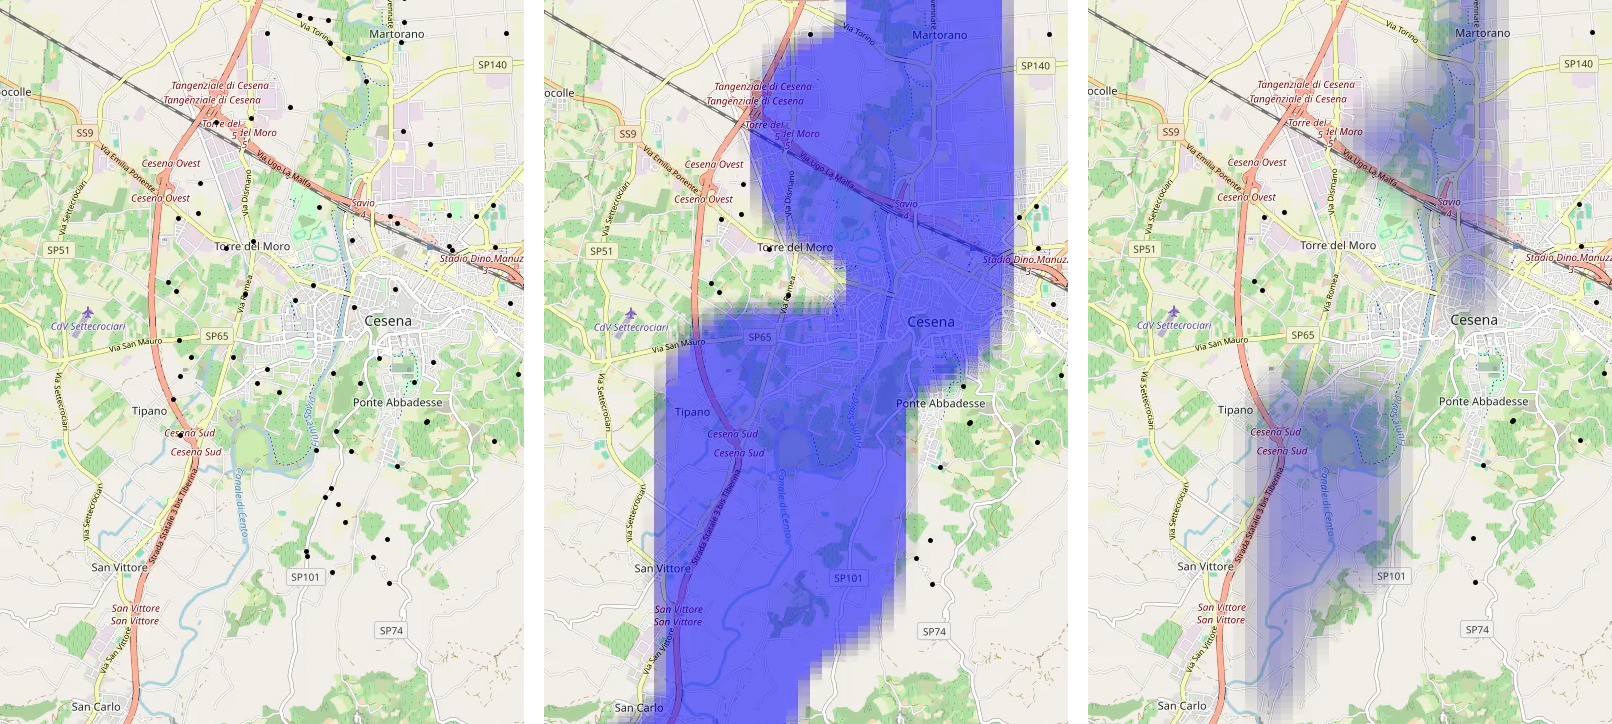
\includegraphics[width=\linewidth]{figures/validazione/alluvione.png}
  \caption[La simulazione dimostrativa in istanti successivi]{La simulazione in
  tre istanti successivi. Da sinistra: prima degli eventi,
  durante l'esondazione del fiume Savio, la riduzione della portata.}
  \label{fig:caso-studio}
\end{figure}

Nelle immagini, in ordine da sinistra verso destra:

\begin{enumerate}
  \item 25 aprile 2023, 00:00 UTC (tempo di simulazione 0): la portata fluviale
  del fiume Savio rientra nella norma;
  \item 16 maggio 2023, 15:00 UTC (tempo di simulazione 519): il fiume Savio straripa.
  I nodi che rilevano nella propria posizione un valore oltre la soglia di allerta
  si spostano fuori dalla zona;
  \item 21 maggio 2023, 04:00 UTC (tempo di simulazione 580): la portata fluviale
  si riduce. I nodi che sono stati allertati rimangono fuori dalla zona.
\end{enumerate}

Riavviando la simulazione con la stessa configurazione, il gestore della cache
trova la voce e il layer viene costruito senza alcuna richiesta di rete
(\Cref{lst:log-cache-hit}), a verifica di \req{F9} e \req{F10}.

\lstinputlisting[
    language={},
    keywordstyle={},
    stringstyle={},
    commentstyle={},
    label={lst:log-cache-hit},
    caption={[Log della seconda esecuzione.]{Messaggio del modulo alla seconda esecuzione con la stessa configurazione. Prefisso del logger omesso.}}
]{listings/validazione/cache_hit.txt}

La chiave della voce è derivata dall'endpoint, dal dataset e dal contenuto della
richiesta. I parametri che non ne fanno parte, come l'origine temporale o la
strategia di interpolazione, possono quindi cambiare fra un'esecuzione e l'altra
senza provocare un nuovo scaricamento.

L'esecuzione è stata ripetuta con successo anche eliminando il file \texttt{.cdsapirc},
il quale contiene la chiave ECMWF, a conferma che esso viene letto solo quando
una richiesta di rete si rende necessaria.

%----------------------------------------------------------------------------------------
% CAPITOLO 7 (CONCLUSIONI)
%----------------------------------------------------------------------------------------

\chapter{Conclusioni}
\label{chap:conclusioni}

\section{Il lavoro svolto}
\label{sec:riepilogo}

L'obiettivo del lavoro era riuscire a dotare Alchemist della capacità
di esporre ai nodi di una simulazione grandezze geospaziali misurate,
in funzione della posizione in cui essi si trovano e dell'istante di
simulazione in cui le richiedono, ottenendole dai data store Copernicus.
Il risultato ottenuto è un nuovo modulo del simulatore, organizzato
nei quattro sottomoduli descritti nel \Cref{chap:progettazione} e
dichiarabile interamente nella configurazione della simulazione.

Il sotto-obiettivo di rappresentazione è stato soddisfatto da \texttt{RasterGrid}
e \texttt{GridSnapshots}, che descrivono rispettivamente una griglia di campioni
e una successione di griglie omogenee, indipendenti dal formato e dalla fonte
da cui tali dati provengono. Queste astrazioni portano con sé l'estensione
spaziale e temporale nelle quali la grandezza di riferimento è nota, e trattano
in modo esplicito le celle prive di misura (\req{F7}); delle griglie sono fornite
una realizzazione densa e una sparsa, scelte dinamicamente durante la costruzione
della serie in funzione della densità delle singole griglie.

Il sotto-obiettivo di risoluzione è stato soddisfatto dal layer e dalle strategie
a cui esso delega. Il layer stabilisce alla costruzione la corrispondenza fra
il tempo di simulazione e gli istanti del mondo reale, dichiarata da chi
configura la simulazione anziché fissata dal modulo (\req{F3}),
trova i campioni pertinenti all'istante in cui viene interrogato e incarica
la produzione del valore a una strategia di interpolazione e a un convertitore,
entrambi intercambiabili e dichiarabili dalla configurazione (\req{F5}, \req{F6}, \req{F11}).

Il sotto-obiettivo di acquisizione è stato soddisfatto dal sottosistema
costituito da \texttt{CacheKey}, \texttt{ExternalDataProvider} e \texttt{CacheManager},
e dalle loro realizzazioni che dialogano con i tre data store Copernicus.
L'identità stessa di una richiesta ne decide deterministicamente la voce
di cache (\req{NF4}), cosa che rende possibile riusare dati già acquisiti
senza alcuna richiesta di rete (\req{F10}); tutta l'acquisizione avviene
al caricamento della simulazione, in modo tale che ogni condizione che
impedisca di disporre dei dati si manifesti prima che l'esecuzione cominci (\req{NF6}).
Un risultato aggiuntivo riguarda il protocollo dei data store Copernicus:
il loro comportamento aderisce solo in parte a \ac{OGC} API
Processes, e gli scostamenti riscontrati, discussi nel \Cref{chap:implementazione},
non sono documentati dal servizio: sono stati verificati empiricamente, a partire
dalle risposte reali raccolte dallo sviluppo, e la loro descrizione
resta valida anche per altri scenari d'utilizzo.

Il lavoro descritto ha potuto realizzarsi come aggiunta
al simulatore, senza modifiche alle
astrazioni del suo modello (\req{NF1}).

La validazione copre tutte e tre le parti: una suite di test
che non dipende dai data store né dal possesso di credenziali (\req{NF3}),
la verifica del caricamento da configurazione, l'uso del client sui data
store reali, una simulazione dimostrativa per confermare il corretto comportamento
del sistema di cache e la corretta lettura ed esposizione dei valori.

\section{I limiti della soluzione}
\label{sec:limiti}

Il modulo opera entro alcune ipotesi e alcune scelte prese.

\begin{itemize}
  \item \textbf{La forma della griglia}: l'ipotesi stabilita nella
  \Cref{subsec:griglie-supportate} esclude dataset campionati su griglia
  nativa in proiezione cartografica. Tali dati restano utilizzabili solo se
  ricondotti esternamente a una griglia di assi indipendenti e caricati poi
  tramite il secondo costruttore del layer.

  \item \textbf{Le dimensioni del dato}: la grandezza esposta deve
  dipendere dalle sole tre dimensioni tempo, latitudine e longitudine. I dataset
  che sono definiti anche su altre dimensioni, come quota o livello di pressione,
  non possono individuare un valore unico per una posizione e un istante, e restano
  quindi fuori dal campo di applicabilità.

  \item \textbf{L'occupazione di memoria}: la realizzazione fornita della serie
  di griglie costruisce l'intera successione in memoria al caricamento,
  scelta che risponde a \req{NF7} ma il cui costo cresce con l'estensione temporale
  e geografica della richiesta.

  \item \textbf{La sola lettura}: il valore esposto cambia soltanto perché il
  tempo di simulazione avanza lungo una serie di griglie già disponibile. Il dato
  sottostante non può quindi essere aggiornato durante l'esecuzione.
  Resta quindi fuori portata ogni
  scenario in cui l'ambiente conserva l'effetto di ciò che i nodi hanno fatto,
  ad esempio una simulazione in cui dei depuratori riducono la concentrazione
  degli inquinanti nella zona in cui operano.

  \item \textbf{La conoscenza preventiva del nome della variabile}: quando i file
  contengono più di una grandezza, la configurazione deve indicare quale far esporre
  al layer, e il nome da indicare è quello interno al file, che non coincide
  con quello utilizzato per fare la richiesta verso il data store.
  Nella modalità che acquisisce i dati da un data store tale nome è noto prima
  che l'acquisizione sia avvenuta: chi conduce la simulazione deve eseguirla una
  prima volta, o ispezionare i file ottenuti, per apprenderlo. Il caso è più marcato
  con i file GRIB, nei quali la grandezza è identificata da codici numerici e il
  nome esposto dipende dalle tabelle che la libreria di lettura possiede
  (\Cref{sec:formati-raster}).
\end{itemize}

\section{Sviluppi futuri}
\label{sec:sviluppi-futuri}

La struttura del modulo rende possibile alcune direzioni di sviluppo future senza
modificarne le parti già esistenti.

La prima è il superamento della restrizione sulla forma della griglia.
Rappresentare dataset in proiezione cartografica richiede di invertire la proiezione
fra il sistema di riferimento del dataset e quello geografico, in modo da poter
individuare la cella contenente una determinata posizione; ciò si traduce
in una nuova realizzazione di \texttt{RasterGrid}, che il resto del modulo
può usare tramite la stessa astrazione.

La seconda riguarda le fonti di dati. Il sottosistema di acquisizione
conosce i data store Copernicus solo nelle realizzazioni che ne descrivono
una richiesta e li interrogano: utilizzare una fonte diversa richiede unicamente
di implementare la coppia \texttt{CacheKey} ed \texttt{ExternalDataProvider}
corrispondente. Il caso più immediato è il recupero autonomo da parte del simulatore
degli estratti cartografici utili ad alimentare un \texttt{OSMEnvironment}, che oggi
devono essere predisposti manualmente.

Una terza direzione è una realizzazione della serie di griglie che carichi
i dati su richiesta invece che per intero all'avvio della simulazione,
con un compromesso tra occupazione di memoria e costo di lettura.
Il layer non richiederebbe alcuna modifica poiché basterebbe dare una nuova
implementazione di \texttt{GridSnapshots}.

Le ultime due dipendono invece da interventi sul simulatore.
Una revisione del motore di simulazione renderebbe possibile l'impiego
di layer aggiornabili durante l'esecuzione. Una migrazione del tipo di tempo
di Alchemist (della quale la \Cref{subsec:corrispondenza-temporale} riporta lo studio di fattibilità),
o un sistema di conversione generica dal tempo di simulazione
a una rappresentazione arbitraria del tempo, semplificherebbe la corrispondenza
fra i due domini temporali incontrati nel lavoro svolto; poiché tale 
corrispondenza è stabilita unicamente nel layer, l'impatto di eventuali
modifiche sul dominio temporale resterebbero circoscritte a esso.


%----------------------------------------------------------------------------------------
% BIBLIOGRAPHY
%----------------------------------------------------------------------------------------

\backmatter

\bibliographystyle{alpha}
\bibliography{bibliography}

%\begin{acknowledgements} % this is optional
%Optional. Max 1 page.
%\end{acknowledgements}

\end{document}
